

% Plantilla para un Trabajo Fin de Grado de la Universidad de Granada,
% adaptada para el Doble Grado en Ingeniería Informática y Matemáticas.
%
%  Autor de la plantilla original: Mario Román.
%  Enlace: https://github.com/mroman42/templates
%  Cambios en la plantilla por: Luis Ortega
%  Licencia: GNU GPLv2.
%
%
% Esta plantilla es una adaptación al castellano de la plantilla
% classicthesis de André Miede, que puede obtenerse en:
%  https://ctan.org/tex-archive/macros/latex/contrib/classicthesis?lang=en
% La plantilla original se licencia en GNU GPLv2.
%
% Esta plantilla usa símbolos de la Universidad de Granada sujetos a la normativa
% de identidad visual corporativa, que puede encontrarse en:
% http://secretariageneral.ugr.es/pages/ivc/normativa
%
% La compilación se realiza con las siguientes instrucciones:
%   pdflatex --shell-escape main.tex
%   bibtex main
%   pdflatex --shell-escape main.tex
%   pdflatex --shell-escape main.tex

% Opciones del tipo de documento
\documentclass[twoside,openright,titlepage,numbers=noenddot,openany,headinclude,footinclude=true, cleardoublepage=empty,abstractoff,BCOR=5mm,paper=a4,fontsize=11pt]{scrreprt}

% Paquetes de latex que se cargan al inicio. Cubren la entrada de
% texto, gráficos, código fuente y símbolos.
\usepackage{relsize}
\usepackage[utf8]{inputenc}
\usepackage[T1]{fontenc}
\usepackage{fixltx2e}
\usepackage{graphicx} % Inclusión de imágenes.
\usepackage{grffile}  % Distintos formatos para imágenes.
\usepackage{longtable} % Tablas multipágina.
\usepackage{wrapfig} % Coloca texto alrededor de una figura.
\usepackage{rotating}
\usepackage[normalem]{ulem}
\usepackage{amsmath}
\usepackage{textcomp}
\usepackage{amssymb}
\usepackage{capt-of}
\usepackage[colorlinks=true]{hyperref}
\usepackage{tikz} % Diagramas conmutativos.
\usepackage{pgfplots}
\usepackage{dcolumn}
\usepackage{booktabs}
\usepackage{minted} % Código fuente.
\usepackage{natbib}
\usepackage{bm}
\usepackage{centernot}
\usetikzlibrary{positioning}
\usetikzlibrary{bayesnet}
\usetikzlibrary{shapes.geometric}


\usepackage{caption}

% Plantilla classicthesis
\usepackage[beramono,eulerchapternumbers,linedheaders,parts,a5paper,dottedtoc,
manychapters,pdfspacing]{classicthesis}

% Geometría y espaciado de párrafos.
\setcounter{secnumdepth}{0}
\usepackage{enumitem}
\setitemize{noitemsep,topsep=0pt,parsep=0pt,partopsep=0pt}
\setlist[enumerate]{topsep=0pt,itemsep=-1ex,partopsep=1ex,parsep=1ex}
\usepackage[top=1in, bottom=1.5in, left=0.9in, right=1.2in]{geometry}
\setlength\itemsep{0em}
\setlength{\parindent}{0pt}
\usepackage{parskip}

% Algoritmos
\usepackage[ruled,vlined]{algorithm2e}

% Todo notes
\usepackage{todonotes}
\let\marginpar\oldmarginpar



% Profundidad de la tabla de contenidos.
\setcounter{secnumdepth}{3}

% Usa el paquete minted para mostrar trozos de código.
% Pueden seleccionarse el lenguaje apropiado y el estilo del código.
\usepackage{minted}
\usemintedstyle{colorful}
\setminted{fontsize=\small}
\renewcommand{\theFancyVerbLine}{\sffamily\textcolor[rgb]{0.5,0.5,1.0}{\oldstylenums{\arabic{FancyVerbLine}}}}

% Archivos de configuración.
%------------------------
% Bibliotecas para matemáticas de latex
%------------------------
\usepackage{amsthm}
\usepackage{amsmath}
\usepackage{tikz}
\usepackage{tikz-cd}
\usetikzlibrary{shapes,fit}
\usepackage{bussproofs}
\EnableBpAbbreviations{}
\usepackage{mathtools}
\usepackage{scalerel}
\usepackage{stmaryrd}

%------------------------
% Estilos para los teoremas
%------------------------
\theoremstyle{plain}
\newtheorem{theorem}{Theorem}
\newtheorem{proposition}{Proposition}
\newtheorem{lemma}{Lemma}
\newtheorem{corollary}{Corollary}
\theoremstyle{definition}
\newtheorem{definition}{Definition}
\newtheorem{proofs}{Proof}
\theoremstyle{remark}
\newtheorem{remark}{Remark}
\newtheorem{exampleth}{Example}

\begingroup\makeatletter\@for\theoremstyle:=definition,remark,plain\do{\expandafter\g@addto@macro\csname th@\theoremstyle\endcsname{\addtolength\thm@preskip\parskip}}\endgroup

%------------------------
% Macros
% ------------------------

% Aquí pueden añadirse abreviaturas para comandos de latex
% frequentemente usados.
\newcommand*\diff{\mathop{}\!\mathrm{d}}
\newcommand{\R}{\mathbb{R}}
% \newcommand{\E}{\mathbb{E}}
\newcommand{\bmu}{\bm{\mu}}
\newcommand{\bx}{\bm{x}}
\newcommand{\bX}{\bm{X}}
\newcommand{\bz}{\bm{z}}
\newcommand{\bZ}{\bm{Z}}
\newcommand{\bv}{\bm{v}}
\newcommand{\bh}{\bm{h}}
\newcommand{\bSigma}{\bm{\Sigma}}
\newcommand{\bpi}{\bm{\pi}}
\newcommand{\bLambda}{\bm{\Lambda}}
\newcommand{\btheta}{\bm{\theta}}

\newcommand{\V}{\mathcal{V}}
\newcommand{\D}{\mathcal{D}}
\newcommand{\X}{\mathcal{X}}
\newcommand{\I}{\mathcal{I}}

\newcommand\ddfrac[2]{\frac{\displaystyle #1}{\displaystyle #2}}

\newcommand\E[2]{\mathbb{E}_{#1}\Big[#2\Big]}
\newcommand\KL[2]{KL\Big(#1 \bigm| #2\Big)}
\newcommand{\bigCI}{\mathrel{\text{\scalebox{1.07}{$\perp\mkern-10mu\perp$}}}}
\newcommand{\bigCD}{\centernot{\bigCI}}

\DeclareMathOperator*{\argmax}{arg\,max}
\DeclareMathOperator*{\argmin}{arg\,min}
  % En macros.tex se almacenan las opciones y comandos para escribir matemáticas.
% ****************************************************************************************************
% classicthesis-config.tex 
% formerly known as loadpackages.sty, classicthesis-ldpkg.sty, and classicthesis-preamble.sty 
% Use it at the beginning of your ClassicThesis.tex, or as a LaTeX Preamble 
% in your ClassicThesis.{tex,lyx} with % ****************************************************************************************************
% classicthesis-config.tex 
% formerly known as loadpackages.sty, classicthesis-ldpkg.sty, and classicthesis-preamble.sty 
% Use it at the beginning of your ClassicThesis.tex, or as a LaTeX Preamble 
% in your ClassicThesis.{tex,lyx} with % ****************************************************************************************************
% classicthesis-config.tex 
% formerly known as loadpackages.sty, classicthesis-ldpkg.sty, and classicthesis-preamble.sty 
% Use it at the beginning of your ClassicThesis.tex, or as a LaTeX Preamble 
% in your ClassicThesis.{tex,lyx} with \input{classicthesis-config}
% ****************************************************************************************************  
% If you like the classicthesis, then I would appreciate a postcard. 
% My address can be found in the file ClassicThesis.pdf. A collection 
% of the postcards I received so far is available online at 
% http://postcards.miede.de
% ****************************************************************************************************


% ****************************************************************************************************
% 0. Set the encoding of your files. UTF-8 is the only sensible encoding nowadays. If you can't read
% äöüßáéçèê∂åëæƒÏ€ then change the encoding setting in your editor, not the line below. If your editor
% does not support utf8 use another editor!
% ****************************************************************************************************
\PassOptionsToPackage{utf8x}{inputenc}
	\usepackage{inputenc}

% ****************************************************************************************************
% 1. Configure classicthesis for your needs here, e.g., remove "drafting" below 
% in order to deactivate the time-stamp on the pages
% ****************************************************************************************************
\PassOptionsToPackage{eulerchapternumbers,listings,drafting,%
		pdfspacing,%floatperchapter,%linedheaders,%
                subfig,beramono,eulermath,parts,dottedtoc}{classicthesis}                                        
% ********************************************************************
% Available options for classicthesis.sty 
% (see ClassicThesis.pdf for more information):
% drafting
% parts nochapters linedheaders
% eulerchapternumbers beramono eulermath pdfspacing minionprospacing
% tocaligned dottedtoc manychapters
% listings floatperchapter subfig
% ********************************************************************

% ****************************************************************************************************
% 2. Personal data and user ad-hoc commands
% ****************************************************************************************************
\newcommand{\myTitle}{A Classic Thesis Style\xspace}
\newcommand{\mySubtitle}{An Homage to The Elements of Typographic Style\xspace}
\newcommand{\myDegree}{Doktor-Ingenieur (Dr.-Ing.)\xspace}
\newcommand{\myName}{André Miede\xspace}
\newcommand{\myProf}{Put name here\xspace}
\newcommand{\myOtherProf}{Put name here\xspace}
\newcommand{\mySupervisor}{Put name here\xspace}
\newcommand{\myFaculty}{Put data here\xspace}
\newcommand{\myDepartment}{Put data here\xspace}
\newcommand{\myUni}{Put data here\xspace}
\newcommand{\myLocation}{Saarbrücken\xspace}
\newcommand{\myTime}{September 2015\xspace}
%\newcommand{\myVersion}{version 4.2\xspace}

% ********************************************************************
% Setup, finetuning, and useful commands
% ********************************************************************
\newcounter{dummy} % necessary for correct hyperlinks (to index, bib, etc.)
\newlength{\abcd} % for ab..z string length calculation
\providecommand{\mLyX}{L\kern-.1667em\lower.25em\hbox{Y}\kern-.125emX\@}
\newcommand{\ie}{i.\,e.}
\newcommand{\Ie}{I.\,e.}
\newcommand{\eg}{e.\,g.}
\newcommand{\Eg}{E.\,g.} 
% ****************************************************************************************************


% ****************************************************************************************************
% 3. Loading some handy packages
% ****************************************************************************************************
% ******************************************************************** 
% Packages with options that might require adjustments
% ******************************************************************** 
%\PassOptionsToPackage{ngerman,american}{babel}   % change this to your language(s)
% Spanish languages need extra options in order to work with this template
% \PassOptionsToPackage{es-lcroman,spanish}{babel}
\usepackage[main=english]{babel}

%\usepackage{csquotes}
% \PassOptionsToPackage{%
%     %backend=biber, %instead of bibtex
% 	backend=bibtex8,bibencoding=ascii,%
% 	language=auto,%
% 	style=alpha,%
%     %style=authoryear-comp, % Author 1999, 2010
%     %bibstyle=authoryear,dashed=false, % dashed: substitute rep. author with ---
%     sorting=nyt, % name, year, title
%     maxbibnames=10, % default: 3, et al.
%     %backref=true,%
%     natbib=true % natbib compatibility mode (\citep and \citet still work)
% }{biblatex}
%     \usepackage{biblatex}

% \PassOptionsToPackage{fleqn}{amsmath}       % math environments and more by the AMS 
%     \usepackage{amsmath}

% ******************************************************************** 
% General useful packages
% ******************************************************************** 
\PassOptionsToPackage{T1}{fontenc} % T2A for cyrillics
    \usepackage{fontenc}     
\usepackage{textcomp} % fix warning with missing font shapes
\usepackage{scrhack} % fix warnings when using KOMA with listings package          
\usepackage{xspace} % to get the spacing after macros right  
\usepackage{mparhack} % get marginpar right
\usepackage{fixltx2e} % fixes some LaTeX stuff --> since 2015 in the LaTeX kernel (see below)
%\usepackage[latest]{latexrelease} % will be used once available in more distributions (ISSUE #107)
\PassOptionsToPackage{printonlyused,smaller}{acronym} 
    \usepackage{acronym} % nice macros for handling all acronyms in the thesis
    %\renewcommand{\bflabel}[1]{{#1}\hfill} % fix the list of acronyms --> no longer working
    %\renewcommand*{\acsfont}[1]{\textsc{#1}} 
    \renewcommand*{\aclabelfont}[1]{\acsfont{#1}}
% ****************************************************************************************************


% ****************************************************************************************************
% 4. Setup floats: tables, (sub)figures, and captions
% ****************************************************************************************************
\usepackage{tabularx} % better tables
    \setlength{\extrarowheight}{3pt} % increase table row height
\newcommand{\tableheadline}[1]{\multicolumn{1}{c}{\spacedlowsmallcaps{#1}}}
\newcommand{\myfloatalign}{\centering} % to be used with each float for alignment
\usepackage{caption}
% Thanks to cgnieder and Claus Lahiri
% http://tex.stackexchange.com/questions/69349/spacedlowsmallcaps-in-caption-label
% [REMOVED DUE TO OTHER PROBLEMS, SEE ISSUE #82]    
%\DeclareCaptionLabelFormat{smallcaps}{\bothIfFirst{#1}{~}\MakeTextLowercase{\textsc{#2}}}
%\captionsetup{font=small,labelformat=smallcaps} % format=hang,
\captionsetup{font=small} % format=hang,
\usepackage{subfig}  
% ****************************************************************************************************


% ****************************************************************************************************
% 5. Setup code listings
% ****************************************************************************************************
% \usepackage{listings} 
% %\lstset{emph={trueIndex,root},emphstyle=\color{BlueViolet}}%\underbar} % for special keywords
% \lstset{language={Haskell},morekeywords={PassOptionsToPackage,selectlanguage},keywordstyle=\color{RoyalBlue},basicstyle=\small\ttfamily,commentstyle=\color{Green}\ttfamily,stringstyle=\rmfamily,numbers=none,numberstyle=\scriptsize,stepnumber=5,numbersep=8pt,showstringspaces=false,breaklines=true,belowcaptionskip=.75\baselineskip} 
% ****************************************************************************************************             


% ****************************************************************************************************
% 6. PDFLaTeX, hyperreferences and citation backreferences
% ****************************************************************************************************
% ********************************************************************
% Using PDFLaTeX
% ********************************************************************
\PassOptionsToPackage{pdftex,hyperfootnotes=false,pdfpagelabels}{hyperref}
    \usepackage{hyperref}  % backref linktocpage pagebackref
\pdfcompresslevel=9
\pdfadjustspacing=1 
\PassOptionsToPackage{pdftex}{graphicx}
    \usepackage{graphicx} 
 

% ********************************************************************
% Hyperreferences
% ********************************************************************
\hypersetup{%
    %draft, % = no hyperlinking at all (useful in b/w printouts)
    colorlinks=true, linktocpage=true, pdfstartpage=3, pdfstartview=FitV,%
    % uncomment the following line if you want to have black links (e.g., for printing)
    %colorlinks=false, linktocpage=false, pdfstartpage=3, pdfstartview=FitV, pdfborder={0 0 0},%
    breaklinks=true, pdfpagemode=UseNone, pageanchor=true, pdfpagemode=UseOutlines,%
    plainpages=false, bookmarksnumbered, bookmarksopen=true, bookmarksopenlevel=1,%
    hypertexnames=true, pdfhighlight=/O,%nesting=true,%frenchlinks,%
    urlcolor=webbrown, linkcolor=RoyalBlue, citecolor=webgreen, %pagecolor=RoyalBlue,%
    %urlcolor=Black, linkcolor=Black, citecolor=Black, %pagecolor=Black,%
    pdftitle={\myTitle},%
    pdfauthor={\textcopyright\ \myName, \myUni, \myFaculty},%
    pdfsubject={},%
    pdfkeywords={},%
    pdfcreator={pdfLaTeX},%
    pdfproducer={LaTeX with hyperref and classicthesis}%
}   

% ********************************************************************
% Setup autoreferences
% ********************************************************************
% There are some issues regarding autorefnames
% http://www.ureader.de/msg/136221647.aspx
% http://www.tex.ac.uk/cgi-bin/texfaq2html?label=latexwords
% you have to redefine the makros for the 
% language you use, e.g., american, ngerman
% (as chosen when loading babel/AtBeginDocument)
% ********************************************************************
\makeatletter
\@ifpackageloaded{babel}%
    {%
       \addto\extrasamerican{%
			\renewcommand*{\figureautorefname}{Figure}%
			\renewcommand*{\tableautorefname}{Table}%
			\renewcommand*{\partautorefname}{Part}%
			\renewcommand*{\chapterautorefname}{Chapter}%
			\renewcommand*{\sectionautorefname}{Section}%
			\renewcommand*{\subsectionautorefname}{Section}%
			\renewcommand*{\subsubsectionautorefname}{Section}%     
                }%
       \addto\extrasngerman{% 
			\renewcommand*{\paragraphautorefname}{Absatz}%
			\renewcommand*{\subparagraphautorefname}{Unterabsatz}%
			\renewcommand*{\footnoteautorefname}{Fu\"snote}%
			\renewcommand*{\FancyVerbLineautorefname}{Zeile}%
			\renewcommand*{\theoremautorefname}{Theorem}%
			\renewcommand*{\appendixautorefname}{Anhang}%
			\renewcommand*{\equationautorefname}{Gleichung}%        
			\renewcommand*{\itemautorefname}{Punkt}%
                }%  
            % Fix to getting autorefs for subfigures right (thanks to Belinda Vogt for changing the definition)
            \providecommand{\subfigureautorefname}{\figureautorefname}%             
    }{\relax}
\makeatother


% ****************************************************************************************************
% 7. Last calls before the bar closes
% ****************************************************************************************************
% ********************************************************************
% Development Stuff
% ********************************************************************
\listfiles
%\PassOptionsToPackage{l2tabu,orthodox,abort}{nag}
%   \usepackage{nag}
%\PassOptionsToPackage{warning, all}{onlyamsmath}
%   \usepackage{onlyamsmath}

% ********************************************************************
% Last, but not least...
% ********************************************************************
\usepackage{classicthesis} 
% ****************************************************************************************************


% ****************************************************************************************************
% 8. Further adjustments (experimental)
% ****************************************************************************************************
% ********************************************************************
% Changing the text area
% ********************************************************************
\linespread{1.05} % a bit more for Palatino
% \areaset[current]{325pt}{680pt} % 686 (factor 2.2) + 33 head + 42 head \the\footskip
%\setlength{\marginparwidth}{7em}%
%\setlength{\marginparsep}{2em}%

% ********************************************************************
% Using different fonts
% ********************************************************************
%\usepackage[oldstylenums]{kpfonts} % oldstyle notextcomp
%\usepackage[osf]{libertine}
%\usepackage[light,condensed,math]{iwona}
%\renewcommand{\sfdefault}{iwona}
%\usepackage{lmodern} % <-- no osf support :-(
%\usepackage{cfr-lm} % 
%\usepackage[urw-garamond]{mathdesign} <-- no osf support :-(
%\usepackage[default,osfigures]{opensans} % scale=0.95 
%\usepackage[sfdefault]{FiraSans}
% ****************************************************************************************************

% ****************************************************************************************************  
% If you like the classicthesis, then I would appreciate a postcard. 
% My address can be found in the file ClassicThesis.pdf. A collection 
% of the postcards I received so far is available online at 
% http://postcards.miede.de
% ****************************************************************************************************


% ****************************************************************************************************
% 0. Set the encoding of your files. UTF-8 is the only sensible encoding nowadays. If you can't read
% äöüßáéçèê∂åëæƒÏ€ then change the encoding setting in your editor, not the line below. If your editor
% does not support utf8 use another editor!
% ****************************************************************************************************
\PassOptionsToPackage{utf8x}{inputenc}
	\usepackage{inputenc}

% ****************************************************************************************************
% 1. Configure classicthesis for your needs here, e.g., remove "drafting" below 
% in order to deactivate the time-stamp on the pages
% ****************************************************************************************************
\PassOptionsToPackage{eulerchapternumbers,listings,drafting,%
		pdfspacing,%floatperchapter,%linedheaders,%
                subfig,beramono,eulermath,parts,dottedtoc}{classicthesis}                                        
% ********************************************************************
% Available options for classicthesis.sty 
% (see ClassicThesis.pdf for more information):
% drafting
% parts nochapters linedheaders
% eulerchapternumbers beramono eulermath pdfspacing minionprospacing
% tocaligned dottedtoc manychapters
% listings floatperchapter subfig
% ********************************************************************

% ****************************************************************************************************
% 2. Personal data and user ad-hoc commands
% ****************************************************************************************************
\newcommand{\myTitle}{A Classic Thesis Style\xspace}
\newcommand{\mySubtitle}{An Homage to The Elements of Typographic Style\xspace}
\newcommand{\myDegree}{Doktor-Ingenieur (Dr.-Ing.)\xspace}
\newcommand{\myName}{André Miede\xspace}
\newcommand{\myProf}{Put name here\xspace}
\newcommand{\myOtherProf}{Put name here\xspace}
\newcommand{\mySupervisor}{Put name here\xspace}
\newcommand{\myFaculty}{Put data here\xspace}
\newcommand{\myDepartment}{Put data here\xspace}
\newcommand{\myUni}{Put data here\xspace}
\newcommand{\myLocation}{Saarbrücken\xspace}
\newcommand{\myTime}{September 2015\xspace}
%\newcommand{\myVersion}{version 4.2\xspace}

% ********************************************************************
% Setup, finetuning, and useful commands
% ********************************************************************
\newcounter{dummy} % necessary for correct hyperlinks (to index, bib, etc.)
\newlength{\abcd} % for ab..z string length calculation
\providecommand{\mLyX}{L\kern-.1667em\lower.25em\hbox{Y}\kern-.125emX\@}
\newcommand{\ie}{i.\,e.}
\newcommand{\Ie}{I.\,e.}
\newcommand{\eg}{e.\,g.}
\newcommand{\Eg}{E.\,g.} 
% ****************************************************************************************************


% ****************************************************************************************************
% 3. Loading some handy packages
% ****************************************************************************************************
% ******************************************************************** 
% Packages with options that might require adjustments
% ******************************************************************** 
%\PassOptionsToPackage{ngerman,american}{babel}   % change this to your language(s)
% Spanish languages need extra options in order to work with this template
% \PassOptionsToPackage{es-lcroman,spanish}{babel}
\usepackage[main=english]{babel}

%\usepackage{csquotes}
% \PassOptionsToPackage{%
%     %backend=biber, %instead of bibtex
% 	backend=bibtex8,bibencoding=ascii,%
% 	language=auto,%
% 	style=alpha,%
%     %style=authoryear-comp, % Author 1999, 2010
%     %bibstyle=authoryear,dashed=false, % dashed: substitute rep. author with ---
%     sorting=nyt, % name, year, title
%     maxbibnames=10, % default: 3, et al.
%     %backref=true,%
%     natbib=true % natbib compatibility mode (\citep and \citet still work)
% }{biblatex}
%     \usepackage{biblatex}

% \PassOptionsToPackage{fleqn}{amsmath}       % math environments and more by the AMS 
%     \usepackage{amsmath}

% ******************************************************************** 
% General useful packages
% ******************************************************************** 
\PassOptionsToPackage{T1}{fontenc} % T2A for cyrillics
    \usepackage{fontenc}     
\usepackage{textcomp} % fix warning with missing font shapes
\usepackage{scrhack} % fix warnings when using KOMA with listings package          
\usepackage{xspace} % to get the spacing after macros right  
\usepackage{mparhack} % get marginpar right
\usepackage{fixltx2e} % fixes some LaTeX stuff --> since 2015 in the LaTeX kernel (see below)
%\usepackage[latest]{latexrelease} % will be used once available in more distributions (ISSUE #107)
\PassOptionsToPackage{printonlyused,smaller}{acronym} 
    \usepackage{acronym} % nice macros for handling all acronyms in the thesis
    %\renewcommand{\bflabel}[1]{{#1}\hfill} % fix the list of acronyms --> no longer working
    %\renewcommand*{\acsfont}[1]{\textsc{#1}} 
    \renewcommand*{\aclabelfont}[1]{\acsfont{#1}}
% ****************************************************************************************************


% ****************************************************************************************************
% 4. Setup floats: tables, (sub)figures, and captions
% ****************************************************************************************************
\usepackage{tabularx} % better tables
    \setlength{\extrarowheight}{3pt} % increase table row height
\newcommand{\tableheadline}[1]{\multicolumn{1}{c}{\spacedlowsmallcaps{#1}}}
\newcommand{\myfloatalign}{\centering} % to be used with each float for alignment
\usepackage{caption}
% Thanks to cgnieder and Claus Lahiri
% http://tex.stackexchange.com/questions/69349/spacedlowsmallcaps-in-caption-label
% [REMOVED DUE TO OTHER PROBLEMS, SEE ISSUE #82]    
%\DeclareCaptionLabelFormat{smallcaps}{\bothIfFirst{#1}{~}\MakeTextLowercase{\textsc{#2}}}
%\captionsetup{font=small,labelformat=smallcaps} % format=hang,
\captionsetup{font=small} % format=hang,
\usepackage{subfig}  
% ****************************************************************************************************


% ****************************************************************************************************
% 5. Setup code listings
% ****************************************************************************************************
% \usepackage{listings} 
% %\lstset{emph={trueIndex,root},emphstyle=\color{BlueViolet}}%\underbar} % for special keywords
% \lstset{language={Haskell},morekeywords={PassOptionsToPackage,selectlanguage},keywordstyle=\color{RoyalBlue},basicstyle=\small\ttfamily,commentstyle=\color{Green}\ttfamily,stringstyle=\rmfamily,numbers=none,numberstyle=\scriptsize,stepnumber=5,numbersep=8pt,showstringspaces=false,breaklines=true,belowcaptionskip=.75\baselineskip} 
% ****************************************************************************************************             


% ****************************************************************************************************
% 6. PDFLaTeX, hyperreferences and citation backreferences
% ****************************************************************************************************
% ********************************************************************
% Using PDFLaTeX
% ********************************************************************
\PassOptionsToPackage{pdftex,hyperfootnotes=false,pdfpagelabels}{hyperref}
    \usepackage{hyperref}  % backref linktocpage pagebackref
\pdfcompresslevel=9
\pdfadjustspacing=1 
\PassOptionsToPackage{pdftex}{graphicx}
    \usepackage{graphicx} 
 

% ********************************************************************
% Hyperreferences
% ********************************************************************
\hypersetup{%
    %draft, % = no hyperlinking at all (useful in b/w printouts)
    colorlinks=true, linktocpage=true, pdfstartpage=3, pdfstartview=FitV,%
    % uncomment the following line if you want to have black links (e.g., for printing)
    %colorlinks=false, linktocpage=false, pdfstartpage=3, pdfstartview=FitV, pdfborder={0 0 0},%
    breaklinks=true, pdfpagemode=UseNone, pageanchor=true, pdfpagemode=UseOutlines,%
    plainpages=false, bookmarksnumbered, bookmarksopen=true, bookmarksopenlevel=1,%
    hypertexnames=true, pdfhighlight=/O,%nesting=true,%frenchlinks,%
    urlcolor=webbrown, linkcolor=RoyalBlue, citecolor=webgreen, %pagecolor=RoyalBlue,%
    %urlcolor=Black, linkcolor=Black, citecolor=Black, %pagecolor=Black,%
    pdftitle={\myTitle},%
    pdfauthor={\textcopyright\ \myName, \myUni, \myFaculty},%
    pdfsubject={},%
    pdfkeywords={},%
    pdfcreator={pdfLaTeX},%
    pdfproducer={LaTeX with hyperref and classicthesis}%
}   

% ********************************************************************
% Setup autoreferences
% ********************************************************************
% There are some issues regarding autorefnames
% http://www.ureader.de/msg/136221647.aspx
% http://www.tex.ac.uk/cgi-bin/texfaq2html?label=latexwords
% you have to redefine the makros for the 
% language you use, e.g., american, ngerman
% (as chosen when loading babel/AtBeginDocument)
% ********************************************************************
\makeatletter
\@ifpackageloaded{babel}%
    {%
       \addto\extrasamerican{%
			\renewcommand*{\figureautorefname}{Figure}%
			\renewcommand*{\tableautorefname}{Table}%
			\renewcommand*{\partautorefname}{Part}%
			\renewcommand*{\chapterautorefname}{Chapter}%
			\renewcommand*{\sectionautorefname}{Section}%
			\renewcommand*{\subsectionautorefname}{Section}%
			\renewcommand*{\subsubsectionautorefname}{Section}%     
                }%
       \addto\extrasngerman{% 
			\renewcommand*{\paragraphautorefname}{Absatz}%
			\renewcommand*{\subparagraphautorefname}{Unterabsatz}%
			\renewcommand*{\footnoteautorefname}{Fu\"snote}%
			\renewcommand*{\FancyVerbLineautorefname}{Zeile}%
			\renewcommand*{\theoremautorefname}{Theorem}%
			\renewcommand*{\appendixautorefname}{Anhang}%
			\renewcommand*{\equationautorefname}{Gleichung}%        
			\renewcommand*{\itemautorefname}{Punkt}%
                }%  
            % Fix to getting autorefs for subfigures right (thanks to Belinda Vogt for changing the definition)
            \providecommand{\subfigureautorefname}{\figureautorefname}%             
    }{\relax}
\makeatother


% ****************************************************************************************************
% 7. Last calls before the bar closes
% ****************************************************************************************************
% ********************************************************************
% Development Stuff
% ********************************************************************
\listfiles
%\PassOptionsToPackage{l2tabu,orthodox,abort}{nag}
%   \usepackage{nag}
%\PassOptionsToPackage{warning, all}{onlyamsmath}
%   \usepackage{onlyamsmath}

% ********************************************************************
% Last, but not least...
% ********************************************************************
\usepackage{classicthesis} 
% ****************************************************************************************************


% ****************************************************************************************************
% 8. Further adjustments (experimental)
% ****************************************************************************************************
% ********************************************************************
% Changing the text area
% ********************************************************************
\linespread{1.05} % a bit more for Palatino
% \areaset[current]{325pt}{680pt} % 686 (factor 2.2) + 33 head + 42 head \the\footskip
%\setlength{\marginparwidth}{7em}%
%\setlength{\marginparsep}{2em}%

% ********************************************************************
% Using different fonts
% ********************************************************************
%\usepackage[oldstylenums]{kpfonts} % oldstyle notextcomp
%\usepackage[osf]{libertine}
%\usepackage[light,condensed,math]{iwona}
%\renewcommand{\sfdefault}{iwona}
%\usepackage{lmodern} % <-- no osf support :-(
%\usepackage{cfr-lm} % 
%\usepackage[urw-garamond]{mathdesign} <-- no osf support :-(
%\usepackage[default,osfigures]{opensans} % scale=0.95 
%\usepackage[sfdefault]{FiraSans}
% ****************************************************************************************************

% ****************************************************************************************************  
% If you like the classicthesis, then I would appreciate a postcard. 
% My address can be found in the file ClassicThesis.pdf. A collection 
% of the postcards I received so far is available online at 
% http://postcards.miede.de
% ****************************************************************************************************


% ****************************************************************************************************
% 0. Set the encoding of your files. UTF-8 is the only sensible encoding nowadays. If you can't read
% äöüßáéçèê∂åëæƒÏ€ then change the encoding setting in your editor, not the line below. If your editor
% does not support utf8 use another editor!
% ****************************************************************************************************
\PassOptionsToPackage{utf8x}{inputenc}
	\usepackage{inputenc}

% ****************************************************************************************************
% 1. Configure classicthesis for your needs here, e.g., remove "drafting" below 
% in order to deactivate the time-stamp on the pages
% ****************************************************************************************************
\PassOptionsToPackage{eulerchapternumbers,listings,drafting,%
		pdfspacing,%floatperchapter,%linedheaders,%
                subfig,beramono,eulermath,parts,dottedtoc}{classicthesis}                                        
% ********************************************************************
% Available options for classicthesis.sty 
% (see ClassicThesis.pdf for more information):
% drafting
% parts nochapters linedheaders
% eulerchapternumbers beramono eulermath pdfspacing minionprospacing
% tocaligned dottedtoc manychapters
% listings floatperchapter subfig
% ********************************************************************

% ****************************************************************************************************
% 2. Personal data and user ad-hoc commands
% ****************************************************************************************************
\newcommand{\myTitle}{A Classic Thesis Style\xspace}
\newcommand{\mySubtitle}{An Homage to The Elements of Typographic Style\xspace}
\newcommand{\myDegree}{Doktor-Ingenieur (Dr.-Ing.)\xspace}
\newcommand{\myName}{André Miede\xspace}
\newcommand{\myProf}{Put name here\xspace}
\newcommand{\myOtherProf}{Put name here\xspace}
\newcommand{\mySupervisor}{Put name here\xspace}
\newcommand{\myFaculty}{Put data here\xspace}
\newcommand{\myDepartment}{Put data here\xspace}
\newcommand{\myUni}{Put data here\xspace}
\newcommand{\myLocation}{Saarbrücken\xspace}
\newcommand{\myTime}{September 2015\xspace}
%\newcommand{\myVersion}{version 4.2\xspace}

% ********************************************************************
% Setup, finetuning, and useful commands
% ********************************************************************
\newcounter{dummy} % necessary for correct hyperlinks (to index, bib, etc.)
\newlength{\abcd} % for ab..z string length calculation
\providecommand{\mLyX}{L\kern-.1667em\lower.25em\hbox{Y}\kern-.125emX\@}
\newcommand{\ie}{i.\,e.}
\newcommand{\Ie}{I.\,e.}
\newcommand{\eg}{e.\,g.}
\newcommand{\Eg}{E.\,g.} 
% ****************************************************************************************************


% ****************************************************************************************************
% 3. Loading some handy packages
% ****************************************************************************************************
% ******************************************************************** 
% Packages with options that might require adjustments
% ******************************************************************** 
%\PassOptionsToPackage{ngerman,american}{babel}   % change this to your language(s)
% Spanish languages need extra options in order to work with this template
% \PassOptionsToPackage{es-lcroman,spanish}{babel}
\usepackage[main=english]{babel}

%\usepackage{csquotes}
% \PassOptionsToPackage{%
%     %backend=biber, %instead of bibtex
% 	backend=bibtex8,bibencoding=ascii,%
% 	language=auto,%
% 	style=alpha,%
%     %style=authoryear-comp, % Author 1999, 2010
%     %bibstyle=authoryear,dashed=false, % dashed: substitute rep. author with ---
%     sorting=nyt, % name, year, title
%     maxbibnames=10, % default: 3, et al.
%     %backref=true,%
%     natbib=true % natbib compatibility mode (\citep and \citet still work)
% }{biblatex}
%     \usepackage{biblatex}

% \PassOptionsToPackage{fleqn}{amsmath}       % math environments and more by the AMS 
%     \usepackage{amsmath}

% ******************************************************************** 
% General useful packages
% ******************************************************************** 
\PassOptionsToPackage{T1}{fontenc} % T2A for cyrillics
    \usepackage{fontenc}     
\usepackage{textcomp} % fix warning with missing font shapes
\usepackage{scrhack} % fix warnings when using KOMA with listings package          
\usepackage{xspace} % to get the spacing after macros right  
\usepackage{mparhack} % get marginpar right
\usepackage{fixltx2e} % fixes some LaTeX stuff --> since 2015 in the LaTeX kernel (see below)
%\usepackage[latest]{latexrelease} % will be used once available in more distributions (ISSUE #107)
\PassOptionsToPackage{printonlyused,smaller}{acronym} 
    \usepackage{acronym} % nice macros for handling all acronyms in the thesis
    %\renewcommand{\bflabel}[1]{{#1}\hfill} % fix the list of acronyms --> no longer working
    %\renewcommand*{\acsfont}[1]{\textsc{#1}} 
    \renewcommand*{\aclabelfont}[1]{\acsfont{#1}}
% ****************************************************************************************************


% ****************************************************************************************************
% 4. Setup floats: tables, (sub)figures, and captions
% ****************************************************************************************************
\usepackage{tabularx} % better tables
    \setlength{\extrarowheight}{3pt} % increase table row height
\newcommand{\tableheadline}[1]{\multicolumn{1}{c}{\spacedlowsmallcaps{#1}}}
\newcommand{\myfloatalign}{\centering} % to be used with each float for alignment
\usepackage{caption}
% Thanks to cgnieder and Claus Lahiri
% http://tex.stackexchange.com/questions/69349/spacedlowsmallcaps-in-caption-label
% [REMOVED DUE TO OTHER PROBLEMS, SEE ISSUE #82]    
%\DeclareCaptionLabelFormat{smallcaps}{\bothIfFirst{#1}{~}\MakeTextLowercase{\textsc{#2}}}
%\captionsetup{font=small,labelformat=smallcaps} % format=hang,
\captionsetup{font=small} % format=hang,
\usepackage{subfig}  
% ****************************************************************************************************


% ****************************************************************************************************
% 5. Setup code listings
% ****************************************************************************************************
% \usepackage{listings} 
% %\lstset{emph={trueIndex,root},emphstyle=\color{BlueViolet}}%\underbar} % for special keywords
% \lstset{language={Haskell},morekeywords={PassOptionsToPackage,selectlanguage},keywordstyle=\color{RoyalBlue},basicstyle=\small\ttfamily,commentstyle=\color{Green}\ttfamily,stringstyle=\rmfamily,numbers=none,numberstyle=\scriptsize,stepnumber=5,numbersep=8pt,showstringspaces=false,breaklines=true,belowcaptionskip=.75\baselineskip} 
% ****************************************************************************************************             


% ****************************************************************************************************
% 6. PDFLaTeX, hyperreferences and citation backreferences
% ****************************************************************************************************
% ********************************************************************
% Using PDFLaTeX
% ********************************************************************
\PassOptionsToPackage{pdftex,hyperfootnotes=false,pdfpagelabels}{hyperref}
    \usepackage{hyperref}  % backref linktocpage pagebackref
\pdfcompresslevel=9
\pdfadjustspacing=1 
\PassOptionsToPackage{pdftex}{graphicx}
    \usepackage{graphicx} 
 

% ********************************************************************
% Hyperreferences
% ********************************************************************
\hypersetup{%
    %draft, % = no hyperlinking at all (useful in b/w printouts)
    colorlinks=true, linktocpage=true, pdfstartpage=3, pdfstartview=FitV,%
    % uncomment the following line if you want to have black links (e.g., for printing)
    %colorlinks=false, linktocpage=false, pdfstartpage=3, pdfstartview=FitV, pdfborder={0 0 0},%
    breaklinks=true, pdfpagemode=UseNone, pageanchor=true, pdfpagemode=UseOutlines,%
    plainpages=false, bookmarksnumbered, bookmarksopen=true, bookmarksopenlevel=1,%
    hypertexnames=true, pdfhighlight=/O,%nesting=true,%frenchlinks,%
    urlcolor=webbrown, linkcolor=RoyalBlue, citecolor=webgreen, %pagecolor=RoyalBlue,%
    %urlcolor=Black, linkcolor=Black, citecolor=Black, %pagecolor=Black,%
    pdftitle={\myTitle},%
    pdfauthor={\textcopyright\ \myName, \myUni, \myFaculty},%
    pdfsubject={},%
    pdfkeywords={},%
    pdfcreator={pdfLaTeX},%
    pdfproducer={LaTeX with hyperref and classicthesis}%
}   

% ********************************************************************
% Setup autoreferences
% ********************************************************************
% There are some issues regarding autorefnames
% http://www.ureader.de/msg/136221647.aspx
% http://www.tex.ac.uk/cgi-bin/texfaq2html?label=latexwords
% you have to redefine the makros for the 
% language you use, e.g., american, ngerman
% (as chosen when loading babel/AtBeginDocument)
% ********************************************************************
\makeatletter
\@ifpackageloaded{babel}%
    {%
       \addto\extrasamerican{%
			\renewcommand*{\figureautorefname}{Figure}%
			\renewcommand*{\tableautorefname}{Table}%
			\renewcommand*{\partautorefname}{Part}%
			\renewcommand*{\chapterautorefname}{Chapter}%
			\renewcommand*{\sectionautorefname}{Section}%
			\renewcommand*{\subsectionautorefname}{Section}%
			\renewcommand*{\subsubsectionautorefname}{Section}%     
                }%
       \addto\extrasngerman{% 
			\renewcommand*{\paragraphautorefname}{Absatz}%
			\renewcommand*{\subparagraphautorefname}{Unterabsatz}%
			\renewcommand*{\footnoteautorefname}{Fu\"snote}%
			\renewcommand*{\FancyVerbLineautorefname}{Zeile}%
			\renewcommand*{\theoremautorefname}{Theorem}%
			\renewcommand*{\appendixautorefname}{Anhang}%
			\renewcommand*{\equationautorefname}{Gleichung}%        
			\renewcommand*{\itemautorefname}{Punkt}%
                }%  
            % Fix to getting autorefs for subfigures right (thanks to Belinda Vogt for changing the definition)
            \providecommand{\subfigureautorefname}{\figureautorefname}%             
    }{\relax}
\makeatother


% ****************************************************************************************************
% 7. Last calls before the bar closes
% ****************************************************************************************************
% ********************************************************************
% Development Stuff
% ********************************************************************
\listfiles
%\PassOptionsToPackage{l2tabu,orthodox,abort}{nag}
%   \usepackage{nag}
%\PassOptionsToPackage{warning, all}{onlyamsmath}
%   \usepackage{onlyamsmath}

% ********************************************************************
% Last, but not least...
% ********************************************************************
\usepackage{classicthesis} 
% ****************************************************************************************************


% ****************************************************************************************************
% 8. Further adjustments (experimental)
% ****************************************************************************************************
% ********************************************************************
% Changing the text area
% ********************************************************************
\linespread{1.05} % a bit more for Palatino
% \areaset[current]{325pt}{680pt} % 686 (factor 2.2) + 33 head + 42 head \the\footskip
%\setlength{\marginparwidth}{7em}%
%\setlength{\marginparsep}{2em}%

% ********************************************************************
% Using different fonts
% ********************************************************************
%\usepackage[oldstylenums]{kpfonts} % oldstyle notextcomp
%\usepackage[osf]{libertine}
%\usepackage[light,condensed,math]{iwona}
%\renewcommand{\sfdefault}{iwona}
%\usepackage{lmodern} % <-- no osf support :-(
%\usepackage{cfr-lm} % 
%\usepackage[urw-garamond]{mathdesign} <-- no osf support :-(
%\usepackage[default,osfigures]{opensans} % scale=0.95 
%\usepackage[sfdefault]{FiraSans}
% ****************************************************************************************************
 % En classicthesis-config.tex se almacenan las opciones propias de la plantilla.

% Color institucional UGR
% \definecolor{ugrColor}{HTML}{ed1c3e} % Versión clara.
\definecolor{ugrColor}{HTML}{c6474b}  % Usado en el título.
\definecolor{ugrColor2}{HTML}{c6474b} % Usado en las secciones.

% Datos de portada
\usepackage{titling} % Facilita los datos de la portada
\author{Luis Antonio Ortega Andrés}
\date{\today}
\title{Statistical Models with Variational Methods}

% Portada
\usepackage{datetime}
\renewcommand\maketitle{
  \begin{titlepage}
    \begin{addmargin}[-2.5cm]{-3cm}
      \begin{center}
        \large  
        \hfill
        \vfill

        \begingroup
        \color{ugrColor}\spacedallcaps{\thetitle} \\ \bigskip
        \endgroup

        \spacedlowsmallcaps{\theauthor}

        \vfill

        Bachelor's Thesis \\ \medskip
        Computer Science and Mathematics \\  \bigskip\bigskip


        \textbf{Tutor}\\
        Serafín Moral Callejón \\ \bigskip

        \spacedlowsmallcaps{Faculty of Science} \\
        \spacedlowsmallcaps{H.T.S. of Computer Engineer and Telecommunications} \\ \medskip
        
        \textit{Granada, \today}

        \vfill                      

      \end{center}  
    \end{addmargin}       
  \end{titlepage}}

\usepackage{wallpaper}

\begin{document}
\ThisULCornerWallPaper{1}{ugrA4.pdf}
\maketitle

\chapter*{Abstract}

Some introduction about how important Variational methods are nowadays and what this project is about.

\tableofcontents

\ctparttext{
  \color{black}
  \begin{center}
    In this part we will introduce the underlying concepts of probability and
    graph theory that we will need.
  \end{center}
}
\part{Basic Concepts}

\chapter{Probability}


All our theory will be made under the assumption that there is a
\emph{referential set} \(\Omega\), set of all possible outcomes of an experiment. Any subset of
\(\Omega\) will be called an \emph{event}.

\begin{definition}
Let \(\mathcal{P}(\Omega)\) be the power set of \(\Omega\). Then, \(\mathcal{F} \subset \mathcal{P}(\Omega)\) is called a
\emph{\(\sigma\)-algebra} if it satisfies:
\begin{itemize}
\item \(\Omega \in \mathcal{F}\).
\item \(\mathcal{F}\) is closed under complementation.
\item \(\mathcal{F}\) is closed under countable unions.
\end{itemize}
From these properties it follows that \(\emptyset \in \mathcal{F}\) and that \(\mathcal{F}\)
is closed under countable intersections.

The tuple \((\Omega, \mathcal{F})\) is called a \emph{measurable space}.
\end{definition}

\begin{definition}
A \emph{probability} \(P\) over \((\Omega, \mathcal{F})\) is a mapping
\(P: \mathcal{F} \to [0,1]\) which satisfies
\begin{itemize}
\item \(P(\alpha) \geq 0 \ \ \forall \alpha \in \mathcal{F}\).
\item \(P(\Omega) = 1\).
\item \(P\) is countably additive, that is, if \(\{\alpha_i\}_{i \in \mathbb{N}}
  \subset \mathcal{F}\), is a countable collection of pairwise disjoint sets,
  then
  \[
  P\big(\bigcup_{i\in \mathbb{N}}\alpha_i\big) = \sum_{i\in \mathbb{N}}P(\alpha_i).
  \]
\end{itemize}
\end{definition}

The first condition guarantees non negativity. The second one states that the
\emph{trivial event} has the maximal possible probability of 1.
The third condition implies that given a set of pairwise disjoint events,
the probability of either one of them occurring is equal to the sum of the
probabilities of each one.

From these conditions it follows that
\begin{itemize}
\item \(P(\emptyset) = 0\)
\item \(P(\alpha \cup \beta) = P(\alpha) + P(\beta) - P(\alpha \cap \beta)\)
\end{itemize}

The triple \((\Omega, \mathcal{F}, P)\) is called a \emph{probability space}.

\begin{definition}
  Given two events \(\alpha, \beta \in \mathcal{F}\), with \(P(\beta) \neq 0\),
  the conditional probability of \(\alpha\) given \(\beta\) is defined as the
  quotient of the probability of the joint events and the probability of
  \(\beta\):
  \[
    P(\alpha \mid \beta) = \frac{P(\alpha \cap \beta)}{P(\beta)}
  \]
\end{definition}



\begin{theorem}
  \textbf{(Bayes' theorem)}. Let \(\alpha, \beta\) be two events of an
  experiment, given that \(P(\beta) \neq 0\). Then
  \[
  P(\alpha \mid \beta)= \frac{P(\beta \mid \alpha)P(\alpha)}{P(\beta)}
\]
\end{theorem}



\begin{exampleth}
Consider a study where the relation of a disease \(d\) and an habit \(h\)
is being investigated. Suppose that \(P(d)=10^{-5}\), \(P(h)=0.5\) and \(P(h\mid d) = 0.9\). What is the
probability that a person with habit \(h\) will have the disease \(d\)?

\[
P(d \mid h) = \frac{P(d \cap h)}{P(h)} = \frac{P(h \mid d)P(d)}{P(h)} =
\frac{ 0.9 \times 10^{-5}}{ 0.5 } = 1.8 \times 10^{-5}
\]

If we set the probability of having habit \(h\) to a much lower value as \(P(h) =
0.001\), then the above calculation gives approximately \(1/100\). Intuitively, a smaller number of people have the habit and most of them have the
desease. This means that the relation between having the desease and the habit
is stronger now compared with the case where more people had the habit.
\end{exampleth}

\begin{definition}
  We say that two events \(\alpha, \beta \in \mathcal{F}\) are
  \emph{independent} if knowing one of them does not give any extra information
  about the other. Mathematically,

  \[
    P(\alpha \cap \beta) = P(\alpha)P(\beta) \hspace{2cm} P(\alpha \mid \beta) = P(\alpha)
  \]

  Let \(\gamma \in \mathcal{F}\), we say that \(\alpha\) and \(\beta\) are
  \emph{conditionally independent} on \(\gamma\), \(\alpha \bigCI \beta \mid \gamma\)
  if and only if
  \[
    P(\alpha \cup \beta \mid \gamma) = P(\alpha \mid \gamma)P(\beta \mid \gamma)
  \]
  Otherwise, they are said to be \emph{conditionally dependent} on \(\gamma\),  \(\alpha \bigCD \beta \mid \gamma\).

\end{definition}

Now we are going to introduce the concept of \emph{random variable} and some
properties as we have done with events.

\begin{definition}
A function \(f:\Omega_1 \to \Omega_2\) between two
measurable spaces \((\Omega_1, \mathcal{F}_1)\) and \((\Omega_2, \mathcal{F}_2)\) is said to be \emph{measurable} if \(f^{-1}(\alpha) \in \mathcal{F}_1\) for every \(\alpha \in \mathcal{F}_2\).
\end{definition}

\begin{definition}
  A \emph{random variable} is a measurable function \(X:\Omega \to E\) from a probability
  space \((\Omega, \mathcal{F}, P)\) to a measurable space \((E,
  \mathcal{F}')\) verifying \(X(\omega)\in \mathcal{F}' \ \forall \omega \in \Omega\).

The probability of \(X\) taking a value on a measurable set \(S \in E\) is
written as
\[
P_X(S) = P(X \in S) = P(\{a \in \Omega \ \mid  \ X(a) \in S \}).
\]
\end{definition}

We could make a question like ``How likely is that the value of \(X\) equals
\(a\)?''. This is the same as asking for the probability of the set \(\{\omega
\in \Omega \ \mid  \ X(w) = a\}\).

We will set the following notation that is going to be used, that is: random variables will be
denoted with an upper case letter like \(X\) and a set of variables with a
bold symbol like \(\bm{X}\). The meaning of \(P(state)\) will be clear without a reference to the variable.
Otherwise \(P(X = state)\) will be used.
Using a lower case letter like \(P(x)\) will denote the probability of the
corresponding upper case variable \(X\) taking a specific value.

\begin{definition}
The \emph{cumulative distribution function} of a real-valued random variable \(X\) is the
function given by:
\[
F_X (x) = P(X \leq x)
\]
where the right-hand side represents the probability of the random variable
taking value below or equal to \(x\).
\end{definition}

\begin{definition}
When the image of a random variable \(X\) is countable, the random variable it
is called a
\emph{discrete random variable}, its \emph{probability mass function} \(p\) gives the
probability of it being equal to some value.
\[
p(x) = P(X = x)
\]
If the image is uncountable and real, then \(X\) is called a \emph{continuous random
  variable} if there exists is a non-negative
Lebesgue-integrable \(f\), called its \emph{probability density function} such that
\[
F_X(x) = P(X \leq x) = \int_{-\infty}^x f(u) du
\]

A \emph{mixed random variable} is a random variable who is neither discrete nor
continuous, it can be realized as the sum of a discrete and continuous random
variables. An example of a random variable of mixed type would be based on an
experiment where a coin is flipped and a random positive number is chose only if
the result of the coin toss is heads, $-1$ otherwise.
\end{definition}

From now on, \(P(x)\) will denote \(f_X(x)\) when \(X\) is a continuous random
variable. We define the \emph{probability distribution} \(P_{X}\) of a random
variable \(X\) over the probability space \((\Omega, \mathcal{F}, P)\)
as the pushforward measure of it, that is, \(P_X = PX^{-1}\).

As summation is integration with respect to the \emph{counting measure} defined as

\[
 \#(dx) = \sum_{n \in \I}\delta(x - n)dx
\]
Where \(\I\) is the set of values \(X\) can take, and \(\delta\) is the Dirac distribution.
Then

\[
  \int_{x} P(x) \#(dx) = \sum_{n \in \I}\int_{x} P(x) \delta(x-n) dx = \sum_{n \in I}P(n)
\]

Where we used that \(\int f(x)\delta(x - x_{0}) = f(x_{0})\). Given this, from now on, we will use the integration notation for both discrete and continuous variables given that the integrals will be respect to the counting measure when needed.

\begin{definition}
  As we did for events, we can define the \emph{conditional probability} over
  random variables, let \(X, Y\) be random variables,
  \[
    P(x \mid y) = \frac{P(x,y)}{P(y)}
  \]
  It is  required that \(P(y) \neq 0\) for the conditional probability to be defined.
\end{definition}

We can also enunciate the \emph{Bayes' theorem}.

\[
  P(x,y) = \frac{P(y\mid x)P(x)}{P(y)}
\]


\begin{definition}
  The \emph{marginal distribution} of a subset of random variables is the
  probability distribution of the variables contained in that subset.
\end{definition}

Let \(X, Y\) be two random variables, it follows that
\[
  P(x) = \int_y P(x,y)
\]


\begin{definition}
  Let \(\bm{X} = \{X_1, X_2,\dots,X_n\}\) be a set of random variables, the
  \emph{joint probability distribution} for \(\bm{X}\) is function that gives the probability of each random variable \(X_i\)
  falling in a particular range or discrete set of values for that variable. It is
  called a \emph{multi-variate distribution}.

  When using only two random variables, then is called a \emph{bivariate
    distribution}.

  This distribution can be expressed in terms of a joint cumulative distribution
  function
  \[
F_{\bm{X}}(\bm{x}) = F_{X_1,\dots,X_n}(x_1,\dots,x_n) = P(X_1 \leq x_1, \dots,
X_n \leq x_n) \footnote{Where \(\bm{x} = (x_1,\dots,x_n)\)}
\]
or using a probability density function (all variables must be continuous) or a
probability mass function (all variables must be discrete).
\end{definition}

\begin{definition}
We say that two random variables \(X\) and \(Y\) are \emph{independent} if knowing one of them doesn't give any extra information about the other. Mathematically,
\[
P(x,y) = P(x)P(y)
\]
From this it follows that if \(X\) and \(Y\) are independent, then \(P(x\mid y) = P(x)\).
\end{definition}


\begin{definition}
Let \(X,Y\) and \(Z\) be three random variables, then \(X\) and \(Y\) are
\emph{conditionally independent} given \(Z\) if and only if
\[
P(x,y \mid  z) = P(x\mid z)P(y\mid z)
\]
in that case we will denote \(X \bigCI Y \mid Z\). If \(X\) and \(Y\) are not
conditionally independent, they are \emph{conditionally dependent} \(X \bigCD Y \mid Z\)

\end{definition}

Both independence definitions can be made over sets of variables \(\bm{X},
\bm{Y}\) and \(\bm{Z}\) in a straight forward way.


\begin{definition}
  We say that a set of \(n\) random variables \(\{X_1,\dots,X_n\}\) defined to
  assume values in \(I \subset \R\) are
  \emph{independent and identically distributed (i.i.d)}
  if and only if they are independent
  \[
    F_{X_1,\dots,X_n}(x_1,\dots,x_n) = F_{X_1}(x_1)\dots F_{X_n}(x_n) \ \forall
    x_1,\dots,x_n \in I
  \]
  and are identically distributed
  \[
    F_{X_1}(x_1) = F_{X_k}(x_k) \ \forall k \in \{2,\dots,n\} \text{ and } \forall x
    \in I
  \]


\end{definition}


\begin{definition}
  A \emph{multi-variate random variable} or \emph{random vector} is a column vector \(\bm{X} =
  (X_1,\dots,X_n)^T\) whose components are random variables that can be defined
  over different probability spaces.

  Note that we use the same symbol \(\bm{X}\) for random vectors and sets of
  variables, but the meaning will be clear within the context.
\end{definition}


\chapter{Distributions}



In this section we will summarize some concepts concerning probability
distributions among with some of the most used ones.

From now on, let \(X\) be a random variable and \(P\) its probability distribution.

\begin{definition}
  The \emph{mode} \(X_*\) of the probability distribution \(P\) is the state
  of \(X\) where the distribution takes it's highest value
  \[
X_* = \argmax_x P(x)
\]
A distribution could have more than one mode, in this case we say it is \emph{multi-modal}.
\end{definition}

\begin{definition}
  The notation \(\mathbb{E}[X]\) is used to denote the \emph{average} or
  \emph{expectation} of the values a real-valued variable takes respect to its
  distribution. It is worth mentioning that it might not exists.
  If \(X\) is non-negative, it is defined as
  \[
    \mathbb{E}[X] = \int_{\Omega} X(\omega)dP(\omega) \footnote{\(P\) is a
      measure over \(\Omega\)}
  \]
  For a general variable X it is defined as \(\mathbb{E}[X] = \mathbb{E}[X^+] -
  \mathbb{E}[X^-]\). Where
  \[
    X^+(\omega) = \max(X(\omega), 0) \hspace{2cm} X^-(\omega) = \min(X(\omega), 0)
  \]

  Suppose now that \(X\) is a real-valued random variable, in case it is also
  continuous
\[
\mathbb{E}[X] =  \int_{-\infty}^{+\infty} x f(x) dx
\]
and if it is discrete, let \(x_i\) be the values \(X\) can take
\[
\mathbb{E}[X] =  \sum_{i = 1}^{+\infty} x_i p(x_i) dx
\]


Let \(g:\mathbb{R} \to \mathbb{R}\) be a measurable function, then \(g \circ X\)
is another random variable and we can talk about \(\mathbb{E}[g(X)]\), so in
case \(X\) is continuous, we have that
\[
\mathbb{E}[g(X)] =  \int_{-\infty}^{+\infty} g(x) f(x) dx
\]
\end{definition}


\begin{definition}
  We define the \(k^{th}\) moment of a distribution as the average of \(X^k\)
  over the distribution
  \[
    \mu_k = \mathbb{E}[X^k]
  \]
  For \(k = 1\) it is typically denoted as \(\mu\). Note \(\mu_{k}\) can also denote the \(k^{th}\) element in the mean vector of a multi-variate variable.
\end{definition}


\begin{definition}
  The \emph{variance} of a distribution is defined as
  \[
    Var(X) = \sigma^2 = \mathbb{E}[(X - \mathbb{E}[X])^2] = \mathbb{E}[X]^2 - \mathbb{E}[X^2]
  \]

  The square root of the variance \(\sigma\) is called the \emph{standard deviation}.
\end{definition}

When using a multi-variate distribution \(\bm{X} = (X_1,\dots,X_n)^T\) we can talk about the \emph{covariance
  matrix} \(\bSigma \) whose elements are

\[
\begin{aligned}
\bSigma_{ij} &= \mathbb{E}[ (X_i - \mathbb{E}[X_i])
(X_j - \mathbb{E}[X_j]) ] = \mathbb{E}[(X_i - \mu_i)(X_j - \mu_j)]\\
&=\mathbb{E}[X_i X_j]-\mathbb{E}[X_i]\mathbb{E}[X_j]
\end{aligned}
\]

The following result will be helpful later on

\begin{proposition} \label{prop:expectation_over_marginal}
  Let \(\mathcal{X} = \{X_1,\dots,X_n\}\) be a set of random variables,
  \(\mathcal{X}_{0} \subset \mathcal{X}\) and \(P(\mathcal{X}), P(\mathcal{X}_{0})\)
  their probability distributions.
  It follows that the expectation of a function \(g\) over \(\mathcal{X}_0\), verifies
    \[
      \E{P(\mathcal{X})}{g(\mathcal{X}_0)} = \E{P(\mathcal{X}_0)}{g(\mathcal{X}_0)}
    \]
    that is, we only need to know the marginal distribution of the subset in
    order to carry out the average.
\end{proposition}

\begin{proof}
  Let \(\I = (i_{1}, \dots, i_{k})\) be the indexes corresponding to \(\mathcal{X}_{0}\), then
  \[
    \begin{aligned}
      \E{P(\mathcal{X})}{g(\mathcal{X}_{0})}&= \int_{x_{1}}\dots\int_{x_{n}}g(x_{i_{1}},\dots,x_{i_{k}})f(x_{1},\dots,x_{n}) \\
      &= \int_{x_{i_{1}}}\dots\int_{x_{i_{k}}} g(x_{i_{1}},\dots,x_{i_{k}}) \int \dots \int f(x_{1},\dots,x_{n}) d_{x_{1}},\dots,d_{x_{n}}\\
      &= \int_{x_{i_{1}}}\dots\int_{x_{i_{k}}} g(x_{i_{1}},\dots,x_{i_{k}}) f(x_{i_{1}},\dots,x_{i_{k}}) =  \E{P(\mathcal{X}_{0})}{g(\mathcal{X}_{0})}\\
      \end{aligned}
  \]
Where in the second-last equality we used marginalization.
\end{proof}

We are going to discuss now some examples of probability distributions that are
going to be used from now on.

\section{Discrete Distributions}

\subsection{Bernoulli Distribution}

The Bernoulli distribution describes a discrete binary variable \(X\) that takes
the value 1 with probability \(p\) and the value 0 with probability \(1-p\).
\[
  P(x) =
\left\{
  \begin{array}{ll}
    p  & \mbox{if } x = 1 \\
    1-p & \mbox{if } x = 0
  \end{array}
\right.
\]

\subsection{Categorical Distribution}

A generalization of the Bernoulli Distribution when the variable can take more than two states is the \emph{Categorical Distribution}. Let \(Dom(X) = \{1,\dots,N\}\), then \(X\) follows a categorical distribution of parameters \(\theta = (\theta_{1},\dots, \theta_{N})\) if and only if
\[
  P(x \mid \theta) = \prod_{i=1}^{N}\theta_{i}^{\mathbb{I}[x = i]} \text{ and } \sum_{i = 1}^{N}\theta_{i} = 1
\]

\subsection{Binomial Distribution}

The binomial distribution describes the number of successes in a sequence of
independent Bernoulli Trials. A discrete binary random variable \(X\) follows a
\emph{binomial distribution} of parameters \(n \in \mathbb{N}\) and \(p \in
[0,1]\), denoted as \(X \sim B(n, p)\) if and only if
\[
  P(x = k) = \binom{n}{k}p^k(1-p)^{n-k}
\]


\section{Continuous Distributions}

\subsection{Uni-Variate Normal Distribution}

The \emph{normal} or \emph{Gaussian distribution} is a type of continuous
probability distribution for real-valued random variables.

\begin{definition}
  We say the real valued random variable \(X\) follows a \emph{normal distribution} of
  parameters \(\mu, \sigma \in \mathbb{R}\), denoted as \(X \sim N(\mu,
  \sigma)\) if and only if, its probability density function exists and is
  \[
    f(x) = \frac{1}{\sigma \sqrt{2\pi}} e^{-\frac{1}{2}\big(\frac{x-\mu}{\sigma} \big)^2}
  \]

  The parameter \(\mu\) is the mean or expectation of the distribution and
  \(\sigma\) is its standard deviation.

\end{definition}

The simplest case of a normal distribution is known as \emph{standard normal
  distribution}, denoted as \(Z\). It is a special case where \(\mu = 0\) and \(\sigma = 1\), then
its density function is
\[
  f(x) = \frac{1}{\sqrt{2\pi}}e^{-\frac{1}{2}x^2}
\]

One of the properties of the normal distribution is that if \(X \sim N(\mu, \sigma)\), \(a,b \in \mathbb{R}\) and \(f:\mathbb{R} \to \mathbb{R}\) be defined
as \(f(x) = ax + b\), then \(f(X) \sim N(\mu + b, a^2 \sigma)\)

\subsection{Multi-Variate Normal Distribution}

This distribution plays a fundamental role in this project so we will discuss
its properties in more detail.

This distribution is an extension of the uni-variate one when having a
multi-variate random variable.

\begin{definition}
We say that a random vector \(\bm{X} = (X_1,\dots,X_p)\) follows a \emph{multi-variate normal
  distribution} of parameters \(\bm{\mu} \in \mathbb{R}^p\) and \(\bm{\Sigma}
\in \mathbb{M}_n(\mathbb{R})\), denoted as \(\bm{X} \sim N(\bm{\mu},
\bm{\Sigma})\) if and only if its probability density function is

\[
  f(\bm{x}) = \frac{1}{\sqrt{det(2\pi \bm{\Sigma})}}e^{-\frac{1}{2}(\bm{x} - \bm{\mu})^T\bm{\Sigma}^{-1}(\bm{x}-\bm{\mu})}
\]

Where \(\bm{\mu}\) is the mean vector of the distribution, and \(\bm{\Sigma}\)
the covariance matrix. The inverse matrix \(\bm{\sigma}^{-1}\) is called \emph{precision}.
It also satisfies that
\[
\bm{\mu} = \mathbb{E}[\bm{X}] \hspace{2cm} \bSigma = \E{}{(\bx - \bmu)(\bx - \bmu)^T}
\]

As \(\bSigma\) is a real symmetric matrix, it can be eigendecomposed
\[
  \bSigma = \bm{E}\bm{\Delta}\bm{E}^T
\]
where \(\bm{E}^T\bm{E} = \bm{I}\) and \(\bm{\Delta} =
diag(\lambda_1,\dots,\lambda_n)\).

Using the transformation
\[
  \bm{y} = \bm{\Delta}^{\frac{1}{2}}\bm{E}^T(\bx - \bmu)
\]
we get that

\[
  (\bx - \bmu)^T\bSigma(\bx - \bmu) = \bm{y}^T\bm{y}
\]

Using this, the multi-variate Normal Distribution reduces to a product of \(n\)
uni-variate standard normal distributions.

\end{definition}

\subsection{Beta Distribution}

Another continuous distribution that we are going to use is the \emph{Beta
  distribution}.

\begin{definition}
We say that a continuous random variable \(X\) defined on the
interval \([0,1]\) follows a \emph{Beta distribution} of parameters \(\alpha,
\beta > 0\), denoted as \(X \sim Beta(\alpha, \beta)\) if and only if its
density function is

\[
  f(x) = \frac{1}{B(\alpha, \beta)}x^{\alpha - 1}(1-x)^{\beta -1}
\]
where \(B(\alpha, \beta)\) is the \emph{beta function} defined as
\[
  B(\alpha, \beta) = \int_0^1 x^{\alpha - 1}(1-x)^{\beta -1} dx
\]
\end{definition}

The mean is given by \(\E{}{X} = \frac{\alpha}{\alpha + \beta}\)

\subsection{Dirichlet Distribution}

The Dirichlet distribution is a family of continuous multi-variate probability
distributions parameterized by a vector \(\bm{\alpha}\) of positive reals. It is
a multi-variate generalization of the Beta Distribution.

\begin{definition}
  We say that a continuous random multi-variate variable \(\bX\) with order
  \(K \geq 2\), follows a \emph{Dirichlet
    Distribution} with parameters \(\bm{\alpha} = (\alpha_{1}, \dots, \alpha_{K})\), if and
  only if its density function is defined as
  \[
    f(\bx) = \frac{1}{B(\bm{\alpha})}\prod_{k = 1}^{K}x_{k}^{\alpha_{k}-1}
  \]
  and it satisfies that
  \[
    \sum_{k=1}^{K} x_{k} = 1 \text{ and } x_{k} > 0 \ \forall k=1,\dots,K
  \]
\end{definition}

Where the normalization constant is the multi-variate beta function
\[
  B(\bm{\alpha}) = \frac{\prod_{k} \Gamma (\alpha_{k})}{\Gamma \big( \sum_{k}\alpha_{k} \big)}
\]


\begin{proposition}\label{prop:dirichlet_marginal}
  Let
  \((X_{0},\dots, X_{n}) \sim \text{Dirichlet}(\alpha_{0}, \dots, \alpha_{n})\),
  then \(X_{0} \sim \text{Beta}(\alpha_{0}, \alpha_{1}+\dots+\alpha_{n})\)
\end{proposition}
\begin{proof}
  Following [\cite{farrow}], we can write the joint probability as
  \[
    f(x_{1},\dots,x_{n}) = f_{1}(x_{1})f_{2}(x_{2}\mid x_{1})\dots f_{n-1}(x_{n-1}\mid x_{1},\dots, x_{n-2})
  \]
  We do not need the last term because it is fixed given the others. In fact, let \(A = \sum_{i} \alpha_{i}\), we can write it as
  \[
   \Bigg( \frac{\Gamma(A)}{\Gamma(\alpha_{1}) \Gamma(A - \alpha_{1})}x_{1}^{\alpha_{1}-1}(1 - x_{1})^{A - \alpha_{1} -1}\Bigg)\Bigg( \frac{\Gamma(A - \alpha_{1})}{\Gamma(\alpha_{2}) \Gamma(A - \alpha_{1} - \alpha_{2})}\frac{ x_{2}^{\alpha_{2}-1}(1-x_{1}- x_{2})^{A - \alpha_{2}- \alpha_{1} - 1} }{(1-\alpha_{1})^{A - \alpha_{1} - 1} }\Bigg )
 \]
 \[
   \dots \Big(\frac{\Gamma(A - \alpha_{1} - \dots - \alpha_{n-2})}{\Gamma(\alpha_{n-1}) \Gamma(A - \alpha_{1}- \dots - \alpha_{n-1})}  \frac{ x_{n-1}^{\alpha_{n}-1} x_{n}^{\alpha_{n}-1}}{(1-x_{1}- \dots - x_{n-2})^{\alpha_{n-1}+\alpha_{n}-1}}\Big)
 \]

 From this, we get that
 \[
   f_{1}(x_{1}) =  \frac{\Gamma(A)}{\Gamma(\alpha_{1}) \Gamma(A - \alpha_{1})}x_{1}^{\alpha_{1}-1}(1 - x_{1})^{A - \alpha_{1} -1} \implies X_{1} \sim \text{Beta}(\alpha_{1}, A- \alpha_{1})
 \]

 Making the decomposition over any other \(X_{j}\), results on
 \(X_{j} \sim \text{Beta}(\alpha_{j}, A - \alpha_{j})\).
\end{proof}

\section{Kullback-Leibler Divergence}

\begin{definition}
  Let \(P\) and \(Q\) be two probability distributions over the same set of
  random variables \(\bm{X}\), the \emph{Kullback-Leibler divergence}
  \(KL(Q|P)\) measures the `difference' between both distributions as
  \[
    KL(Q|P) = \mathbb{E}[\log Q(x) - \log P(x)]_Q
  \]
\end{definition}

\begin{proposition}
The Kullback-Leibler divergence is always non-negative.
\end{proposition}
\begin{proof}
  As the logarithm is bounded by \(x - 1\), we can bound \(\log{\frac{P(x)}{Q(x)}}\)
  \[
    \log{x} \leq x - 1 \implies \frac{P(x)}{Q(x)} - 1 \geq \log{\frac{P(x)}{Q(x)}}
  \]

  Since probabilities are non-negative, we can multiply by \(Q(x)\)
  \[
    P(x) - Q(x) \geq Q(x) \log{P(x)} - Q(x) \log{Q(x)}
  \]
  Now we integrate (sum in case of discrete variables) both sides

  \[
    0 \geq \mathbb{E}[\log{P(x)} - \log{Q(x)}]_Q \implies \mathbb{E}[\log{Q(x)}
    - \log{P(x)}]_Q \geq 0
  \]
\end{proof}
As a result, the Kullback-Leibler divergence is \(0\) if and only if the two
distributions are equal almost everywhere.



\chapter{Graph Theory}


\begin{definition}
A \emph{graph} \(G = (V,E)\) is a set of vertices or nodes \(V\) and edges \(E\subset
V\times V\) between them.
If \(V\) is a set of ordered pairs then the graph is called a \emph{directed
  graph}, otherwise if \(V\) is a set of unordered pairs it is called an \emph{undirected graph}.
\end{definition}

\begin{figure*}[h]
\centering
\begin{tikzpicture}[
  node distance=1cm and 0.5cm,
  mynode/.style={draw,circle,text width=0.5cm,align=center}
]

\node[mynode] (a) {A};
\node[mynode,below right=of a] (b) {B};
\node[mynode,above right=of b] (c) {C};

\node[mynode, right=of c] (d) {A};
\node[mynode,below right=of d] (e) {B};
\node[mynode,above right=of e] (f) {C};

\path (c) edge[-latex] (a)
(a) edge[-latex] (b)
(b) edge[latex-] (c);

\draw (d) -- (e) -- (f) -- (d);

\end{tikzpicture}
\caption{Example of directed and undirected graph, respectively.}
\label{fig:graphs}
\end{figure*}

\begin{definition}
In a directed graph \(G = (V, E)\), a \emph{directed path} \(A \to B\) is a sequence of vertices \({A = A_0,
  A_1,\dots,A_{n-1}, A_n = B}\) where \((A_i, A_{i+1}) \in E \ \forall i \in
0,\dots ,n-1\).

If \(G\) is a undirected graph, \(A \to B\) is an \emph{undirected path} if \(\{A_i, A_{i+1}\} \in E \ \forall i \in
0,\dots, n-1\)
\end{definition}

\begin{definition}
Let \(A,B\) be two vertices of a directed graph \(G\). If \(A \to B\) is a
directed path and \(B \not \to A\) (meaning there isn't a directed path from
\(B\) to \(A\)), then \(A\) is called an \emph{ancestor} of \(B\) and \(B\) is called a \emph{descendant} of \(A\).
\end{definition}

For example, in the figure \ref{fig:graphs}, \(C\) is an ancestor of \(B\).

\begin{definition}
A \emph{directed acyclic graph (DAG)} is a directed graph such that no directed path between any two nodes revisits a vertex.
\end{definition}


\begin{figure}[h]
\centering
\begin{tikzpicture}[
  node distance=1cm and 0.5cm,
  mynode/.style={draw,circle,text width=0.5cm,align=center}
]

\node[mynode] (a) {A};
\node[mynode,below right=of a] (b) {B};
\node[mynode,above right=of b] (c) {C};

\path (c) edge[-latex] (a)
(a) edge[-latex] (b)
(b) edge[-latex] (c);

\end{tikzpicture}
\captionof{figure}{Example of graph which isn't a DAG.}
\label{fig:not_dag}
\end{figure}

As we can see in the figure \ref{fig:not_dag}, \(A \to B \to C \to A \to B\) is a
path from \(A\) to \(B\) that revisits \(A\).

Now where are going to define some relations between nodes in a DAG.

\begin{definition}
The \emph{parents} of a node \(A\) is the set of nodes \(B\) such that there is a
directed edge from \(B\) to \(A\). The same applies for the \emph{children} of a node.

The \emph{Markov blanket} of a node is composed by the node itself, its children, its parents and the parents
of its children.
\end{definition}


\begin{figure}[h]
\centering
\begin{tikzpicture}[
  node distance=1cm and 0.5cm,
  mynode/.style={draw,circle,text width=0.5cm,align=center}
]

\node[mynode] (a) {A};
\node[mynode,below right=of a] (b) {B};
\node[mynode,above right=of b] (c) {C};
\node[mynode,below right=of b] (d) {D};
\node[mynode,below left=of b] (e) {E};
\node[mynode,above right=of d] (f) {F};
\node[mynode, above right=of f] (h) {H};

\path (c) edge[-latex] (a)
(a) edge[-latex] (b)
(b) edge[latex-] (c)
(b) edge[-latex] (e)
(c) edge[-latex] (f)
(b) edge[-latex] (d)
(f) edge[-latex] (d)
(h) edge[-latex] (f)
;

\end{tikzpicture}
\captionof{figure}{Directed acyclic graph}
\label{fig:relations}
\end{figure}

\begin{definition}
In a graph, the \emph{neighbors} of a node are those directly connected
to it.
\end{definition}

We can use figure \ref{fig:relations} to reflect on these definitions. The parents
of \(B\) are \(pa(B) = \{A,C\}\) and its children are \(ch(B) = \{E,D\}\). Taking this into account, its neighbors
are \(ne(B) = \{A,C,E,D\}\) and its Markov blanket is \(\{A,B,C,D,E,F\}\).

\begin{definition} Let \(G\) be a DAG, \(U\) be a path between two vertex and \(A \in U\)
  \begin{itemize}
  \item \( A \) is called a \emph{collider} if \(\forall B \in ne(A)\cap U, (B,A)\in
    E\).
  \item \( A \) is called a \emph{fork} if \(\forall B \in ne(A) \cap U, (A,B)\in
    E\).
  \end{itemize}
  Notice, a vertex can be a collider for a path but not for others. A vertex is said to be a collider or a fork without any reference to the path when it is for any path that goes through it. This happens when the edge direction condition is satisfied for every neighbor.

  For example in figure \ref{fig:relations}, \(D\) is a collider and \( C \) is
  a fork.
\end{definition}

\begin{definition}
Let \(G\) be an undirected graph, a \emph{clique} is a maximally connected
subset of vertices. That is, all the members of the clique are connected to each
others and there is no bigger clique that contains another.

Formally, \(S \subset V\) is a \emph{clique} if and only if \(\forall A,B \in S,
\ \{A,B\} \in E\) and \(\nexists C \in V\backslash S\) such that \(\forall A \in
S, \ \{A, C\} \in E \).
\end{definition}



\ctparttext{
  \color{black}
  \begin{center}

  \end{center}
}
\part{Variational Inference}

\chapter{Introduction}


\emph{Statistical inference} is the process of using data analysis to deduce properties of an underlying distribution.

The following elements are being considered: a random variable \(X\) with its corresponding set of observations \(\V = x_{1},\dots, x_{N}\) and a \emph{hidden or latent variable} \(Z\), which means that it is unobserved and the values \(z_{1}, \dots, z_{N}\) are unknown. The samples are governed by the joint distribution \(P(\V, z)\). Where \(z\) represents a vector with length \(N\) with a possible configuration of the unknown values, then, it is not fixed as \(\V\).

In \emph{classical inference} the conditional is calculated as
\[
  P(z \mid \V) = \frac{P(\V, z)}{\int_{z} P(\V,z)}\ ,
\]
but for many models this integral is computationally hard to solve.

By comparison, \emph{Bayesian inference} is a method of statistical inference in which Bayes' theorem is used, it derives the posterior probability \(P(z \mid \V)\) as a consequence of two antecedents: a prior probability \(P(z)\) and a \emph{likelihood function} \(P(\V \mid z)\)  derived from a statistical model for the observed data.

Other methods as \emph{Markov chain Monte Carlo (MCMC)} and \emph{variational Bayesian inference} try a different approach when solving the given inference problem.

On one hand, \emph{Variational Bayesian inference} or \emph{variational inference}, is a machine learning method whose main goal is to approximate probability distributions (\cite{jordan1999introduction}, \cite{wainwright}). On the other hand, \emph{MCMC} approximates the posterior distribution using a Markov chain. Let us introduce briefly the main idea behind this method, we need to introduce two concepts: \emph{Markov chain} and \emph{MCMC}.

A \emph{Markov Chain} is formally defined as a stochastic process, i.e, a family of random variables, that satisfies the \emph{Markov property} also known as the memoryless property: \textit{the conditional probability distribution of future states of the process (conditional on both present and past values) depends only on the present state}. To fully understand it, imagine a system with a number of possible states \(S_{1},\dots,S_{5}\) and the probabilities of going from one state to another as in the following diagram.

\begin{center}
\begin{tikzpicture}[
mynode/.style={
  draw,
  circle,
  minimum size=1em
  },
every loop/.append style={-latex},
start chain=going right
]
\foreach \Value in {1,...,5}
  \node[mynode, on chain] (s\Value) {$S_{\Value}$};
\path[-latex]
  (s2) edge[bend right] node[auto,swap,font=\small] {$0.7$} (s1)
  (s2) edge[bend right] node[auto,swap,font=\small] {$0.3$} (s3)
  (s3) edge[bend right] node[auto,swap,font=\small] {$0.5$} (s2)
  (s3) edge[bend right] node[auto,swap,font=\small] {$0.5$} (s4)
  (s4) edge[bend right] node[auto,swap,font=\small] {$0.65$} (s3)
  (s4) edge[bend right] node[auto,swap,font=\small] {$0.35$} (s5)
  (s1) edge[loop left] node[left,font=\small] {$1$} (s1)
  (s5) edge[loop right] node[right,font=\small] {$1$} (s5);
\end{tikzpicture}
\end{center}

Consider a sequence of random variables \(X_{t}\) that symbolize the current state at the step \(t\). The Markov property means that the probability of moving to the next state depends only on the present one, i.e,
\[
  P(X_{n+1} = x \mid X_{1} = x_{1} \dots, X_{n} = x_{n}) = P(X_{n+1} = x \mid X_{n} = x_{n}).
\]

We need two concepts to define the process of MCMC:
\begin{itemize}
  \item \textbf{Ergodic Markov chain}. A Markov chain where it exists a number \(N \in \mathbb{N}\) such that any state can be reached from any other state in any number of steps less or equal than \(N\).
  \item \textbf{Stationary Distribution}. The probability distribution to which the process converges over time.
\end{itemize}

In MCMC, an ergodic Markov chain over the latent variable whose stationary distribution is the posterior \(P(z \mid \V)\), samples are taken from the chain to approximate the posterior with them.

Instead, \emph{variational inference} changes the inference problem with an optimization one. We fix a family of distributions \(\mathcal{Q}\) over the latent variable \(Z\) and find the element that minimizes its Kullback-Leibler divergence with the posterior \(P(z \mid \V)\).
\[
  Q^{opt} = \argmin_{Q \in \mathcal{Q}} \KL{Q(z)}{P(z \mid \V)}.
\]
Compared to \emph{Markov Chain Monte Carlo (MCMC)}, variational inference tends to be faster and scale easier to large data.

We can further analyze the Kullback-Leibler divergence we want to minimize, it may be decomposed the following way:
\[
  \begin{aligned}
    \KL{Q(z)}{P(z \mid \V)} &= \E{Q(z)}{\log{Q(z)}} - \E{Q(z)}{\log{P(z \mid \V)}}\\
    &= \E{Q(z)}{\log{Q(z)}} - \E{Q(z)}{\log{P(\V, z)}} + \log{P(\V)}.
  \end{aligned}
\]

Given that the Kullback-Leibler divergence cannot be computed (as \(P(z \mid \V)\) is unknown), we can optimize an equivalent objective: we already saw that the divergence is always positive so we have the following lower bound to the evidence, defined as \emph{evidence lower bound} or \emph{ELBO}.
\[
  \log{P(\V)} \geq  - \E{Q(z)}{\log{Q(z)}} + \E{Q(z)}{\log{P(\V, z)}}  = \text{ELBO}(Q).
\]

So that minimizing the Kullback-Leibler divergence is equivalent to maximize the ELBO. We can rewrite this bound as
\[
  \begin{aligned}
    \text{ELBO}(Q) &= \E{Q(z)}{\log{P(z)}} + \E{Q(z)}{\log{P(\V \mid z)}} - \E{Q(z)}{\log{Q(z)}}\\
    &= \E{Q(z)}{\log{P(\V \mid z)}} - \KL{Q(z)}{P(z)},
  \end{aligned}
\]
where it is expressed as the sum of the log likelihood of the observations and the Kullback-Leibler divergence between the prior \(P(z)\) and \(Q(z)\).

The \emph{Expectation Maximization algorithm} is designed to optimize this lower bound in order to solve the optimization problem we are focusing. We will go deep into this algorithm in Section~\ref{sec:em}.


\chapter{Mean-Field Variational Inference}


\section{The mean-field variational family}

The \emph{mean-field variational family} \(\mathcal{Q}\) as the family of distributions where the latent variables are mutually independent, i.e, any \(Q \in \mathcal{Q}\) verifies
\[
  Q(\bz) = \prod_{n=1}^{N}Q_{n}(z_{n})
\]

Where \(\bm{z} = \{z_{1},\dots,z_{N}\}\) is the set of latent variables considered in the problem. Notice that each \emph{factor} \(Q_{n}\) can be different and this family does not depend on the observed data. The mean-field family can capture any marginal of the latent variables but not correlation between them. For example, consider a two dimensional Gaussian distribution shown in blue in the next figure. Any mean-field approximation would factorize as a product of two Gaussian distributions (shown in purple).



\begin{figure}[h!]
\centering
\begin{tikzpicture}
  \pgfplotsset{ticks=none}
    \begin{axis}[
        axis lines = middle,
        xmin=-11, xmax=11, ymin=-11, ymax=11,
        axis equal,
        xlabel = $z_{1}$,
        ylabel = {$z_{2}$},
        yticklabels={,,},
        ]
        \filldraw[rotate around={45:(110,110)}, color=blue!50, fill=blue!20, very thick, opacity=0.7] (110,110) ellipse (70 and 20);
        % \addlegendentry{Exact Posterior}
        \filldraw[color=purple!50, fill=purple!20, very thick, opacity=0.7]  (110,110) circle (25);
        % \addlegendentry{Mean-field Approximation}
    \end{axis}
\end{tikzpicture}
\end{figure}

Using this family to approximate the conditional is then equivalent to find the ``circle'' that best explains the ``ellipse'' given that the Kullback-Leibler divergence penalizes more placing mass in \(Q\) where \(P\) has little mass than the reverse.

Notice the parametric form of each factor \(Q_{n}\) is not specified and the appropriate configuration depends on the variable. For example, a continuous variable might have a Gaussian factor and a categorical variable will have a categorical factor.

\section{CAVI Algorithm }

In this section, we describe a widely used algorithm to solve the optimization problem we discussed in the previous section using the mean-field family. It is \emph{coordinate ascent variational inference (CAVI)} and its procedure is to iteratively optimize each factor of the mean-field family distribution, while fixing the others. With this, the ELBO reaches a local optimum.

 \begin{algorithm}[t]
  \SetAlgoLined
  \KwData{A distribution \(P(\V , \bm{z})\) with a dataset \(\V\)}
  \KwResult{A distribution of the mean-field family \(Q(\bm{z}) = \prod_{n=1}^{N}Q_{n}(z_{n})\)}
  Initialize \(Q(\bm{z})\)\;
  \While{Convergence stop criteria}{
    \For{\(n \in 1,\dots,N\)}{
      \(\bm{z}_{\backslash n} = (z_{1},\dots,z_{n-1},z_{n+1},\dots,z_{M})\)\;
      Set \(Q_{n}(z_{n}) \propto \exp{\E{Q(\bm{z}_{\backslash n})}{\log{P(z_{n} \mid \bm{z}_{\backslash n}, \V)}}}\)\;
    }
    Compute \(ELBO(Q)\)\;
  }
  \KwRet{\(Q\)}\;
  \caption{Coordinate Ascent Variational Inference}
  \label{alg:cavi}
\end{algorithm}

Let us see the main idea behind this iterative process, consider the \(n^{th}\) variable \(z_{n}\) and the let \(\bm{z}_{\backslash n} = (z_{1},\dots,z_{n-1},z_{n+1},\dots,z_{N})\) denote the full set of variables without the focused one. Let the other factors \(Q_{m}, m\neq n\) be fixed The ELBO over \(z_{n}\) has the form
\[
  \begin{aligned}
    ELBO(Q_{n}) &= \E{Q_{n}}{\E{Q_{\bm{z}_{\backslash n}}}{\log{P(\V, \bm{z})}}} - \E{Q_{n}}{\log{Q_{n}(z_{n})}}\\
    &= \E{Q_{n}}{\E{Q_{\bm{z}_{\backslash n}}}{\log{P(z_{n} \mid \bm{z}_{\backslash n}, \V)} + \log{P(\bm{z}_{\backslash n}, \V)}}} - \E{Q_{n}}{\log{Q_{n}(z_{n})}}\\
    &=  \E{Q_{n}}{\E{Q_{\bm{z}_{\backslash n}}}{\log{P(z_{n} \mid \bm{z}_{\backslash n}, \V)}}} - \E{Q_{n}}{\log{Q_{n}(z_{n})}} + \text{ const. }\\
    &= - \KL{Q_{n}(z_{z})}{Q_{n}^{*}(z_{n})} + \text{ const.}
  \end{aligned}
\]
Where \(Q_{n}^{*}(z_{n}) \) is proportional to
\[
  Q_{n}^{*}(z_{n}) \propto \exp{\E{Q(\bm{z}_{\backslash n})}{\log{P(z_{n} \mid \bm{z}_{\backslash n}, \V)}}}
\]

Notice that the proportionality restriction is enough to fully determine the distribution as its integral is normalized. Equivalently, the distribution is proportional to
\[
    Q_{n}^{*}(z_{n}) \propto \exp{\E{Q(\bm{z}_{\backslash n})}{\log{P(z_{n}, \bm{z}_{\backslash n}, \V)}}}
\]

Maximizing the ELBO is equivalent to minimizing that Kullback-Leibler divergence, which corresponds to setting \(Q_{n}(z_{n}) = Q_{n}^{*}(z_{n})\).
As the ELBO is generally a non-convex function and the CAVI algorithm converges to a local optimum, the initialization values of the algorithm play an important role on its performance.
The convergence criteria is usually a threshold for the ELBO.


\chapter{Exponential Family}


The exponential family is a parametric set of probability distributions of a certain form. This form is chosen based on some useful algebraic properties and generality.

Let \(X\) be a random variable and \(\bm{\theta}\) a set of parameters. A family a distributions is said to belong the exponential family if its probability distribution is
\[
  P(x \mid \bm{\theta}) = h(x)\exp{\Big( \sum_{i=1}^{S} \eta_{i}(\bm{\theta})T_{i}(x) - \psi(\bm{\theta}) \Big)},
\]
where \(h(x)\), \(T_{i}(x)\), \(\eta_{i}(\bm{\theta})\) and \(\psi(\bm{\theta})\)  are known functions such that \(h\) is called a \emph{base measure}, \(\eta_{i}(\bm{\theta})\) are called the \emph{parameters},  \(T_{i}(x)\) the \emph{test statistics} and \(\psi\) is the \emph{log normalizer} as it ensures logarithmic normalization due to
\[
  \begin{aligned}
    1 &= \int_{x}  h(x)\exp{\Big( \sum_{i=1}^{S} \eta_{i}(\bm{\theta})T_{i}(x) - \psi(\bm{\theta}) \Big)}\\
    &= \int_{x} e^{-\psi(\btheta)} h(x)\exp{\Big( \sum_{i=1}^{S} \eta_{i}(\bm{\theta})T_{i}(x) \Big)}\\
    &= e^{-\psi(\btheta)} \int_{x} h(x)\exp{\Big( \sum_{i=1}^{S} \eta_{i}(\bm{\theta})T_{i}(x) \Big)},
  \end{aligned}
\]
so \(\psi\) verifies
\[
      \psi(\bm{\theta}) = \log \int_{x} h(x) \exp \Big( \sum_{i=1}^{S} \eta_{i}(\bm{\theta})T_{i}(x) \Big).
\]

Naming \(\bm{\eta}\) and \(\bm{T}\) the corresponding vector functions, the parameters can always be transformed as \(\bm{\theta}^{new} = \bm{\eta}(\bm{\theta})\), in which case we say the distribution is in \emph{canonical form} (notice \(\psi\) has changed but we are not differentiating it from the other since it is determined by the other functions):
\[
  P(x \mid \bm{\theta}) = h(x) e^{\bm{\theta}^{T}\bm{T}(x) - \psi(\bm{\theta})}.
\]

Consider our case of study where we fit a distribution \(Q(\bm{z}) = \prod_{n=1}^{N} Q_{n}(z_{n})\) in the mean-field family. Using a exponential family distribution for the marginal \(P(z_{n} \mid \bz_{\backslash n}, \V)\) and defining \( \theta_{n} = (\bm{z}_{\backslash n}, \V)\) so the notation is cleaner,
\[
  P(z_{n} \mid \theta_{n}) = h(z_{n})\exp \Big( {\eta_{n}(\theta_{n})}^{T}z_{n} - \psi(\theta_{n}) \Big).
\]
Notice that \( (\bm{z}_{\backslash n}, \V) \) are the model parameters for the exponential family.

The update of the CAVI algorithm  is then given by
  \begin{align}
    Q(z_{n}) &\propto \exp{\E{Q(\bm{z}_{\backslash n})}{\log P(z_{n} \mid \theta_{n})}} = h(z_{n})\exp \Big(\E{Q_{\bm{z}_{\backslash n}}}{ {\eta_{n}(\theta_{n})}}^{T}z_{n} - \E{Q_{\bm{z}_{\backslash n}}}{ \psi(\theta_{n})}\Big) \nonumber \\
    &\propto  h(z_{n})\exp \Big(\E{Q_{\bm{z}_{\backslash n}}}{ {\eta_{n}(\theta_{n})}}^{T}z_{n}\Big) = h(z_{n})e^{v_{n}^{T}z_{n} }, \label{eq:exponential_update}
  \end{align}

where
\[
  v_{n} = \E{Q_{\bm{z}_{\backslash n}}}{\eta_{n}(\theta_{n})} =  \E{Q_{\bm{z}_{\backslash n}}}{\eta_{n}(\bm{z}_{\backslash n}, \V)}.
\]

Summarizing, the factor is in the exponential family with the same base measure \(h\) and updating it is equivalent to setting the parameter \(\eta\) to the expected one of the complete conditional \(\E{}{\eta_{n}(\theta_{n})}\). This expression facilitates deriving CAVI algorithm for many complex models.

\section{Conditional Conjugate Models}

One important case of exponential family are \emph{conditionally conjugate models}, but, before explaining it, let us define what ``conjugate'' refers to in this context.

\begin{definition}
If the posterior distribution is in the same probability distribution family as
the prior distribution, they are then called \emph{conjugate distributions}, and
the prior is called a \emph{conjugate prior} of the likelihood distribution.
\end{definition}

 In conditionally conjugate models, the following elements and assumptions are made:
\begin{enumerate}\itemsep0.5em
  \item There is a random variable \(X\) and a set of i.i.d observations \(\V = (x_{1}, \dots, x_{N})\).
  \item Both global \(\btheta\) and local parameters \(\bm{Z} = \{Z_{1}, \dots, Z_{n}\}\) govern the data (both seen as latent variables). We refer to \emph{global latent variables} when they affect the whole distribution and \emph{local latent variables} when they affect only to a subset, in this case each \(Z_{i}\) affects only \(x_{i}\). Given this, the joint probability is
    \[
    P(\V, \btheta, \bz) = P(\btheta)\prod_{n=1}^{N}P(z_{n}, x_{n} \mid \btheta).
    \]
  \item Each local term \(P(z_{n},x_{n} \mid \btheta)\) is in the exponential family of the form
    \[
    P(z_{n},x_{n} \mid \btheta) = h(z_{n}, x_{n}) \exp \Big( \btheta^{T} T(z_{n}, x_{n}) - \psi(\btheta) \Big),
    \]
    where \(T\) is the sufficient statistic for \(\btheta\). This is a consequence of \emph{Fisher–Neyman factorization theorem} which says that \textit{\(T\) is sufficient for \(\btheta\)  if and only if the probability distribution \(P\)  can be factored into a product such that one factor, \(h\), does not depend on \(\btheta\)  and the other factor, which does depend on \(\btheta\), depends on \((x_{n}, x_{n})\)  only through \(T(x_{x}, z_{n})\).}
  \item The prior for the global latent variable \(P(\btheta)\) is also in the exponential family with an hyper-parameter \(\alpha = [\alpha_{1}, \alpha_{2}]\) and statistics that concatenate the global latent variable and its log normalizer \([\btheta, -\psi(\btheta)]\),
    \[
    P(\btheta) = h(\btheta) \exp \Big( \alpha^{T}[\btheta, -\psi(\btheta)] - \psi(\alpha)\Big).
    \]
\end{enumerate}

\begin{remark}
  This type of models are frequent in Bayesian statistics and statistical machine learning, for example in mixtures, where the global variables are mixture components and each \(Z_{i}\) is the cluster assignment for the data point \(x_{i}\) and \(\btheta\) is the vector of global parameters that govern the model.
\end{remark}

As conjugacy holds, the posterior \(P(\btheta \mid \V, \bz)\) is in the same family with parameter
\[
  \bar{\alpha} = [\alpha_{1} + \sum_{n=1}^{N} T(z_{i}, x_{i}), \alpha_{2}+ N1_{v}]^{T}.
\]
This is calculated as follows,
\[
  \begin{aligned}
    P(\btheta \mid \V, \bz) &= \frac{P(\V, \bz \mid \btheta) P(\btheta)}{P(\V, \bz)} \propto  P(\V, \bz \mid \btheta) P(\btheta) = P(\btheta) \prod_{n=1}^{N}h(x_{n}, z_{n})\exp \Big( \btheta^{T}T(z_{n}, x_{n})  - \psi(\btheta) \Big)\\
    &\propto  h(\btheta) \exp \Big( \alpha^{T}[\btheta, -\psi(\btheta)]\Big)  \prod_{n=1}^{N}h(x_{n}, z_{n})\exp \Big( \btheta^{T}T(z_{n}, x_{n})  - \psi(\btheta) \Big)\\
    &\propto h(\btheta) \exp \Big(   \alpha^{T}[\btheta, -\psi(\btheta)] + \sum_{n=1}^{N}  \btheta^{T}T(z_{n}, x_{n})  - \psi(\btheta)  \Big)\\
    &\propto h(\btheta) \exp \Big(   \alpha_{1}^{T}\btheta  - \alpha_{2}^{T}\psi(\btheta) - N\psi(\btheta) + \sum_{n=1}^{N}  T(z_{n}, x_{n})^{T}\btheta  \Big)\\
    &\propto h(\btheta) \exp \Big(   \big(\alpha_{1} + \sum_{n=1}^{N}  T(z_{n}, x_{n})\big)^{T} \btheta  - (\alpha_{2} + N1_{v})^{T}\psi(\btheta) \Big).
  \end{aligned}
\]

The local variable \(z_{n}\) is conditionally independent of other local variables \(\bz_{\backslash n}\)  and other data \(\bx_{\backslash n}\), i.e
\[
  P(z_{n} \mid x_{n}, \btheta, \bx_{\backslash n}, \bz_{\backslash n}) = P(z_{n} \mid x_{n}, \btheta).
\]

The complete conditional of the local variable \(P(z_{n} \mid x_{n}, \btheta)\) is also in the exponential family as
\[
  \begin{aligned}
    P(z_{n}\mid x_{n} , \btheta) &= \frac{P(z_{n}, x_{n} \mid \btheta)}{P(x_{n})} \propto  h(z_{n}, x_{n}) \exp \Big( \btheta^{T} T(z_{n}, x_{n})\Big)\\
    &\propto h(z_{n})\exp \Big( {\eta(\btheta, x_{n})}^{T}z_{n} - \psi(\btheta, x_{n}) \Big).
  \end{aligned}
\]
\todo[inline]{Comprobar esto, que ocurre con \(T\) }

This is a property of the local likelihood term \(P(z_{n}, x_{n} \mid \btheta)\). For example in a Gaussian mixture, the complete conditional of the local variable is a categorical distribution.


\section{CAVI in conditionally conjugate models}

In this section we describe the CAVI algorithm for this class of models. Our variational distribution is \(Q(\btheta \mid \lambda)\) where \(\lambda\) is called the \emph{global variational parameter}. Similarly, the posterior on each local variable is \(Q(z_{n} \mid \gamma_{n})\), where \(\gamma_{n}\) is called a \emph{local variational parameter}.
We are setting this variational distributions in the exponential family:
\[
  Q(z_{n} \mid \gamma_{n}) \propto h(z_{n})e^{{\gamma_{n}}^{T}z_{n}},
\]
\[
  Q(\btheta \mid \lambda) = h(\btheta) \exp \Big( {\lambda}^{T}[\btheta, -\psi(\theta)] - \psi(\lambda) \Big).
\]

As we already know, CAVI iteratively updates each local variational parameter and the global variational parameter.

The local variational parameter update is
\[
  \gamma_{n}^{new} = \E{Q(\btheta \mid \lambda)}{\eta(\btheta, x_{n})},
\]
as we saw in~\ref{eq:exponential_update}, where we take the expectation of the natural parameter of the complete conditional. And the global variational parameter update is
\[
  \lambda^{new} = \Bigg[ \lambda_{1} + \sum_{n=1}^{N} \E{Q(z_{n}\mid \gamma_{n})}{T(x_{n},z_{n})}, \lambda_{2} + N \Bigg].
\]
The procedure is setting
\[
  \begin{aligned}
    Q^{new}(\btheta \mid \lambda) &\propto \exp \E{Q(\bz)}{\log P(\btheta \mid \bz , \V)} \propto h(\btheta) \exp \E{Q(\bz)}{\big[  \lambda_{1} + \sum_{n=1}^{N}T(x_{n}, z_{n}), \lambda_{2} + N \big]^{T}\big[ \btheta, \psi(\btheta) \big]}\\
    &\propto h(\btheta) \exp \Bigg( {\Big[  \lambda_{1} + \sum_{n=1}^{N}\E{Q(\bz)}{T(x_{n}, z_{n})}, \lambda_{2} + N \Big]}^{T}\Big[ \btheta, - \psi(\btheta) \Big]\Bigg)\\
    &= Q(\btheta, \lambda^{new}).
  \end{aligned}
\]

We can compute the ELBO at each iteration up to a constant that does not depend on the variational parameters,

\[
  \begin{aligned}
    ELBO &= {\Big( \lambda_{1} + \sum_{n=1}^{N} \E{Q(z_{n}\mid \gamma_{n})}{T(x_{n},z_{n})}\Big)}^{T}\E{Q(\btheta \mid \lambda)}{\btheta} - (\lambda_{2} + N) \E{Q(\btheta \mid \lambda)}{\psi(\btheta)}\\
    &+ \lambda ^{T} \E{Q(\btheta, \lambda)}{T(\btheta)} - \psi(\lambda) + \sum_{n=1}^{N}\gamma_{n}^{T}\E{Q(z_{n}, \gamma_{n})}{z_{n}} - \psi(\gamma_{n})
  \end{aligned}
\]

\todo[inline]{¿Poner calculos de esto? Ocupa aproximadamente una pagina entera.}

% \[
%   \begin{aligned}
%     ELBO(Q(\btheta, \bz)) &= \E{Q(\btheta, \bz)}{\log{P(\btheta, \bz, \V)}} - \E{Q(\btheta, \bz)}{\log{Q(\btheta, \bz)}}\\
%     &= \E{Q(\bz \mid \bm{\gamma})}{\E{Q(\btheta \mid \lambda)}{\log P(\btheta, \bz, \V)}}- \E{Q(\btheta, \bz)}{\log{Q(\btheta, \bz)}}\\
%     &=  \E{Q(\btheta \mid \lambda)}{\log P(\btheta)} + \E{Q(\bz \mid \bm{\gamma})}{\E{Q(\btheta \mid \lambda)}{\sum_{n=1}^{N} \log P(z_{n}, x_{n} \mid \btheta)}} - \E{Q(\btheta, \bz)}{\log{Q(\btheta, \bz)}}\\
%   \end{aligned}
% \]
% Where
% \[
%   \begin{aligned}
%     \E{Q(\btheta, \bz)}{\log{Q(\btheta, \bz)}}  &= \E{Q(\btheta)}{\log Q(\btheta)} +  \E{Q(\bz)}{ \sum_{n=1}^{N} \log Q(z_{n})}\\
%     &= \E{Q(\btheta)}{\lambda^{T}T(\btheta) - \psi(\lambda)} + \sum_{n=1}^{N} \E{Q(z_{n})}{\gamma_{n}^{T}z_{n} - \psi(\gamma_{n})}\\
%     &= \lambda ^{T} \E{Q(\btheta, \lambda)}{T(\btheta)} - \psi(\lambda) + \sum_{n=1}^{N}\gamma_{n}^{T}\E{Q(z_{n}, \gamma_{n})}{z_{n}} - \psi(\gamma_{n})
%   \end{aligned}
% \]

% \[
%   \begin{aligned}
%     \E{Q(\btheta \mid \lambda)}{\log P(\btheta)} &=  \E{Q(\btheta \mid \lambda)}{ \lambda_{1}\btheta - \lambda_{2}\psi(\btheta) - \psi(\lambda) }\\
%     &= \lambda_{1}  \E{Q(\btheta \mid \lambda)}{\btheta} - \lambda_{2}\E{Q(\btheta \mid \lambda)}{\psi(\btheta)} - \psi(\lambda)
%   \end{aligned}
% \]
% \[
%   \begin{aligned}
%  \E{Q(\bz \mid \bm{\gamma})}{\E{Q(\btheta \mid \lambda)}{\sum_{n=1}^{N} \log P(z_{n}, x_{n} \mid \btheta)}} =  \E{Q(\bz \mid \bm{\gamma})}{\E{Q(\btheta \mid \lambda)}{\sum_{n=1}^{N} \btheta^{T}T(x_{n}, z_{n}) - \psi(\btheta) }}
%   \end{aligned}
% \]

% \[
%   \begin{aligned}
%     &\E{Q(\bz \mid \bm{\gamma})}{\E{Q(\btheta \mid \lambda)}{\log P(\btheta, \bz, \V)}} =  \E{Q(\bz \mid \bm{\gamma})}{\E{Q(\btheta \mid \lambda)}{\log P(\btheta) + \sum_{n=1}^{N} \log P(z_{n}, x_{n} \mid \btheta)}}\\
%     &= \E{Q(\bz \mid \bm{\gamma})}{\E{Q(\btheta \mid \lambda)}{\log P(\btheta)}} + \E{Q(\bz \mid \bm{\gamma})}{\E{Q(\btheta \mid \lambda)}{\sum_{n=1}^{N} \log P(z_{n}, x_{n} \mid \btheta)}}\\
%     &= {\Big( \alpha_{1} + \sum_{n=1}^{N} \E{Q(z_{n}\mid \gamma_{n})}{T(x_{n},z_{n})}\Big)}^{T}\E{Q(\btheta \mid \lambda)}{\btheta} - (\alpha_{2} + N) \E{Q(\btheta \mid \lambda)}{\eta(\btheta)}
%   \end{aligned}
% \]



\ctparttext{
  \color{black}
  \begin{center}

    A \emph{graphical model} is a statistical model for which a graph expresses the
    conditional dependence structure between random variables.

    Commonly, they provide a graph-based representation for encoding a multi-dimensional
    distribution representing a set of independences that hold in the specific
    distribution. The most commonly used are \emph{Bayesian networks} and \emph{Markov random
      fields}, which differ in the set of independences they can encode and the
    factorization of the distribution that they include.
  \end{center}
}
\part{Graphical Models}

\chapter{Bayesian networks}

Consider we have \(N\) variables with the corresponding distribution
\(P(x_1,\dots,x_N)\). Let \(\mathcal{E}\) be a set of indexes such as \texttt{evidence}
\(=\{X_e = x_e \ | \ e \in \mathcal{E}\}\). Inference could be made by brute
force:

\[
P(X_i = x_i \ | \ \texttt{evidence}) = \frac{ \int_{ j \not \in
\mathcal{E}, j \neq i } P(\texttt{evidence}, x_j, X_i = x_i)}{ \int_{ j
\not \in \mathcal{E} } P(\texttt{evidence}, x_j)}
\]

Let us suppose all these variables are binary, this calculation will require
\(O(2^{N-\#\mathcal{E}})\) operations. Also, all entries of a table \(P(x_1,\dots,
x_N)\) take \(O(2^N)\) space.

This is unpractical when taking into account millions of variables. The
underlying idea of belief networks is to specify which variables are independent
of others, factoring the joint probability distribution.

\begin{definition}
Let \(G=(V,E)\) be a graph where \(V = \{X_1,\dots,X_n\}\) is a set of random
variables. We say that the joint
probability \(P(x_1, \dots, x_n)\) \emph{factorizes} according to \(G\) if and
only if
\[
P(x_1,\dots,x_N) = \prod_{i=1}^{N}P(x_i | pa(x_i))
\]
\end{definition}

\begin{definition}
A \emph{belief network or Bayesian network} is a pair \((G, P)\)
where \(P\) factorizes over \(G\). It is a probabilistic graphical model
that represents conditional dependencies of a set of variables \(X_1,\dots, X_n\).
\end{definition}

\begin{figure}
  \centering
  \begin{tikzpicture}[
    node distance=1.5cm and 1.5cm,
    mynode/.style={draw,circle,text width=0.5cm,align=center}
    ]

    \node[mynode] (1) {\(X_1\)};
    \node[mynode,right=of 1] (2) {\(X_2\)};
    \node[mynode,right=of 2] (3) {\(X_3\)};
    \node[mynode,right=of 3] (4) {\(X_4\)};

    \path (4) edge[-latex][bend right] (1)
    (3) edge[-latex] (2)
    (4) edge[-latex][bend right] (2)
    ;

    \end{tikzpicture}
    \captionof{figure}{Bayesian Network factorizing \(P(x_1, x_2, x_3, x_4) = P(x_1 | x_4)P(x_2| x_3, x_4)P(x_3)P(x_4)\)}
    \label{fig:bn_example}
\end{figure}


Any probability distribution can be written as a Bayesian Network, even though
it may end up been a fully-connected DAG.
To set the specification of the Belief Network, we need to define all elements of the probability
tables \(P(x_i|pa(x_i))\). When the number of variables is large, this is still
intractable so the tables are generally parameterized in a low dimensional
manner.

Bayesian Networks are good for encoding conditional independence over the
variables, but aren't for encoding dependence. For example, with the following
network
\[
P(x,y) = P(y\mid x)P(x)
\]

represented as \(x \to y\) in a DAG (a Bayesian network can be defined giving the graph or the joint probability equally).
It may appear to encode dependence between both variables but the
conditional \(P(y|x)\) could happen to equal \(P(y)\), giving \(P(x,y) = P(x)P(y)\).

How could we check if two variables are conditionally independent given a
Bayesian Network? For example in figure \ref{fig:relations}, \(X_1 \bigCI
X_2 \mid X_4\) as\footnote{Continuous variable notation is used}:
\[
\begin{aligned}
P(x_2 | x_4) &= \frac{1}{P(x_4)}\int_{x_1,x_3}P(x_1, x_2, x_3, x_4)
= \frac{1}{P(x_4)}\int_{x_1,x_3}P(x_1|x_4)P(x_2|x_3,x_4)P(x_3)P(x_4)\\
                 &= \int_{x_3}P(x_2|x_3, x_4)P(x_3)
\end{aligned}
\]
\[
\begin{aligned}
P(x_1, x_2 | x_4) &= \frac{1}{P(x_4)}\int_{x_3}P(x_1, x_2, x_3, x_4)
= \frac{1}{P(x_4)}\int_{x_3}P(x_1|x_4)P(x_2|x_3,x_4)P(x_3)P(x_4)\\
                 &= P(x_1|x_4)\int_{x_3}P(x_2|x_3, x_4)P(x_3) = P(x_1|x_4)P(x_2|x_4)
\end{aligned}
\]

Now we are going to define two central concepts to determine conditional
independence in any Bayesian Network, these are \emph{d-connection} and \emph{d-separation}.

\begin{definition}
Let \(G\) be a DAG where \(\bm{X}, \bm{Y} \text{ and } \bm{Z}\)
are disjoint sets of vertices. We say that \(\bm{X} \text{ and
} \bm{Y}\) are \emph{d-connected} by \(\bm{Z}\) if and only if there
exists an undirected path \(U\) from any vertex in \(\bm{X}\) to any
vertex in \(\bm{Y}\) such that:
\begin{itemize}
\item For any collider \(C\), itself or any it's descendants is in \(\bm{Z}\)
\item No non-collider on \(U\) is on \(\bm{Z}\)
\end{itemize}
\end{definition}

\begin{definition}
Let \(G\) be a DAG where \(\bm{X}, \bm{Y} \text{ and } \bm{Z}\)
are disjoint sets of vertices. \(\bm{X}\) and \(\bm{Y}\)
are \emph{d-separated} by \(\bm{Z}\) if and only if they are not
d-connected by \(\bm{Z}\) in \(G\)
\end{definition}

\begin{figure}[h]
\centering
\begin{tikzpicture}[
  node distance=1cm and 0.5cm,
  mynode/.style={draw,circle,text width=0.5cm,align=center}
]

\node[mynode] (a) {a};
\node[mynode, below right=of a] (d) {d};
\node[mynode,above right=of d] (b) {b};
\node[mynode, below right=of b] (e) {e};
\node[mynode,above right=of e] (c) {c};

\path (a) edge[-latex] (d)
(b) edge[-latex] (d)
(c) edge[-latex] (e)
(b) edge[-latex] (e)
;

\end{tikzpicture}
\caption{D-separation example}
\label{fig:d-sep}
\end{figure}

For example, in figure \ref{fig:d-sep} \(d\) d-separates \(a\) and \(c\) (\(b\)
is a collider in the path that isn't in \(\{d\}\)),
and \(\{d,e\}\) d-connect them.

\begin{theorem}[\cite{pearl_and_detcher}]\label{th:d-separation}
Let \(G\) be a DAG where \(\bm{X}, \bm{Y} \text{ and } \bm{Z}\)
are disjoint sets of vertices. If  \(\bm{X}\) and \(\bm{Y}\)
are d-separated by \(\bm{Z}\), then they are independent conditional
on \(\bm{Z}\) in all probability distributions that G can represent.
\end{theorem}

The Bayes Ball algorithm [\cite{bayes_ball}] provides a linear time complexity
algorithm that computes conditional independent using this theorem.


\begin{exampleth}
In this example we are modeling three discrete random variables: Sprinkler (\(S\)),
Rain (\(R\)) and Grass wet (\(G\)).

The joint probability function is:
\[
P(s,r,g) = P(s|r)P(g|s,r)P(r)
\]

The following DAG illustrates the Bayesian Network among with the probability
tables we are using.

\begin{tikzpicture}[
  node distance=0.6cm and 0cm,
  mynode/.style={draw,ellipse,text width=2cm,align=center}
]
\node[mynode] (sp) {Sprinkler};
\node[mynode,below right=of sp] (gw) {Grass wet};
\node[mynode,above right=of gw] (ra) {Rain};
\path (ra) edge[-latex] (sp)
(sp) edge[-latex] (gw)
(gw) edge[latex-] (ra);
\node[left=0.5cm of sp]
{
\begin{tabular}{cm{1cm}m{1cm}}
\toprule
& \multicolumn{2}{c}{Sprinkler} \\
Rain & \multicolumn{1}{c}{T} & \multicolumn{1}{c}{F} \\
\cmidrule(r){1-1}\cmidrule(l){2-3}
F & 0.4 & 0.6 \\
T & 0.01 & 0.99 \\
\bottomrule
\end{tabular}
};
\node[right=0.5cm of ra]
{
\begin{tabular}{m{1cm}m{1cm}}
\toprule
\multicolumn{2}{c}{Rain} \\
\multicolumn{1}{c}{T} & \multicolumn{1}{c}{F} \\
\cmidrule{1-2}
0.2 & 0.8 \\
\bottomrule
\end{tabular}
};
\node[below=0.5cm of gw]
{
\begin{tabular}{ccm{1cm}m{1cm}}
\toprule
& & \multicolumn{2}{c}{Grass wet} \\
\multicolumn{2}{l}{Sprinkler Rain} & \multicolumn{1}{c}{T} & \multicolumn{1}{c}{F} \\
\cmidrule(r){1-2}\cmidrule(l){3-4}
F & F & 0.0 & 1.0 \\
F & T & 0.8 & 0.2 \\
T & F & 0.9 & 0.1 \\
T & T & 0.99 & 0.01 \\
\bottomrule
\end{tabular}
};
\end{tikzpicture}

This model can answer questions about the presence of a cause given the presence
of an effect. For example, What is the probability that it has being raining
given the grass is wet?

\[
P(R = T | G = T) = \frac{P(G = T, R = T)}{P(G=T)} = \frac{\sum_{s}P(G=T, R=T,
s)}{\sum_{r,s} P(G=T, r, s)}
\]

Using the expression of the joint probability among with the tables we can
compute every term. For example:
\[
\begin{aligned}
P(G=T, R=T, S=T) &= P(S=T|R=T)P(G=T|R=T,S=T)P(R=T) \\
&= 0.01 * 0.99 * 0.2 = 0.00198
\end{aligned}
\]
\end{exampleth}


In some situations our Belief Networks will contain a number of nodes that are
essentially the same but repeated a number of times, for this, we are going to
introduce the \emph{plate notation}. Suppose we have the situation that figure
\ref{fig:plate_notation} shows on the left. The we can collapse all \(B_i\)
variables in a box, indicating there number of variables inside it.

\begin{figure}[ht!]
\centering
\begin{tikzpicture}[
  node distance=1cm and 0.5cm,
  mynode/.style={draw,circle,text width=0.5cm,align=center}
]

\node[mynode] (a) {A};
\node[mynode,below=of a] (d) {\(B_1\)};
\node[mynode,left=of d] (c) {\(B_2\)};
\node[mynode,left=of c] (b) {\(B_3\)};
\node[mynode,right=of d] (e) {\(\dots\)};
\node[mynode,right=of e] (f) {\(B_n\)};

\node[mynode,right=2cm of f] (g) {\(B_i\)};
\node[mynode, above=of g] (h) {A};
\plate{} {(g)} {\(n\)}; %


\path (a) edge[-latex] (b)
(a) edge[-latex] (c)
(a) edge[-latex] (d)
(a) edge[-latex] (e)
(a) edge[-latex] (f)
(h) edge[-latex] (g)
;

\end{tikzpicture}
\caption{Plate notation example. Standard notation on the left and plate on the right}
\label{fig:plate_notation}
\end{figure}


\chapter{Markov Random Fields}



\begin{definition}
A \emph{potential} \(\phi\) is a non-negative function. It is worth to mention
that a probability distribution is a special case of a potential.
\end{definition}

\begin{definition}
Let \(\bm{X}\) be a set of random variables, \(G\) an undirected graph,
\(\bm{X}_c, c \in \{1,\dots,C\}\) be the maximal cliques of \(G\) and \(P\) a
probability distribution over \(\bm{X}\). The pair \((G,
P)\) is said to be a \emph{Markov network or Markov random field} if, and only if
\[
P(x_1,\dots,x_n) = \frac{1}{Z}\prod_{ c = 1 }^{C}\phi_c(\bm{X}_c)
\]
where \(Z\) is a constant that ensures normalization.
\end{definition}

\begin{figure}[h]
\centering
\begin{tikzpicture}[
  node distance=1cm and 1.5cm,
  mynode/.style={draw,circle,text width=0.5cm,align=center}
]

\node[mynode] (1) {\(X_1\)};
\node[mynode,right=of 1] (2) {\(X_2\)};
\node[mynode,below=of 1] (3) {\(X_3\)};
\node[mynode,right=of 3] (4) {\(X_4\)};
\path (1) edge (2)
(1) edge (3)
(2) edge (3)
(2) edge (4)
(1) edge (4)
;
\end{tikzpicture}
\captionof{figure}{Markov Network \(P(x_1, x_2, x_3, x_4) = \phi(x_1, x_2,
  x_3)\phi(x_2, x_3, x_4)/Z\)}
\label{fig:mn_example}
\end{figure}


In figure \ref{fig:mn_example} we can see an example of the factorization, without
  giving any reference of the potentials.

  Let \((G,P)\) be a Markov network, then it satisfies the following properties
  known as Markov properties:
  \begin{itemize}
  \item Pairwise Markov property. Any two non-adjacent variables are
    conditionally independent given all other variables.
  \item Local Markov property. A variable is conditionally independent over all
    other variables given it's neighbors. That is,
        \[
      P(x_i | x_{\backslash i}) = p(x_i | ne(x_i)) \footnote{\(X_{\backslash i} =
        \{X_j \ | \ j \neq i\} \subset \bm{X} \) }
    \]
  \item Global Markov property. Any two subsets of variables are conditionally
    independent given a separating subset (any path from one set to the other
    passes trough this one).
  \end{itemize}

  \begin{remark}
    A Markov network can also be defined as a pair \((G, P)\) such as all Markov
    properties are satisfied. The clique factorization definition is a special
    case of these properties.
  \end{remark}


  \begin{definition}
    Let \(G\) be an undirected graph and \(P\) a probability distribution over a
    set of random variables \(\bm{X}\). The pair \((G, P)\) is called a Markov
    Random Field if and only if it follows the local Markov Property.


  \end{definition}


\chapter{Application to Variational inference}


Firstly, we discuss two conditionally conjugate models. For these model we discussed in Section~\ref{sec:cavi_ccm} how CAVI algorithm updates in each iteration.

\section{Gaussian Mixture}

A Gaussian mixture model is a probabilistic model that assumes all the data points are generated from a mixture of a finite number of Gaussian distributions with unknown parameters. We will discuss another mixture example with the EM algorithm in Section~\ref{sec:mixture_em}.

\pgfmathdeclarefunction{gauss}{2}{%
  \pgfmathparse{1/(#2*sqrt(2*pi))*exp(-((x-#1)^2)/(2*#2^2))}%
}
\begin{figure}[h!]
  \centering
  \begin{tikzpicture}
    \begin{axis}[every axis plot post/.append style={
        mark=none,domain=-2:5,samples=50,smooth}, % All plots: from -2:2, 50 samples, smooth, no marks
      axis x line*=bottom, % no box around the plot, only x and y axis
      axis y line*=left, % the * suppresses the arrow tips
      enlargelimits=upper] % extend the axes a bit to the right and top
      \addplot {gauss(0,0.5)};
      \addplot {gauss(2,0.75)};
      \addplot {gauss(3, 0.4)};
    \end{axis}
  \end{tikzpicture}
  \caption{One-dimensional Gaussian mixture with 3 clusters.}
\end{figure}


The following elements are being considered:
\begin{itemize}\setlength\itemsep{1em}
  \item \(K\) mixture components and \(N\) observations.
  \item \(\mu_{0}, \lambda, v, \sigma_{0}^{2}\) shared hyper-parameters.
  \item \(\bm{\phi} = \{\phi_{1},\dots,\phi_{K}\}\) mixture weights, i.e, prior probability of a particular component \(k\).
  \item \(\btheta = \{(\mu_{1}, \sigma^{2}_{1}),\dots,(\mu_{K},\sigma^{2}_{K})\}\) parameter of distribution of observation associated with component. Mean and variance of component \(k\) are \((\mu_{k}, \sigma_{k}^{2})\).
  \item A set of i.i.d real valued random variables \(\{X_{1},\dots, X_{N}\}\) and a corresponding set of observations \(\bx = \{x_{1},\dots, x_{n}\}\).
  \item The cluster assignment latent variables \(\{Z_{1}, \dots, Z_{N}\}\), where each \(z_{n}\) is a indicator vector.
\end{itemize}

The \textbf{full conditional distributions} are (skipping the conditionals for the sake of clarity):
\[
  \begin{aligned}
    \bm{\phi} &\sim \text{Symmetric-Dirichlet}_{K}(\beta)\\[5pt]
    \mu_{k} &\sim \mathcal{N}(\mu_{0}, \lambda \sigma^{2}_{k})\\[5pt]
    \sigma_{k}^{2} &\sim \text{Inverse-Gamma}(v, \sigma_{0}^{2})\\[5pt]
    X_{n} &\sim \mathcal{N}(\mu_{z_{n}}, \sigma_{z_{n}}^{2})\\[5pt]
    Z_{n} & \sim \text{Categorical}(\bm{\phi})
  \end{aligned}
\]

The known variables are \(\bx, \mu_{0}, \lambda, v, \sigma_{0}^{2}\) and \(\beta\), which corresponds to the observed data and the hyper-parameters.

The joint probability factorizes as
\[
  P(\bm{x}, \bm{z}, \bm{\phi}, \bm{\mu}, \bm{\sigma}) = P(\bm{x}\mid \bm{z}, \bm{\mu}, \bm{\sigma})P(\bm{z}\mid \bm{\phi})P(\bm{\phi})P(\bm{\mu}\mid \bm{\sigma})P(\bm{\sigma}).
\]

\cite{bishop2006pattern} Chapter 10.2 gives the explicit update of the CAVI algorithm for this model.

\begin{figure}[h!]
  \centering
  \begin{tikzpicture}[
    node distance=1.5cm and 1.5cm,
    mynode/.style={draw,circle,text width=0.5cm,align=center},
    param/.style={draw,text width=0.5cm,align=center}
    ]

    \node[mynode] (mu) {\(\mu_{k}\)};
    \node[mynode, right=of mu] (sigma) {\(\sigma_{k}^{2}\) };


    \node[mynode, below =of sigma] (z) {\(Z_{n}\)};
    \node[mynode, left =of z] (phi) {\(\bm{\phi}\)};
    \node[mynode, right =of z] (x) {\(X_{n}\)};

    \node[param, above=of mu] (lambda) {\(\lambda\)};
    \node[param, left=of lambda] (mu0) {\(\mu_{0}\)};
    \node[param, above=of sigma] (v) {\(v\)};
    \node[param, right=of v] (sigma0) {\(\sigma_{0}^{2}\)};
    \node[param, left=of phi] (beta) {\(\beta\)};


    \plate{} {(z)(x)} {\(n = 1\dots N\)}; %

    \plate{} {(mu)(sigma)} {\(k = 1\dots K\)}; %


    \path (mu) edge[-latex] (x)
    (sigma) edge[-latex] (x)
    (sigma) edge[-latex] (mu)
    (z) edge[-latex] (x)
    (beta) edge[-latex] (phi)
    (phi) edge[-latex] (z)
    (mu0) edge[-latex] (mu)
    (lambda) edge[-latex] (mu)
    (v) edge[-latex] (sigma)
    (sigma0) edge[-latex] (sigma)
    ;

  \end{tikzpicture}
  \caption{Gaussian mixture model. Squares represent hyper-parameters}
  \label{fig:gaussian_mixture}
\end{figure}


\section{Latent Dirichlet allocation}

\emph{Latent Dirichlet allocation} or \emph{LDA} is a statistical model in natural language processing that allows set of observations to be explained by unobserved groups that explain why some parts of the data are similar.

For example, observations may be words in a document, which is a mixture of a small number of topics and each word's presence is attributable to one of the document's topics. Learning corresponds to extract information as the set of topics, their associated word probabilities, the topic of each word, and the particular topic mixture of each document.

The considered elements are (using~\cite{hoffman2013stochastic} notation):
\begin{itemize}\setlength\itemsep{1em}
  \item \(K\) number of topics, \(V\) number of words in the vocabulary, \(M\) number of documents, \(N_{d}\) number of words in document \(d\) and \(N\) total number of words.
  \item \(\bm{\beta} = \{\beta_{1}, \dots, \beta_{K}\}\), where a topic \(\beta_{k}\) is a distribution over the vocabulary. Each topic is a vector of length \(V\) that sums one (\(V-1\) simplex). Let \(\eta\) be an hyper-parameter, then

  \item Each document is associated with a vector of topic proportions \(\theta_{d}\), which is a \(K-1\) simplex. Note \(\bm{\theta} = \{\theta_{1},\dots,\theta_{K}\}\).  Let \(\alpha\) be another hyper-parameter
  \item Each word in each document is assumed to be related with a single topic. The variable \(Z_{d,n}\) indexes the topic of the \(n^{th}\) word in the \(d^{th}\) document.
\end{itemize}

The \textbf{full conditionals distributions} of the variables are (skipping the conditionals for the sake of clarity):
    \[
    \begin{aligned}
      \beta_{k} &\sim \text{Symmetric-Dirichlet}_{V}(\eta) \quad \forall k=1,\dots,K \\[5pt]
      \theta_{d} &\sim \text{Symmetric-Dirichlet}_{K}(\alpha) \quad \forall d=1,\dots,D\\[5pt]
      Z_{d,n} &\sim \text{Multinomial}(\theta_{d}),\\[5pt]
      W_{d,n}  &\sim \text{Multinomial}(\beta_{Z_{d,n}}) \quad \forall n=1,\dots,N_{d}, \quad d=1,\dots,D
    \end{aligned}
    \]

\begin{figure}[H]
  \centering
  \begin{tikzpicture}[
    node distance=1.5cm and 1.5cm,
    mynode/.style={draw,circle,text width=0.7cm,align=center},
    param/.style={draw,text width=0.5cm,align=center}
    ]

    \node[mynode] (w) {\(W_{d,n}\)};
    \node[mynode, left=of w] (z) {\(Z_{d,n}\) };

    \node[mynode, left=of z] (theta) {\(\theta_{d}\)};
    \node[mynode, right=of w] (beta) {\(\beta_{k}\)};


    \node[param, left=of theta] (alpha) {\(\alpha\)};
    \node[param, right=of beta] (eta) {\(\eta\)};


    \plate{plate1} {(z)(w)} {\(n = 1\dots N_{d}\)}; %

    \plate{} {(plate1)(theta)} {\(d = 1\dots D\)}; %

    \plate{} {(beta)}{\(k=1,\dots,K\) };

    \path (z) edge[-latex] (w)
    (theta) edge[-latex] (z)
    (alpha) edge[-latex] (theta)

    (beta) edge[-latex] (w)
    (eta) edge[-latex] (beta)
    ;

  \end{tikzpicture}
  \caption{Latent Dirichlet Allocation model. Squares represent hyper-parameters}
  \label{fig:lda}
\end{figure}



\section{From PCA to Variational auto-encoders}

LVMs have usually been restricted to the exponential family because, in this case, inference is feasible. But recent advances in variational inference have enabled LVMs to be extended with deep neural networks. For example, \emph{Variational Auto-encoders} or \emph{VAE} (cita Kingma and Welling 2013) are the most influential models combining both concepts.

VAEs extent the classical technique of \emph{principal components analysis} for data representation in lower-dimensional spaces. Let us begin describing the graphical model behind LVMs (figure~\ref{fig:dnn}).

\begin{figure}[H]
  \centering
  \begin{tikzpicture}[
    node distance=1cm and 0.5cm,
    mynode/.style={draw,circle,text width=0.5cm,align=center}
    ]

    \node[mynode] (theta) {\(\bm{W}\)};
    \node[mynode, below left=of theta] (zn) {\(Z_{n}\)};
    \node[mynode, below right=of theta] (xn) {\(X_{n}\)};
    \plate{} {(zn)(xn)} {\(n = 1\dots N\)}; %
    \path (theta) edge[-latex] (zn)
    (theta) edge[-latex] (xn)
    (zn) edge[-latex] (xn)
    ;

  \end{tikzpicture}
  \caption{Bayesian network of a Latent Variable Model}
  \label{fig:dnn}
\end{figure}


\emph{Principal Component Analysis} or \emph{PCA} is a classical statistical technique for dimensionality reduction. Suppose we have a \(D\)-dimensional representation of a data point \(x\) and \(z\) is its latent \(K\)-dimensional representation (\(K < D\)). PCA computes an affine transformation \(\bm{W}\), represented by a \(K \times D\) matrix.

A probabilistic view of PCA can be modeled with an LVM (\cite{tipping1999probabilistic}), with the following elements:

\begin{itemize}
  \item \(\{X_{1},\dots,X_{N}\}\) i.i.d \(\mathbb{R}^{D}\)-valued random variables and the corresponding observations \(\V = \{x_{1},\dots, x_{N}\}\).
  \item \(\{Z_{1}, \dots, Z_{N}\}\) i.i.d latent \(\mathbb{R}^{K}\)-valued random variables, where \(Z_{n}\) models the \(K\)-dimensional representation of \(x_{n}\).
  \item A global latent \(K\times D\)-dimensional random variable \(\bm{W}\).
\end{itemize}

We assume the priors are normally distributed:
\[
  Z_{n} \sim N_{K}(0, I) \quad \forall n =1,\dots,N \quad \text{ and } \quad \bm{W} \sim N_{K\times D}(0, I).
\]

The data points are considered generated via a projection,
\[
  (X_{n} \mid Z_{n}, \beta) \sim N(\bm{W}^{T}Z_{n}, \sigma^{2}I)\quad \forall n = 1,\dots, N.
\]
Where \(\sigma^{2}\) is the noise term. This is where the probabilistic model extends the classical one, for the reason that the latter assumes the noise is infinitesimally small, i.e, \(\sigma^{2} \to 0\). The \emph{expectation-maximization algorithm} (Section~\ref{sec:em}) is commonly used to solve this variational inference problem.



\subsection{Artificial Neural networks}

An \emph{artificial neural network} or \emph{ANN} with \(L\) hidden layers can be seen as a deterministic non-linear function \(f\) parameterized by a set of matrix \(\bm{W} = \{\bm{W}_{0},\dots, \bm{W}_{L}\}\) and non-linear activation functions \(\{r_{0},\dots, r_{L}\}\). Given an input \(x\) the output \(y\) is calculated has
\[
  h_{0} = r_{0}(\bm{W}^{T}_{0}x), \quad \dots, \quad h_{l} = r_{l}(\bm{W}_{l}^{T}h_{l-1}) \quad \dots \quad y = r_{L}(\bm{W}_{L}^{T}h_{L-1}).
\]

\emph{Deep neural networks} or \emph{DNNs} are ANNs where the number of hidden layers is higher. Commonly, any neural network with more that 2 hidden layers is considered deep. Given a dataset \(\{(x_{1}. y_{1}), \dots, (x_{N}, y_{N})\}\) and a loss function \(l(y,y^{*})\) that defines how well the output \(y^{*} = f_{\bm{W}}(x)\)  returned by the model matches the real output \(y\) , learning reduces to the optimization problem
\[
  \bm{W}^{opt} = \argmin_{\bm{W}} \sum_{n=1}^{N}l(y_{n}, f_{\bm{W}}(x_{n})).
\]

This problem is usually solved by applying a variant of the stochastic gradient descent method, which involves the computation of the gradient of the loss function with respect to the parameters of the network. The algorithm for computing this gradient is known as \emph{back-propagation}, which is based on a recursive application of the chain-rule of derivates. This can be implemented using the computational graph on the network.

\subsection{Computational Graphs}

The main idea of a computational graph is to express a deterministic function, as is the case of a neural network, using an acyclic directed graph. It is composed of input, output and operation nodes, where model data and parameters are shown as input nodes.

\begin{figure}[H]
  \centering
  \begin{tikzpicture}[
    node distance=0.5cm and 1cm,
    mynode/.style={draw,rectangle,minimum size=1cm,,align=center}
    ]

    \node[mynode] (1) {\(*\)};
    \node[left=of 1] (2) {\(4\)};
    \node[above=of 1] (3) {\(x\)};
    \node[mynode, right=of 1] (4) {\(+\)};
    \node[above=of 4] (5) {\(y\)};
    \node[right=of 4] (6) {\(f\)};

    \path (2) edge[-latex] (1)
    (3) edge[-latex] (1)
    (1) edge[-latex] (4)
    (5) edge[-latex] (4)
    (4) edge[-latex] (6)
    ;

  \end{tikzpicture}
  \caption{Computational graph example of function \(f(x,y) = 4x + y\) }
  \label{fig:dnn}
\end{figure}

\subsection{Variational Auto Encoders}

\emph{Variational auto encoders} extend the classical PCA where the relation between the low dimensional space and the observed data is governed by a DNN instead of a linear transformation.
It can be seen as a non-linear probabilistic PCA model.

The model is quite similar to the one presented for the PCA, the difference comes from the conditional distribution of \(X\), that depends on \(Z\) through a DNN parameterized by \(\beta_{0}, \beta_{1}, \alpha_{0}, \alpha_{1}\).
\[
  h_{n} = relu(\beta_{0}^{T}z_{n} + \alpha_{0}) \quad \mu_{n} = \beta_{1}^{T}h_{n} + \alpha_{1} \quad X_{n} \sim N(\mu_{n}, \sigma^{2}I)
\]



\ctparttext{
  \color{black}
  \begin{center}

  \end{center}
}
\part{Bayesian Networks Learning}

\chapter{Introduction}


In Machine Learning and related fields, the distributions are not fully specified
and need to be learned from the data.

From now on, \(\mathcal{V}\) will denote the known data and \(\theta\) the set
of parameters of the data distributions. The main task is to determine this set
of parameters using the information given by the data. No latent or hidden variables are being considered right now.

The goal now is to determine the posterior \(P(\theta \mid \V)\) using a prior belief \(P(\theta)\) and the likelihood function \(P(\V \mid \theta)\).  
\[
  P(\theta \mid  \mathcal{V}) = \frac{P(\mathcal{V}  \mid  \theta)P(\theta)}{P(\mathcal{V})}
\]

We are using the following example to illustrate the situation, in it we will try to learn the bias of a coin, given a set of tossing results.

\begin{exampleth}
  Let \(\V = \{v_n\}_{n \in 0,\dots,N}\) be the results of tossing a coin \(N \in
  \mathbb{N}\) times, let \(1\) symbolize \emph{heads} and \(0\) \emph{tails}.

  Our objective is to estimate the probability \(\theta\) that the coin will be
  head \(P(v_n = 1  \mid  \theta)\), for this we have the i.i.d random variables \(v_1,\dots,v_n\)
  and \(\theta\), and we require a model \(P(v_1,\dots,v_n,\theta)\). We have a
  Belief Network shown in figure \ref{fig:learning_coin}
  \[
    P(\V,\theta) = P(\theta)\prod_{n=1}^N P(v_n \mid \theta)
  \]

\begin{figure}[H]
\centering
\begin{tikzpicture}[
  node distance=1cm and 0.5cm,
  mynode/.style={draw,circle,text width=0.5cm,align=center}
]

\node[mynode] (a) {\(\theta\)};
\node[mynode, below=of a] (b) {\(v_i\)};
\plate{} {(b)} {\(N\)}; %
\path (a) edge[-latex] (b)
;

\end{tikzpicture}
\caption{Belief network for coin tossing}
\label{fig:learning_coin}
\end{figure}

We want to calculate
\[
  P(\theta \mid \V) = \frac{P(\V \mid \theta)P(\theta)}{P(\V)}
\]
to do so, we need to specify the prior \(P(\theta)\), we are using a discrete
model where
\[
  P(\theta = 0.2) = 0.1 \hspace{2cm} P(\theta = 0.5) = 0.7 \hspace{2cm} P(\theta =
  0.8) = 0.2
\]
This means that we have a \(70\%\) belief that the coin is fair, a \(10\%\)
belied that is biased to tails and \(20\%\) that is biased to heads.
Notice that \(P(v_n = 1 \mid \theta) = \theta\) and \(P(v_n = 0 \mid \theta) = 1 - \theta\).

Let \(n_h\) be the number of heads in our observed data and \(n_t\)
the number of tails
\[
  n_{h} = \#\{v= 1\} \hspace{2cm} n_{t} = \#\{v = 0\}
\]

then the posterior has the form

\[
  P(\theta  \mid \V) = \frac{P(\theta)}{P(\mathcal{V})} \theta^{n_h}(1-\theta)^{n_t}
\]

Suppose now that \(n_h = 2\) and \(n_t = 8\), then
\begin{gather*}
  P(\theta = 0.2  \mid  \mathcal{V}) = \frac{1}{P(\mathcal{V})}\times 0.1 \times 0.2^{2}
  \times 0.8^{8} = \frac{1}{P(\mathcal{V})} \times 6.71\times10^{-4} \\
   P(\theta = 0.5  \mid  \mathcal{V}) = \frac{1}{P(\mathcal{V})}\times 0.7 \times 0.5^{2}
   \times 0.5^{8} = \frac{1}{P(\mathcal{V})} \times 6.83\times10^{-4}\\
    P(\theta = 0.8  \mid  \mathcal{V}) = \frac{1}{P(\mathcal{V})}\times 0.2 \times 0.2^{2}
  \times 0.8^{8} = \frac{1}{P(\mathcal{V})} \times 3.27\times10^{-7}
\end{gather*}

Now, we can compute
\[
   \frac{1}{P(\mathcal{V})} =  6.71\times10^{-4} +   6.83\times10^{-4} +
   3.27\times10^{-7} = 0.00135
 \]
 So,
\begin{gather*}
  P(\theta = 0.2  \mid  \mathcal{V}) = 0.4979\\
  P(\theta = 0.5  \mid  \mathcal{V}) = 0.5059\\
  P(\theta = 0.8  \mid  \mathcal{V}) = 0.00024
\end{gather*}

These are the posterior parameter beliefs of our experiment. Given this, it we
were to choose a single value for the posterior it would be \(\theta = 0.5\).
This result is intuitive, we had a strong belief of the coin being fair
and even though the number of tails was quite bigger than heads, it
was not enough to make the difference. Obviously the posterior of the coin being
biased to tails is now bigger than the prior.

Suppose an uniform prior distribution so that \(P(\theta) = k \implies \int_0^1 P(\theta) d\theta
= k = 1\) due to normalization.

Using the previous calculations we have
\[
  P(\theta \mid  \mathcal{V}) = \frac{1}{P(\mathcal{V})} \theta^{n_h}(1-\theta)^{n_t}
\]
where
\[
  P(\mathcal{V}) = \int_0^1 \theta^{n_h}(1-\theta)^{n_t} d\theta
\]
this implies that
\[
  P(\theta \mid \mathcal{V}) = \frac{\theta^{n_h}(1-\theta)^{n_t} }{ \int_0^1 u^{n_h}(1-u)^{n_t}
    du} \implies \theta \mid \V \sim Beta(n_h + 1, n_t + 1)
\]
\end{exampleth}

\begin{definition}
If the posterior distribution is in the same probability distribution family as
the prior distribution, they are then called \emph{conjugate distributions}, and
the prior is called a \emph{conjugate prior} of the likelihood distribution.
\end{definition}

Let's use a Beta distribution as the prior in the last example

\[
  \theta \sim \text{Beta}(\alpha, \beta) \implies P(\theta) = \frac{1}{B(\alpha, \beta)}\theta^{\alpha - 1}(1 - \theta)^{\beta -
    1}
\]
then, repeating the same as before we get that
\[
  P(\theta, \mathcal{V}) = \frac{1}{B(\alpha + n_h, \beta + n_t)}\theta^{\alpha
    + n_h - 1}(1 - \theta)^{\beta + n_t - 1} \implies (\theta, \V) \sim Beta(\alpha + n_h, \beta + n_t)
\]

So both the prior and posterior are Beta distributions, then the Beta
distribution is called ``conjugate'' of the Binomial distribution.

\section{Utility}

The Bayesian posterior says nothing about how to benefit from the beliefs it
represents, in order to do this we need to specify the utility of each decision.

With this idea we define an utility function over the parameters

\[
  U(\theta, \theta_{true}) = \alpha \mathbb{I}[\theta = \theta_{true}] - \beta
  \mathbb{I}[\theta \neq \theta_{true}]
\]
where \(\alpha, \beta \in \R\). This symbolizes the gains or looses of choosing
the parameter \(\theta\), when the true value of the parameter is supposed to be
\(\theta_{true}\). Then the expected utility of a parameter \(\theta_0\) is
calculated as
\[
  U(\theta = \theta_0) = \sum_{\theta_{true}}U(\theta = \theta_0,
  \theta_{true})P(\theta = \theta_{true}  \mid  \mathcal{V})
\]

Using the last example, we may define out utility function as
\[
  U(\theta, \theta_{true}) = 10\mathbb{I}[\theta = \theta_{true}] - 20
  \mathbb{I}[\theta \neq \theta_{true}]
\]
Where we interpret that the loss of choosing the wrong parameter is twice as
important as the gains from doing it right.

The expected utility of the decision that the parameter is \(\theta = 0.2\)
in our discrete example would be
\[
  \begin{aligned}
  U(\theta = 0.2) &= U(\theta = 0.2, \theta_{true} = 0.2)P(\theta_{true} = 0.2  \mid
  \mathcal{V})\\
  &+ U(\theta = 0.2, \theta_{true} = 0.5)P(\theta_{true} = 0.5  \mid
  \mathcal{V}) \\
  & +  U(\theta = 0.2, \theta_{true} = 0.8)P(\theta_{true} = 0.8  \mid  \mathcal{V})\\
  &= 10 \times 0.4979 - 20\times 0.5059 -20 \times 0.00024 \\
  &= -5.1438\\
  U(\theta = 0.5) &= -4.9038 \\
  U(\theta = 0.8) &= -20.0736
\end{aligned}
\]


This illustrate how an utility function can affect the results of the inference.
The most probable value for \(\theta\) was \(0.2\), but, using this utility
function, \(0.5\) is the one with which we expect minor losses.


\chapter{Maximum Likelihood Training}


In this section we will introduce two concepts, Maximum Likelihood and Maximum a
Posteriori, showing that \emph{training} a model's parameter to maximize the
Maximum Likelihood equals to take the empirical distribution as it.

Let \(\{X_{1},\dots, X_{N}\}\) be a set of real i.i.d random variables and \(\V = \{x_{1}, \dots, x_{N}\}\) be the set of observations and \(\theta\) the considered parameters of the model.

\begin{definition}
  Maximum Likelihood is calculated as
  \[
    \theta^{ML} = \argmax_\theta P(\mathcal{V} \mid \theta)
  \]
   it refers to the value of the parameter
\(\theta\) for which the observed data better fits the model.
\end{definition}

\begin{definition}
  Maximum A Posteriori refers to
  \[
    \theta^{MAP} = \argmax_\theta P(\mathcal{V} \mid \theta)P(\theta)
  \]
\end{definition}

The decision of taking the Maximum A Posteriori can be motivated using an
utility that equals zero for all but the correct parameter
\[
  U(\theta, \theta_{true}) = \mathbb{I}[\theta = \theta_{true}]
\]

using this, the expected utility of a parameter \(\theta = \theta_0\) is

\[
  U(\theta = \theta_0) = \sum_{\theta_{true}}\mathbb{I}[\theta_{true} = \theta_0]P(\theta = \theta_{true}  \mid  \mathcal{V}) = P(\theta_0  \mid  \mathcal{V})
\]

This means that the maximum utility decision is to take the value \(\theta_0\)
with the highest posterior value.

\begin{remark}
  When using a flat prior, i.e, \(P(\theta)\) is constant, \(\theta^{ML}= \theta ^{MAP}\).
\end{remark}

\section{ML and KL divergence}

Now, we are going to show the relation between the Maximum Likelihood and the
Kullback-Leibler divergence of the empirical distribution and our model.
Firstly, we define the empirical distribution as a distribution whose probability mass function
\(Q\) is
\[
  Q(x) = \frac{1}{N}\sum_{i = 1}^N \mathbb{I}[x = x_i]
\]

We may calculate the Kullback-Leibler divergence between the empirical and our considered model \(P(x \mid \theta)\) and study their functional independence.
\[
  \KL{Q}{P} = \E{Q}{\log(Q(x))} - \E{Q}{\log(P(x \mid \theta))}
\]

Notice the term \(\E{Q}{\log(Q(x))}\) is a constant and the log likelihood under \(Q\) takes the form
\[
   \E{Q}{\log(P(x \mid \theta))} = \frac{1}{N}\int_{x}\sum_{i=1}^{N}\mathbb{I}[x = x_{i}]\log{P(x \mid \theta)} = \frac{1}{N}\sum_{i = 1}^N \log{P(x_i \mid \theta)}
 \]
 As the logarithm is
 a strictly increasing function, maximizing the log likelihood equals to
 maximize the likelihood itself, and we can see here how it is equivalent to
 minimize the Kullback-Leibler divergence between the empirical distribution and
 our distribution.
 \[
   \begin{aligned}
     &\argmin_{\theta} \KL{Q}{P} = \argmin_{\theta} - \E{Q}{\log(P(x \mid \theta))} =  \argmax_{\theta} \E{Q}{\log(P(x \mid \theta))}\\
     &\argmax_{\theta} \frac{1}{N}\sum_{i=1}^{N}\log{P(x_{i} \mid \theta)} =  \argmax_{\theta} \frac{1}{N}\sum_{i=1}^{N}P(x_{i} \mid \theta) = \argmax_{\theta} \sum_{i=1}^{N}P(x_{i}\mid \theta)= \theta^{ML}
   \end{aligned}
 \]

 In case \(P(x \mid \theta)\) is unconstrained, the optimal choice is \(P(x \mid \theta) = Q(x)\), that
 is, the \textbf{maximum likelihood distribution corresponds to the empirical distribution}.

 For a Belief Network we know there is the following constraint
 \[
   P(x_{1}, \dots, x_{m} \mid \theta) = \prod_{i = 1}^K P(x_i  \mid  pa(x_i), \theta)
 \]
 We now want to minimize the Kullback-Leibler divergence between the empirical
 distribution \(Q(x)\) and \(P(x \mid \theta)\) in order to get the Maximum Likelihood.
 \[
   \begin{aligned}
   \KL{Q}{P} &= - \E{Q}{\sum_{i = 1}^K\log{P(x_i \mid pa(x_i), \theta)}} +
   \E{Q}{\sum_{i = 1}^K\log{Q(x_i \mid pa(x_i))}}
   \\ &= - \sum_{i =
     1}^K \E{Q}{\log{P(x_i \mid pa(x_i), \theta)}} + \sum_{i =
     1}^K \E{Q}{\log{Q(x_i \mid pa(x_i))}}
   \end{aligned}
 \]

 Notice the expectation is over the full distribution \(Q(x_{1},\dots, x_{k})\), we can use proposition \ref{prop:expectation_over_marginal} on \(\log{P(x_i \mid pa(x_i), \theta)}\) and \(Q(x_{i}, pa(x_{i}))\).

 \[
   \begin{aligned}
     \KL{Q}{P} &= \sum_{i = 1}^K \E{Q(x_i,pa(x_i))}{\log{Q(x_i \mid pa(x_i))}} - \E{Q(x_i,pa(x_i))}{\log{P(x_i \mid pa(x_i), \theta)}}\\
     &= \sum_{i = 1}^K \E{Q(x_i,pa(x_i))}{\KL{Q(x_i \mid pa(x_i))}{P(x_i \mid pa(x_i), \theta)}}
   \end{aligned}
 \]

 The minimal setting is then
 \[
   P(x_i \mid pa(x_i), \theta) = Q(x_i \mid pa(x_i))
 \]
 in terms of the initial data it is to set \(P(x_i \mid pa(x_i))\) to the number of
 times the state appears in it.


\chapter{Bayesian Training}




A Bayesian approach where we set a distribution over the parameters is an
alternative to Maximum Likelihood training of a Bayesian Network, as we did in
the coin tossing example.

We go deep into it using the following scenario, consider a disease
\(D\) and two habits \(A\) and \(B\). Let \(N = 7\) be the number of observations of the variables as shown in the table below, that means we are considering the following i.i.d variables \(\{A_{1},\dots, A_{N}\}\), \(\{B_{1},\dots,b_{N}\}\) and \(\{D_{1},\dots, D_{N}\}\) governed by the parameters \(\theta_{A}, \theta_{B}\) and \(\theta_{D}\) as shown in the following Bayesian Network.

\begin{figure}[!ht]
  \begin{tabular}{*{2}{>{\centering\arraybackslash}b{\dimexpr0.5\linewidth-2\tabcolsep\relax}}}
  \centering
  \begin{tikzpicture}[
    node distance=1cm and 0.5cm,
    mynode/.style={draw,circle,text width=0.5cm,align=center}
    ]

    \node[mynode] (d) {\(D_{n}\)};
    \node[mynode, above left=of d] (a) {\(A_{n}\)};
    \node[mynode, above right=of d] (b) {\(B_{n}\)};
    \node[mynode, above=of a] (ta) {\(\theta_{A}\)};
    \node[mynode, above=of b] (tb) {\(\theta_{B}\)};
    \node[mynode, below=of d] (td) {\(\theta_{D}\)};
    \plate{} {(d)(a)(b)} {\(1\dots N\)}; %
    \path (a) edge[-latex] (d)
    (b) edge[-latex] (d)
    (ta) edge[-latex] (a)
    (tb) edge[-latex] (b)
    (td) edge[-latex] (d)
    ;

  \end{tikzpicture}
    \caption{Bayesian parameter model for the relation between \(A,B,D\)}
    \label{fig:bayesian_example}
    &
      \renewcommand{\arraystretch}{1.3}
      \begin{tabular}{|l|l|l|}
    \hline
    A & B & D \\ \hline
    1 & 1 & 1 \\ \hline
    1 & 0 & 0 \\ \hline
    0 & 1 & 1 \\ \hline
    0 & 1 & 0 \\ \hline
    1 & 1 & 1 \\ \hline
    0 & 0 & 0 \\ \hline
    1 & 0 & 1 \\ \hline
  \end{tabular}\captionof{table}{Observations}
\end{tabular}
\end{figure}

The graph gives the following joint probability distribution over \(A, B\) and \(D\)
\[
P(a,b,d) = P(d\mid a,b)P(a)P(b)
\]

Let \(\mathcal{V} = \{(a_{n}, b_{n}, d_{n}), n = 1,\dots , N\}\) be the set of observations.

We need a notation for the parameters, as all the variables are binary we are
going to use
\[
  P(A = 1 \mid \theta_{A}) = \theta_{A}, \hspace{1cm} P(B = 1 \mid \theta_{B} = \theta_{B}), \hspace{1cm} P(D = 1 \mid A = 0, B = 1, \theta_{D}) = \theta_{1}
\]
\[
  \theta_{D} = ( \theta_{0}, \theta_{1}, \theta_{2},\theta_{3})
\]
Where we are using a binary to decimal transformation between the states of \(A\) and \(B\) and the sub-index of \(\theta\).

We need to specify a prior and since dealing with multidimensional continuous
distributions is computationally problematic it is normal to use uni-variate
distributions.

\section{Global and local parameter independence}

A convenient assumption is that the prior factorizes, this is usually called
\emph{global parameter independence}.
\[
  P(\theta_{A}, \theta_{B}, \theta_{D}) = P(\theta_{A})P(\theta_{B})P(\theta_{D})
\]
Using this
\[
  P(\theta_{A}, \theta_{B}, \theta_{D}, \mathcal{V}) = P(\theta_{A})P(\theta_{B})P(\theta_{D})\prod_{n}P(a_{n}\mid \theta_{A})P(b_{n} \mid \theta_{B})P(d_{n}\mid a_{n}, b_{n}, \theta_{D})
\]

Learning then corresponds to inference
\[
  \begin{aligned}
    P(\theta_{A}, \theta_{B}, \theta_{D}\mid \mathcal{V}) &= \frac{P(\mathcal{V} \mid \theta_{a}, \theta_{B}, \theta_{D})P(\theta_{A}, \theta_{B}, \theta_{D})}{P(\mathcal{V})} =\frac{P(\mathcal{V} \mid \theta_{A}, \theta_{B}, \theta_{D})P(\theta_{A}) P(\theta_{B})P( \theta_{D})}{P(\mathcal{V})}\\
    &= \frac{1}{P(\mathcal{V})}P(\theta_{A})P(\theta_{B})P(\theta_{D})\prod_{n}P(a_{n}\mid \theta_{A})P(b_{n}\mid \theta_{B})P(d_{n}\mid a_{n}, b_{n},\theta_{D})\\
    &= P(\theta_{A} \mid \V_{A} )P(\theta_{B}\mid \V_{B})P(\theta_{D} \mid \V)
  \end{aligned}
\]

If we further assume that \(P(\theta_{D})\) factorizes as
\(P(\theta_{D}) = P(\theta_{0})P(\theta_{1})P(\theta_{2})P(\theta_{3})\),
this is called \emph{local parameter independence}, then it follows that
\[
  P(\theta_{D}\mid \V) = P(\theta_{0} \mid \V )P(\theta_{1} \mid \V )P(\theta_{2} \mid \V )P(\theta_{3} \mid \V )
\]

\section{Learning binary variables}

The simplest cases to continue are \(P(a\mid \theta_{A})\) and
\(P(b \mid \theta_{b})\) since they require only a uni-variate prior distribution
\(P(\theta_{A})\) or \(P(\theta_{B})\). We use \(P(\theta_{A})\) as the other
case is analogous.

The posterior is
\[
  P(\theta_{A} \mid \V_{A}) = \frac{1}{P(\V_{A})}P(\theta_{A})\theta_{A}^{\#(a=1)}(1-\theta_{A})^{\#(a=0)}
\]

The most convenient choice for the prior is a Beta distribution as conjugacy
will hold.

\[
  \theta_{A} \sim \text{Beta}(\alpha_{A}, \beta_{A}) \implies P(\theta_{A})  = \frac{1}{B(\alpha_{A}, \beta_{A})}\theta_{A}^{\alpha_{A}-1}(1-\theta_{A})^{\beta_{A} - 1}
\]
So it follows that
\[
  (\theta_{A} \mid \V_{A}) \sim \text{Beta}(\alpha_{A} + \#(A=1), \beta_{A} + \#(A = 0))
\]

The marginal is then
\[
  \begin{aligned}
    P(A = 1 \mid \V_{A})
    &= \frac{P(A = 1, \V_{A})}{P(\V_{A})} = \int_{\theta_{A}}  \frac{P(A = 1, \V_{A}, \theta_{A})}{P(\V_{A})} =  \int_{\theta_{A}}  \frac{P(A = 1 \mid \V_{A}, \theta_{A}) P(\V_{A}, \theta_{A})}{P(\V_{A})} \\
    &=  \int_{\theta_{A}}  \frac{P(A = 1 \mid \V_{A}, \theta_{A}) P(\theta_{A} \mid \V_{A})P(\V_{A})}{P(\V_{A})} = \int_{\theta_{A}}P(\theta_{A}\mid \V_{A})\theta_{A} = \E{}{\theta_{A} \mid \V_{A}} \\
    &= \frac{\alpha_{A} + \#(A= 1)}{\alpha_{A} + \#(A=1) + \beta_{A} + \#(A=0)}
  \end{aligned}
\]
Where the last equality is the expected value of a Beta distribution.

For \(P(d \mid a ,b)\) the situation is more complex, the simplest approach
to specify a Beta prior for each of the components of \(\theta_{D}\).
Focus on \(\theta_{2}\), notice the parameters \(\alpha\)
and \(\beta\) we used before are now dependent from \(A\) and \(B\), these
are called \emph{hyperparameters}.
\[
  \theta_{2} \sim Beta(\alpha_{D}(1,0) + \#(D = 1, A = 1, B = 0), \beta_{D}(1,0) + \#(D = 0, A = 1, B = 0))
\]

Repeating the procedure we used with \(A\) we get that
\[
  P(D = 1 \mid A = 1, B = 0, \V) = \frac{\alpha_{D}(1,0) + \#(D = 1, A = 1, B = 0)}{\alpha_{D}(1,0) + \beta_{D}(1,0) + \#(A=1, B = 0)}
\]

In case we had no preference, we could set all hyperparameters to the same
value, where a complete ignorance prior would correspond to set them to 1.

Once we get to this situation there are two limit possibilities depending on the amount of data we got.
\begin{itemize}
  \item \textbf{No data}. The marginal probability corresponds to the prior which
in the last case is
    \[
    P(D = 1 \mid A = 1, B = 0, \V) = \frac{\alpha_{D}(1,0)}{\alpha_{D}(1,0) + \beta_{D}(1,0)}
    \]
    Note that equal hyperparameters would give a result of \(0.5\).\newline
   
  \item \textbf{Infinite data}. When infinite data is available, the marginal is generally dominated by it,
    this corresponds to the Maximum Likelihood solution.
    \[
    P(D = 1 \mid A = 1, B = 0, \V) = \frac{\#(D = 1, A = 1 , B = 0)}{\#(A = 1, B = 0)}
    \]
    This happens unless the prior has a pathologically strong effect.
\end{itemize}

 Consider the data given in the table in figure \ref{fig:bayesian_example}, and
 equal parameters and hyperparameters \(1\). Then we can compute the differences
 between this and using the Maximum Likelihood technique.
 \[
   P(A = 1 \mid \V) = \frac{1 + \#(A = 1)}{2 + N} = \frac{5}{9} \approx 0.556
 \]
 By comparison, the Maximum Likelihood result is \(4/7 = 0.571\), the Bayesian
 result is more prudent than this one, which fits in with our belief that any
 setting is equally probable i.e \(0.5\).

 \section{Learning discrete variables}

 The natural generalization to more than two states is using a Dirichlet
 distribution as prior, assuming i.i.d data, local and global prior
 independence. We are considering two different scenarios, firstly one where the
 variable has no parents, as the case for \(A\) and \(B\) in the previous
 example. Secondly, we will consider a variable with a non void set of parents.

 \subsection{No parents}

 Consider a variable \(X \sim Categorical(\theta)\) with
 \(Dom(X) = \{1, \dots, I\} \) and \(\theta = (\theta_{1},\dots, \theta_{I})\) so that
 \[
   P(x) = \prod_{i = 1}^{I}\theta_{i}^{\mathbb{I}[x = i]} \text{
   with  } \sum_{i=1}^{I}\theta_{i} = 1
\]
So that the posterior (considering \(N\) observations of the variable
\(\V = (x_{1}, \dots, x_{N})\)) is
\[
  P(\theta \mid \V) = \frac{1}{P(\V)} P(\theta) \prod_{n = 1}^{N}\prod_{i =1 }^{I}\theta_{i}^{\mathbb{I}[x_{n} = i]} =  \frac{1}{P(\V)} P(\theta) \prod_{i = 1}^{I} \theta_{i}^{\sum_{n} \mathbb{I}[x_{n}=i]}
\]
Then assuming a prior \(\theta \sim Dirichlet(\bm{u})\) with \( \bm{u} = (u_{1}, \dots, u_{I})\)
\[
  P(\theta) = \frac{1}{B(\bm{u})}\prod_{i =1}^{I}\theta_{i}^{u_{i}-1} \implies P(\theta \mid \V) = \frac{1}{B(\bm{u})P(\V)}\prod_{i=1}^{I}\theta_{i}^{u_{i}-1 + \sum_{n}\mathbb{I}[x_{n} = i]}
\]

Which means that, defining \(\bm{c} = ( \sum_{n=1}^{N}\mathbb{I}[x_{n} = i])_{i = 1,\dots,I}\)
\[
  (\theta \mid \V) \sim Dirichlet(\bm{u} + \bm{c})
\]
It may not be easy to decompose \(B(\bm{u} + \bm{c})\) as \(B(\bm{u})P(\V)\), but using that it ensures normalization of the Beta distribution we may use that
\[
  \int_{\theta} P(\theta \mid \V) = 1 \implies \int_{\theta}\prod_{i=1}^{I}\theta_{i}^{u_{i}+c_{i}-1} = B(\bm{u} + \bm{c}) = B(\bm{u})P(\V)
\]

\begin{remark}
Summarizing the above information, we just proved that the Dirichlet distribution is the conjugate prior of the Categorical Distribution.
\end{remark}

The marginal is then given by
\[
  \begin{aligned}
    P(X=i \mid \V) &= \int_{\theta}P(X=i \mid \theta)P(\theta \mid \V) =  \int_{\theta}\theta_{i}P(\theta \mid \V)\\
    &=  \int_{\theta_{i}}\theta_{i}P(\theta_{i} \mid \V) = \E{}{\theta_{i} \mid \V}
\end{aligned}
\]
Where we used that
\[\int_{\theta_{j \neq i}}\theta_{i} P(\theta \mid \V) = \theta_{i}\prod_{k\neq j}P(\theta_{k} \mid V) \int_{\theta_{j}}P(\theta_{j}\mid \V) = \theta_{i} \prod_{k \neq j}P(\theta_{k} \mid \V)\]

As we already know from Proposition \ref{prop:dirichlet_marginal}, the uni-variate marginal of a Dirichlet distribution is a
Beta Distribution of parameters
\[
  (\theta_{i} \mid \V) \sim \text{Beta}(u_{i} + c_{i}, \sum_{j\neq i} u_{j} + c_{j})
\]
Using the expectation of a Beta distribution we get that
\[
  P(X = i \mid \V) = \frac{u_{i} + c_{i}}{\sum_{j}u_{j} + c_{j}}
\]

\subsection{Parents}
Consider now that \(X\) has a set of parent variables \(pa(X)\), in this case,
we want to compute the marginal given a state of its parents and the data
\[
  P(X = i \mid pa(X) = \bm{j}, \V)
\]
We are using the following notation for the parameters
\[
  P(X = i \mid pa(X) = \bm{j}, \theta) = \theta_{i,\bm{j}} \hspace{2cm} \bm{\theta_{j}} = (\theta_{1,\bm{j}},\dots, \theta_{I,\bm{j}})
\]
Local independence means that
\[
  P(\bm{\theta}) = \prod_{j}P(\bm{\theta_{j}})
\]

As we did before, we consider a Dirichlet prior
\[
  \bm{\theta_{j}} \sim Dirichlet(\bm{u_{j}})
\]

The posterior is then
\[
  \begin{aligned}
    P(\bm{\theta} \mid \V) &= \frac{P(\bm{\theta})P(\V \mid \bm{\theta}) }{P(\V)} = \frac{1}{P(\V)}\Big(\prod_{\bm{j}}P(\bm{\theta_{j}}) \Big)P(\V \mid \bm{\theta}) \\
    &= \frac{1}{P(\V)}\Big(\prod_{\bm{j}}\frac{1}{B(\bm{u_{j}})}\prod_{i}\theta_{i,\bm{j}}^{u_{i,\bm{j}}-1}\Big) P(\V \mid \bm{\theta})\\
    &= \frac{1}{P(\V)}\Big(\prod_{\bm{j}}\frac{1}{B(\bm{u_{j}})}\prod_{i}\theta_{i,\bm{j}}^{u_{i,\bm{j}}-1}\Big) \Big(\prod_{n}\prod_{\bm{j}}\prod_{i} \theta_{i,\bm{j}}^{\mathbb{I}[x_{n} = i, pa(x_{n}) = \bm{j}]}\Big)\\
    &= \frac{1}{P(\V)}\prod_{\bm{j}}\frac{1}{B(\bm{u_{j}})}\prod_{i}\theta_{i,\bm{j}}^{u_{i,\bm{j}}-1 + \#(X = i,pa(X)=\bm{j})}
  \end{aligned}
\]
Naming \(\bm{v_{j}} = \bm{u_{j}} + \#(X = i, pa(X) = \bm{j})\) and using the same argument as we did in the \emph{no parents} case with the normalization constants, the posterior then follows
\[
  (\bm{\theta} \mid \V) \sim \prod_{j}\text{Dirichlet}(\bm{v_{j}})
\]
Noting \(v_{i,j}\) the components of \(\bm{v_{j}}\), the marginal is then
\[
  P(X=i, pa(X) = \bm{j}, \V) = \frac{v_{i,j}}{\sum_{i}v_{i,j}}
\]
Notice all the above has been done using a fixed variable \(X\), so that all the parameters depend on that variable.

We can define the data likelihood under a model, usually called the \emph{model likelihood} using the same calculations as we did with \(P(\bm{\theta} \mid \V)\) but applied to all the variables of the model
\[
  \begin{aligned}
    P(\V \mid \mathcal{M}) &= \int_{\bm{\theta}}P(\bm{\theta})P(\V \mid \bm{\theta}, \mathcal{M}) = \prod_{x} \prod_{\bm{j}} \frac{1}{B(\bm{u_{j}})} \int_{\bm{\theta}} \prod_{i}\theta_{i,\bm{j}}^{u_{i,\bm{j}}-1 + \#(x = i,pa(x)=\bm{j})}\\
    &= \prod_{x}\prod_{\bm{j}} \frac{B(\bm{v_{j}})}{B(\bm{u_{j}})}
  \end{aligned}
\]


\chapter{Structure Learning}


So far, we have assumed the Bayesian Network was an hypothesis of the problem, however, this structure is not always given and may be learned also form the data.

Even considering complete data (no missing observations), there are some problems that need to be taken into account.
\begin{itemize}
  \item The number of Belief networks is exponential over the number of
    variables so a brute force algorithm would not be viable.
  \item Testing dependencies requires a large amount of data. So a threshold
    must be set to measure when a dependence is significant.
  \item A Belief Network or a Markov Network may not be enough to represent
    the data due to the existence of unobserved variables.
\end{itemize}


\begin{algorithm}[t]
  \SetAlgoLined
  \KwData{Complete undirected graph \(G\), with vertices \(\V\)}
  \KwResult{\(G\) with removed links}
  \(i = 0\)\;
  \While{all nodes have \(\leq i\) neighbors}{
    \For{\(X \in \V\)}{
      \For{\(Y \in ne(x)\)}{
        \If{\(\exists S \subset ne(X)\backslash Y\) such that \(\#S = i\) and
          \(X \bigCI Y \mid S\)}{
          Remove \(X-Y\) from \(G\)\;
          \(S_{XY} = S\)\;
        }
      }
    }
    \(i = i+1\)\;
  }
  \caption{PC Algorithm}
  \label{alg:pc}
\end{algorithm}

\section{PC Algorithm}

An approach to learn the structure is the PC algorithm, it begins with a
complete graph \(G\) and tries to remove as many links as possible studying the
independence of the variables.

The algorithm \ref{alg:pc} iterates over neighborhoods, from smaller to bigger ones. It chooses a linked pair of variables \((X,Y) \in E\) and
a subset \(S_{XY} \subset ne(X)\), verifying
\(Y \notin S_{XY}\). If \(X \bigCI Y \mid S\), then the link is removed and
\(S_{XY}\) is stored.

The main idea behind this is that a set of independencies is
faithful to a graph if there is no link between two nodes \(X\) and \(Y\) if
and only if there exists a subset of \(ne(X)\) such that they are independent
given this subset.

This gives the skeleton of the Bayesian Network, no more edges will be removed or added. The directed graph may be constructed following two rules rule:
\begin{enumerate}
  \item For any undirected link \(X - Y - Z\), if \(Y \notin S_{XZ}\) then set
    \(X \to Y \leftarrow Z\) (we are creating a collider for that path).
  \item The rest of links may oriented arbitrarily not
creating cycles or colliders.
\end{enumerate}
The reasoning behind this is the
d-separation theorem \ref{th:d-separation},  if \(Y \notin S_{XZ}\) then \(X \bigCD Z \mid Y\) so \(Y\) must d-connect them, to get this we set it as a collider. On the other hand, if \(Y \in S_{XZ}\) and
\(X \bigCI Z \mid S_{XZ}\) then we want \(S_{XZ}\) to d-separate them, that is,
using any configuration that doesn't create a collider in \(S_{XZ}\).

\section{Independence Learning}

Our main concern now is given three variables \(X, Y, Z\) to measure \(X \bigCI Y \mid Z\). One approach is to measure the empirical \emph{conditional mutual information} of the variables.

\begin{definition}
  Given two random variables \(X, Y\), we define their \emph{mutual information} as the Kullback-Leibler divergence of their joint distribution and the product of their marginals and
  \[
    MI(X;Y) = \KL{P_{X,Y}}{P_{X}P_{Y}}
  \]
\end{definition}

\begin{definition}
  Given three random variables \(X, Y, Z\) we define the \emph{conditional mutual information} of \(X\) and \(Y\) over \(Z\) as
  \[
    MI(X;Y\mid Z) = \E{Z}{\KL{P_{X,Y \mid Z}}{P_{X\mid Z} P_{Y \mid Z}}}
  \]
\end{definition}
Where \(MI(X;Y \mid Z) \geq 0\) and \(MI(X;Y \mid Z) = 0 \iff P_{X,Y \mid Z} = P_{X\mid Z} P_{Y \mid Z} \iff X\bigCI Y \mid Z\). We can estimate this using the empirical distributions, however, this \emph{empirical} mutual information will be typically greater than \(0\) even when \(X\bigCI Y \mid Z\), therefore a threshold must be established.

A Bayesian approach would be comparing the model likelihood under independence and dependence hypothesis. That is computing the model likelihood for the below joint distributions assuming local and global parameter independence
\[
  P_{indep}(x,y,z) = P(x\mid z, \theta_{1})P(y \mid z, \theta_{2})P(z \mid \theta_{3})P(\theta_{1})P(\theta_{2})P(\theta_{3})
\]
\[
P_{dep}(x,y,z) = P(x,y,z \mid \theta)P(\theta)
\]


\chapter{Variational Inference in Bayesian Networks}


Until this moment we have assume that the data we are given is completed but in practice this data is not in two different ways. There may be unobserved or \emph{hidden} variables that affect the visible ones, and there may be \emph{missing} information, that is, states of visible variables that are missing.

Think about the example with the disease and the two habits we used in the last section, missing data would be a row in the table where some entry is missing, for example \(x_{3} = \{D = 1, A = 1\}\), where we know that this person got the disease and had habit \(A\) but we have no information about habit \(B\), this is an example of \emph{missing} data.

One approach to handle this situation would be marginalizing over that variable
\[
  P(x_{3} \mid \theta) = \int_{b}P(d_{3}, a_{3}, b \mid \theta) = P(a_{3} \mid \theta_{A})\int_{b}P(b \mid \theta_{B})P(d_{3} \mid b, a_{3}, \theta_{D})
\]

This leads to a non-factorized form of the posterior which is computationally difficult to handle, notice the problem is not conceptual but computational. Using the marginal to handle missing information does not always lead to this situation, in fact, marginalizing over a collider (\(D\) in our example) would mean loosing that variable as the integral simply equals \(1\).
\[
  P(x_{3} \mid \theta) = \int_{d}P(d, a_{3}, b_{3} \mid \theta) = P(a_{3} \mid \theta_{A})P(b_{3}\mid \theta_{B})\int_{d}P(d \mid b_{3}, a_{3}, \theta_{D}) = P(a_{3} \mid \theta_{A}) P(b_{3} \mid \theta_{B})
\]


There are three main types of missing data:
\begin{itemize}
  \item \textbf{Missing completely at random (MCAR)}. If the events that lead to any particular data to be missing is independent from both the observed and the unobserved variables, and occur at random.
  \item \textbf{Missing at random (MAR)}. When the absence is not random but can be explained with the observed variables.
  \item \textbf{Missing not at random (MNAR)}. The missing data is related with the reason why it is missing. For example, skipping a question in a survey for being ashamed of the answer.
\end{itemize}

To express this mathematically, split the variables \(\X\) into visible \(\X_{vis}\) and hidden \(\X_{hid}\), let \(M\) be a variable denoting that the state of the hidden variables is known \((0)\) or unknown \((1)\).
So the difference between the three types resides on how \(P(M = 1 \mid x_{vis}, x_{hid}, \theta)\) simplifies. When data is \emph{missing at random}, we assume that we can explain the missing information with the visible one, so the probability of being missing only depends on the visible data, that is
\[
  P(M = 1 \mid x_{vis}, x_{hid}, \theta) = P(M = 1 \mid x_{vis})
\]
so that,
\[
  P(x_{vis}, M = 1 \mid \theta) = P(M = 1 \mid x_{vis})P(x_{vis} \mid \theta)
\]


Assuming the data is \emph{missing completely at random} is stronger, as we are supposing that there is no reason behind the missing data, so that it being missing is independent from the visible and hidden data.
\[
  P(M = 1 \mid x_{vis}, x_{hid}, \theta) = P(M = 1)
\]
so now
\[
    P( x_{vis}, M = 1 \mid \theta) = P(M = 1)P( x_{vis} \mid \theta)
\]
In both cases we may simply use the marginal \(P(x_{vis} \mid \theta)\) to assess parameters as \(P( x_{vis}, M = 1 \mid \theta)\) does not depend on the missing variables.

In case data is \emph{missing not at random} then no independence assumption is made over the probability of the data being unknown, meaning it depends on both the visible and the hidden information. From now on, we will assume missing information is either MAR or MCAR, even though this could lead to a misunderstanding of the problem as in the following example.

\begin{exampleth}
  Consider a situation where data is obtained from a survey where people are asked to choose between 3 options \(A, B\) and \(C\). Assume that no one chose option \(C\) because they are ashamed of the answer, and the answers are uniform between \(A\), \(B\) and not answering.

  Normalizing the missing information would lead to setting \(P(A \mid \V) = 0.5 = P(B \mid \V)\) and \(P(C \mid \V) = 0\) when the reasonable result is that not answering equals to choosing \(C\) so that \(P(A \mid V) = P(B \mid \V) = P(C \mid \V) = \frac{1}{3}\)
\end{exampleth}


\section{Expectation Maximization}\label{sec:em}



The \emph{expectation maximization} algorithm is an iterative method to find maximum likelihood or maximum a posteriori estimates of parameters in statistical models, where the model depends on hidden variables. The main idea is to set a lower bound to the marginal likelihood, then using an iterative method to increase this lower bound, and the marginal likelihood with it.

\subsection{General case}

Consider we have only two variables, one visible \(V\) and one hidden \(H\). Consider also the Kullback-Leibler divergence between a `variational' distribution \(Q(h\mid v)\) (where variational means that this distribution is the object of an optimization problem) and a parametric one \(P(h \mid v, \theta)\).
\[
  \begin{aligned}
    KL(Q(h\mid v) \mid P(h \mid v, \theta)) &= \E{Q}{\log{Q(h \mid v)} - \log{P(h \mid v, \theta)}} \\
    &= \E{Q}{\log{Q(h \mid v)}} - \E{Q}{\log{P(h,v \mid \theta)}} + \E{Q}{\log{P(v \mid \theta)}}\\
    &= \E{Q}{\log{Q(h \mid v)}} - \E{Q}{\log{P(h,v \mid \theta)}} + \log{P(v \mid \theta)} \geq 0
  \end{aligned}
\]
We got then a lower bound for \(\log P(v \mid \theta)\)
\[
  \log{P(v \mid \theta)}\geq \underbrace{-\E{Q}{\log{Q(h \mid v)}}}_{\text{Entropy}} + \underbrace{\E{Q}{\log{P(h,v \mid \theta)}}}_{\text{Energy}}\footnote{Energy and Entropy  terms come from a statistical physics terminology}
\]
Assume a set of observations, \(\V = \{x_{1}, \dots, x_{N}\}\) where each \(x_{n} = (v_{n}, h_{n})\) where \(v_{n}\) is the visible o the visible variables and \(h_{n}\) denotes a state of the hidden ones, that is, it is not fixed for each data-point. Then, has the variables of the observations are i.i.d we got that
\[
    \log{P(v_{1},\dots,v_{N} \mid \theta)} = \sum_{n=1}^{N}\log{P(v_{n} \mid \theta)} \geq \sum_{n = 1}^{N} -\E{Q}{\log{Q(h_{n} \mid v_{n})}} + \E{Q}{\log{P(h_{n},v_{n} \mid \theta)}}
\]
And we know equality holds if and only if \(Q(h_{n} \mid v_{n}) = P(h_{n} \mid v_{n} , \theta) \ \forall n=1, \dots, N\).

This suggest the following iterative procedure to optimize the parameter \(\theta\) consisted in two steps.
\begin{itemize}
  \item \textbf{E-step}. For a fixed \(\theta\), find the distributions that maximize the above bound, i.e, choose \(Q(h_{n} \mid v_{n}) = P(h_{n} \mid v_{n} , \theta)\).
  \item \textbf{M-step}. For a fixed distribution \(Q\), find the parameter \(\theta\) that maximizes the bound. Since \(Q\) does not depend on the parameter, this is equivalent to maximize the energy term.
\end{itemize}

\begin{exampleth}
  Consider a single variable \(V\) with \(Dom(V) = \mathbb{R}\) and a single hidden variable \(H\) with \(dom(H) = \{1,2\}\). Consider the model
  \[
    P(v \mid h, \theta) = \frac{1}{\sqrt{\pi}}e^{-(v - \theta h)^{2}}
  \]
  and \(P(H = 1) = P(H = 2) = 0.5\). Suppose an observation \(v = 2.75\) we want to optimize the parameter \(\theta\) in the marginal
  \[
    P(V = 2.75 \mid \theta) = \int_{h} P(V = 2.75 \mid h, \theta) P(h) = \frac{1}{2\sqrt{\pi}}\big( e^{-(2.75 - \theta)^{2}} + e^{-(2.75 - 2\theta)^{2}} \big)
  \]

  Then using a distribution \(Q(h \mid v)\), the lower bound given to the log likelihood is
  \[
    \log{P(v \mid \theta)} \geq -Q(1 \mid 2.75)\log{Q(1 \mid 2.75)} - Q(2 \mid 2.75)\log{Q(2 \mid 2.75)} - \E{Q}{(v - \theta h)^{2}}\ + \text{const.}
  \]
  The M-step can be done analytically, noticing that due to the negative sign we want to minimize \(\E{Q}{(v - \theta h)^{2}}\)
  \[
    \frac{d}{d\theta}\E{Q}{(v - \theta h)^{2}} = \E{Q}{ 2 v h + 2\theta h^{2} } = 2v\E{Q}{h} + 2\theta \E{Q}{h^{2}} = 0 \iff \theta = \frac{v\E{Q}{h}}{\E{Q}{h^{2}}}
  \]
  \[
     \frac{d^{2}}{d^{2}\theta}\E{Q}{(v - \theta h)^{2}} = 2\E{Q}{h^{2}} \geq 0
  \]

  so the new parameter optimal parameter is
  \[
    \theta_{new} = v \frac{\E{Q}{H}}{\E{Q}{H^{2}}}
  \]

  The E-step would set \(Q_{new}(h \mid v) = P(h \mid v , \theta)\), in this case
  \[
    Q_{new}(h) = \frac{P(V = 2.75 \mid h, \theta)P(H = 2)}{P(V = 2.75)} = \frac{e^{-(2.75-h\theta)}}{ e^{-(2.75-\theta)} + e^{-(2.75-2\theta)}  }
  \]
\end{exampleth}

 \begin{algorithm}[t]
  \SetAlgoLined
  \KwData{A distribution \(P(x \mid \theta)\) and a dataset \(\V\). Where \(X\) splits in visible variables \(V\) and hidden variables \(H\)}
  \KwResult{Parameter \(\theta\) that maximizes the likelihood}
  \While{Convergence stop criteria}{
    \For{\(n \in 1,\dots,N\)}{
      \(Q(h \mid v_{n}) = P(h \mid v_{n}, \theta)\)\;
    }
    \(\theta = \argmax_{\theta}\sum_{n=1}^{N}\E{Q(h \mid v_{n})}{\log{P(h, v_{n} \mid \theta)}}\)\;
  }
  \KwRet{\(\theta\)}\;
  \caption{Expectation Maximization Algorithm}
  \label{alg:em}
\end{algorithm}

\subsection{EM increases the marginal likelihood}

It is clear that the EM algorithm does increase the lower bound in each iteration but we would like it to increase not only the bound but also the marginal likelihood. We will be using a single data point as it easy holds by summation when using the full dataset.

Let \(\theta^{new}\) be the value of the parameter after one iteration, we assume that \(Q\) is set to
\[
  Q(h \mid v) = P(h \mid v, \theta)
\]
So the lower bound in terms of \(\theta\) and \(\theta^{new}\) is
\[
  LB(\theta^{new} \mid \theta) =  \underbrace{-\E{P(h \mid v, \theta)}{\log{P(h \mid v, \theta)}}}_{\text{Entropy}} + \underbrace{\E{P(h \mid v, \theta)}{\log{P(h,v \mid \theta^{new})}}}_{\text{Energy}}
\]

From the definition of the Kullback-Leibler we get that
\[
  \log{P(v \mid \theta^{new})} = LB(\theta^{new}\mid \theta) + \KL{P(h \mid v, \theta)}{P(h \mid v, \theta^{new})}
\]
We could use \(\theta\) in the above formula getting
\[
  \log{P(v \mid \theta)} = LB(\theta \mid \theta) + \KL{P(h \mid v, \theta)}{P(h \mid v, \theta)} = LB(\theta \mid \theta)
\]
So we can compute the difference between the log likelihood between two consecutive iterations as
\[
  \log{P(v \mid \theta^{new})} - \log{P(v \mid \theta)} = LB(\theta^{new}\mid \theta) - LB(\theta \mid \theta) +  \KL{P(h \mid v, \theta)}{P(h \mid v, \theta^{new})}
\]

Where we know the last term is always positive, about the difference of bounds, the M-step ensures the new parameter makes the lower bound higher or equal to the current one, so that difference is also positive.
\[
   \log{P(v \mid \theta^{new})} - \log{P(v \mid \theta)} \geq 0
\]

\subsection{Bayesian Networks case}

As we did before let \(\X = (\V, \mathcal{H}) = \{X_{1}, \dots , X_{M}\}\) be the set of variables partitioned in visible and hidden. Let \(\mathcal{D} = \{(v^{1},h^{1}),\dots,(v^{N},h^{N})\}\) be the set of observations.

As we are not using a single variable anymore, the variational distribution is now over the set of hidden variables conditioned on the visible \(Q(\mathcal{H} \mid \V)\). As the E-step is the same as in the general case, we are focusing on the M-step, where \(Q_{old}\) is fixed.

The \emph{energy term} in a Bayesian Network is
\[
  \sum_{n=1}^{N} \E{Q_{old}(h^{n} \mid v^{n})}{ \log{P(x^{n} \mid \theta)} } = \sum_{n = 1}^{N}\sum_{i = 0}^{M} \E{Q_{old}(h^{n} \mid v^{n})}{\log{P( x_{i}^{n} \mid pa(x_{i}^{n}), \theta)}}
\]

It is useful to use the following notation that defines a conditional distribution of the hidden variable when the visible one equals \(v^{n}\).
\[
  Q^{n}(x) = Q^{n}(v,h) = Q_{old}(h^{n} \mid v^{n}) \mathbb{I}(v = v^{n})
\]
We can define the mixture distribution
\[
  Q(x) = \frac{1}{N}\sum_{n = 1}^{N}Q^{n}(x)
\]
Then we have that
\[
  \begin{aligned}
    \E{Q(x)}{\log{P(x \mid \theta)}} &= \int_{x}Q(x)\log{P(x \mid \theta)} =  \int_{x} \frac{1}{N}\sum_{n=1}^{N}Q^{n}(x)\log{P(x \mid \theta)} \\
    &= \frac{1}{N} \int_{x}\sum_{n=1}^{N}Q_{old}(h \mid v^{n})\mathbb{I}[v = v^{n}]\log{P(x \mid \theta)}\\
    &= \frac{1}{N}\sum_{n = 1}^{N}\E{Q_{old}(h \mid v^{n})} {\log{P(h, v^{n} \mid \theta)}}\\
    &= \frac{1}{N}\sum_{n = 1}^{N}\E{Q_{old}(h \mid v^{n})} {\log{P(x^{n} \mid \theta)}}
  \end{aligned}
\]

Using the Belief Network structure
\[
  \begin{aligned}
    \E{Q(x)}{\log{P(x \mid \theta)}} &= \sum_{i = 1}^{M}\E{Q(x)}{\log{P(x_{i} \mid pa(x_{i}, \theta))}}\\
    &= \sum_{i = 1}^{M}\E{Q(x_{i}, pa(x_{i}))}{\log{P(x_{i} \mid pa(x_{i}, \theta))}}\\
    &= \sum_{i = 1}^{M}\E{Q(pa(x_{i}))}{ \E{Q(x_{i}\mid pa(x_{i}))}{ \log{P(x_{i} \mid pa(x_{i}), \theta)}}}
\end{aligned}
\]

We add a constant to the last term so it comes with the structure of a Kullback-Leibler Divergence (notice its sign has changed)
\[
  \sum_{i = 1}^{M}\E{Q(pa(x_{i}))}{\E{Q(x_{i}\mid pa(x_{i}))}{\log{Q(x_{i} \mid pa(x_{i}))}}} - \E{Q(x_{i}\mid pa(x_{i}))}{\log{P(x_{i} \mid pa(x_{i}), \theta)}}=
\]
\[
  = \sum_{i = 1}^{M} E_{Q(pa(x_{i}))} \Big[KL \Big( Q(x_{i}\mid pa(x_{i})) \mid P(x_{i} \mid pa(x_{i}), \theta) \Big) \Big]
\]

So maximizing the energy term is equivalent to minimize the above formula, that is, setting
\[
  P^{new}(x_{i} \mid pa(x_{i}), \theta) = Q(x_{i} \mid pa(x_{i}))
\]
So the first observation is that \(\theta\) is not needed in order to maximize the energy term due to the Belief Network structure.

\section{Distribution mixture example with EM}

In this section we are using a coin-flipping experiment as an example to show the difference between ML training and EM training in a \emph{mixture distribution} (\cite{do2008expectation}).

Consider a simple coin-flipping experiment in which we are given a pair of coins \(A\) and \(B\) of unknown biases, \(\theta_{A}\)   and \(\theta_{B}\), respectively. Let \(1\) denote \textit{heads} and \(0\) denote \textit{tails}.
\[
  P(A = 1) = \theta_{A} \hspace{1cm} P(B = 1) = \theta_{B}
\]

Our goal is to estimate \(\bm{\theta} = (\theta_{A}, \theta_{B})\)  by repeating the following procedure five times: randomly choose one of the two coins (with equal probability), and perform ten independent coin tosses with the selected coin.

The ML approach is setting
\[
  \theta_{A}^{opt} = \frac{\text{Heads of coin }A}{\text{Total flips of coin }A} \hspace{2cm} \theta_{B}^{opt} = \frac{\text{Heads of coin }B}{\text{Total flips of coin }B}
\]

Consider now that the identity on the coin that is being flipped is unknown. Let \(X\) be the random variable modeling the number of heads in \(M\) flips and \(Z\) the coin being flipped. Consider a dataset of size \(N\). This time, using the ML approach is not possible so the EM algorithm enters the game.

The lower bound is in this case
\[
  \sum_{n=1}^{N}\log{P(x_{n} \mid \bm{\theta})} \geq \sum_{n=1}^{N}-\E{Q}{\log{Q(z_{n}\mid x_{n})}} + \E{Q}{\log{P(z_{n}, x_{n} \mid \bm{\theta})}}
\]

Lets start with \textbf{E-step}, we already know it consist on setting
\[
  Q(z_{n} \mid x_{n}, \bm{\theta}) = P(z_{n} \mid x_{n}, \bm{\theta}) = \frac{P(x_{n} \mid z_{n}, \bm{\theta})P(z_{n})}{P(x_{n})} = \frac{\theta_{z_{n}}^{x_{n}}(1-\theta_{z_{n}}^{M - x_{n}})}{  \theta_{A}^{x_{n}}(1-\theta_{A}^{M - x_{n}}) + \theta_{B}^{x_{n}}(1-\theta_{B}^{M - x_{n}})} \ \forall n
\]

The \textbf{M-step} consists on setting
\[
  \bm{\theta}^{new} = \argmax_{\theta} \sum_{n=1}^{N}\E{Q}{P(z_{n} \mid x_{n})}
\]
Where
\[
  \begin{aligned}
    \E{Q}{P(z_{n} \mid x_{n})} &= Q(z_{n} = A)\Big( x_{n}\log{\theta_{A}} + (M - x_{n})\log{(1 - \theta_{A})} \Big)\\
    &+ Q(z_{n} = B)\Big( x_{n}\log{\theta_{B}} + (M - x_{n})\log{(1 - \theta_{B})} \Big)
  \end{aligned}
\]

The term affected by \(\theta_{A}\) is
\[
  \sum_{n=1}^{N} Q(z_{n}=A) \Big(x_{n}\log{\theta_{A}} + (M - x_{n})\log{(1-\theta_{A})}\Big)
\]
deriving and setting to \(0\) we get the following maxima.
\[
  \sum_{n=1}^{N}Q(z_{n}=A)\Big(\frac{x_{n}}{\theta_{A}} - \frac{M - x_{n}}{1- \theta_{A}}\Big) = 0 \iff \theta_{A} = \sum_{n=1}^{N}Q(z_{n}=A)\frac{x_{n}}{M}
\]
The same argument is valid for \(\theta_{B}\).

\begin{figure}
  \centering
  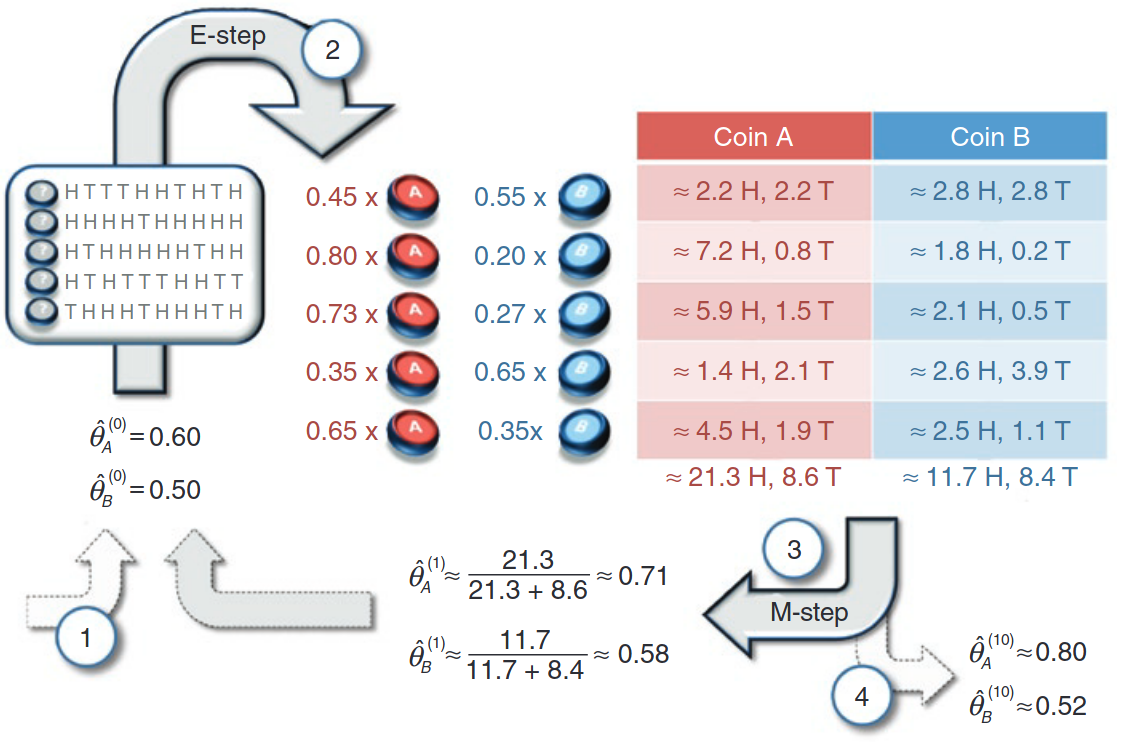
\includegraphics[width=0.7\textwidth]{chapters/BayesianNetworksLearning/mixture}
  \caption{EM algorithm step in Mixture \cite{do2008expectation}}
  \label{fig:mixture}
\end{figure}

We are know using the figure \ref{fig:mixture} to set the example in a numerical context. We are following the numbers in the diagram.
\begin{enumerate}
  \item We are considering a prior \(\bm{\theta} = (0.6, 0.5)\), a set of \(N = 5\) samples and \(M = 10\) flips per sample.
  \item This corresponds to the \textbf{E-step}, we calculate each \(Q(z_{n}\mid x_{n}, \bm{\theta})\).
    \[
    \begin{aligned}
      Q(z_{1} = A) &= \frac{0.6^{5} 0.4^{5}}{0.6^{5}0.4^{5} + 0.5^{5}0.5^{5}} \approx 0.45 \implies Q(z_{1} = B) \approx 0.55\\
      &\mathrel{\makebox[\widthof{=}]{\vdots}} \\
      Q(z_{5} = A) &\approx 0.65 \implies Q(z_{5}=B) \approx 0.35
    \end{aligned}
    \]
  \item The \textbf{M-step} corresponds to setting
    \[
    \begin{aligned}
      \theta_{A} &= \sum_{n=1}^{5}Q(z_{n})\frac{x_{n}}{10} \approx \frac{21.3}{21.3 + 8.6} \approx 0.71\\
      \theta_{B} &\approx 0.58
    \end{aligned}
    \]
  \item Step 4 represents a possible solution after \(10\) iterations.
\end{enumerate}


\section{EM Extensions}
\subsection{Partial steps}

Making a partial M-step consist on not using the optimal parameter for the energy term, but using one with just higher energy. Finding this values can be easier than finding the optimal one and convergence still follows as the only requirement to make the likelihood increase was to increase the lower bound.

On the other hand, when studying the increase on the likelihood, we supposed that the optimal E-step was being used. In general, we cannot guarantee that a partial step would increase the likelihood, even though it is guaranteed to increase the lower bound.

Another important factor is, that the EM algorithm assumes that the energy term is possible to calculate, which may not be. As an approach to solve this situation, we can set a class of distributions \(\mathcal{Q}\), and minimize the KullBack-Leibler divergence between \(P(h \mid v, \theta)\) and a distribution \(Q \in \mathcal{Q}\), so we pick a distribution such that
\[
  Q = \argmin_{Q \in \mathcal{Q}} \KL{Q(h \mid v)}{P(h\mid v, \theta)}
\]

An extreme case is to choose \(\mathcal{Q}\) as delta functions, where the energy term is now a constant. And the optimal chose setting is
\[
Q(h^{n} \mid v^{n}) = \delta (h^{n}, h^{n}_{opt}) \hspace{2cm} h^{n}_{opt} = \argmax_{h}P(h , v^{n} \mid \theta)
\]
This is called \emph{Viterbi training} and does not guarantee that the log likelihood is being increased in each iteration.


\section{Variational Bayes}


Another method to deal with hidden variables is using \emph{Variational Bayes (VB)}, in contrast with the EM algorithm, this one uses a distribution that better represents the posterior than the one using a Maximum Likelihood approach.

Consider a simple datapoint \(x = (v,h)\), in this situation we focus our interest on the posterior distribution.
\[
  P(\theta \mid v) = \frac{P(v \mid \theta)P(\theta)}{P(v)} = \frac{1}{P(v)}\int_{h}P(v,h \mid \theta)P(\theta)
\]

Variational Bayes assumes the joint hidden and parameter posterior can be approximated as the product of two distributions, one over the hidden variable and one over the parameter such that
\[
  P(h ,\theta \mid v) \approx Q(h)Q(\theta)\footnote{We use the same letter for both distributions, as they can be differenced from the context.}
\]

\begin{remark}
  By doing this assumption, we are also assuming that the posterior can be approximated with \(Q(\theta)\)
  \[
    P(\theta \mid v) = \int_{h} P(\theta, h \mid v) \approx \int_{h} Q(h)Q(\theta) = Q(\theta)
  \]
  For this reason, the main goal of the algorithm is to make this approximation as tightest as possible with an iterative method that calculates both \(Q(\theta)\) and \(Q(h)\) distributions.
\end{remark}

To achieve that, we minimize the Kullback-Leibler divergence between them.
\[
  \KL{Q(h)Q(\theta)}{P(h, \theta \mid v)} = \E{Q(h)}{\log{Q(h)}} + \E{Q(\theta)}{\log{Q(\theta)}} - \E{Q(h)Q(\theta)}{\log{P(h,\theta \mid v)}} \geq 0
\]

We use that \(\log{P(v)}\) is independent from \(Q(h)Q(\theta)\) to get the desired inequality.
\[
  \begin{aligned}
    0 &\leq \E{Q(h)}{\log{Q(h)}} + \E{Q(\theta)}{\log{Q(\theta)}} - \E{Q(h)Q(\theta)}{\log{P(h,\theta \mid v)}}\\
    &= \E{Q(h)}{\log{Q(h)}} + \E{Q(\theta)}{\log{Q(\theta)}} - \E{Q(h)Q(\theta)}{\log{\frac{P(h,\theta,v)}{P(v)}}} \\
    &=\E{Q(h)}{\log{Q(h)}} + \E{Q(\theta)}{\log{Q(\theta)}} - \E{Q(h)Q(\theta)}{\log{P(h,\theta, v)}} + \E{Q(h)Q(\theta)}{\log{P(v)}} \\
    &= \E{Q(h)}{\log{Q(h)}} + \E{Q(\theta)}{\log{Q(\theta)}} - \E{Q(h)Q(\theta)}{\log{P(h,\theta, v)}} + \log{P(v)} \\
  \end{aligned}
\]
We got the following lower bound
\[
  \log{P(v)} \geq -\E{Q(h)}{\log{Q(h)}}- \E{Q(\theta)}{\log{Q(\theta)}} + \E{Q(h)Q(\theta)}{\log{P(h,\theta, v)}}
\]
So that minimizing the Kullback-Leibler divergence is equivalent to find the tightest lower bound.

The procedure is then split in two steps to keep the structure of the EM algorithm.

\begin{itemize}
  \item \textbf{E-step}. Given a fixed \(Q(\theta)\), minimize the Kullback-Leibler divergence.
    \[
    Q^{new}(h) = \argmin_{Q(h)}\KL{Q(h)Q(\theta)}{P(h,\theta \mid v)}
    \]

  \item \textbf{M-step}. Given a fixed \(Q(h)\), minimize the Kullback-Leibler divergence.
    \[
    Q^{new}(\theta) = \argmin_{Q(\theta)}\KL{Q(h)Q(\theta)}{P(h,\theta \mid v)}
    \]
\end{itemize}

As in the case of the EM algorithm, each iterations guarantees an increase in the lower bound of the marginal likelihood, but increasing the marginal likelihood itself is not guaranteed.

When using an i.i.d dataset \((\V, \mathcal{H})\), we may assume that \(Q(\mathcal{H})\) can be factorized:
\[
  Q(h_{1}, \dots, h_{N}) = \prod_{n=1}^{N}Q(h_{n})
\]

The lower bound to the marginal likelihood is then written as a summation of the bounds on each datapoint.
\[
  \log{P(\V)} \geq \mathlarger{\sum_{n}} -\E{Q(h_{n})}{\log{Q(h_{n})}}- \E{Q(\theta)}{\log{Q(\theta)}} + \E{Q(h_{n})Q(\theta)}{\log{P(v_{n}, h_{n},\theta)}}
\]

\subsection{VB is a generalization of the EM algorithm}

We start considering a distribution over the parameter that summarizes the information in the optimal point, let \(\theta_{opt}\) be the optimal value of \(\theta\).
\[
  Q(\theta) = \delta(\theta - \theta_{opt})
\]
The lower bound takes the form
\[
  \log{P(v)} \geq - \E{Q(h)}{\log{Q(h)}} + \E{Q(h)}{\log{P(h, v, \theta_{opt})}} + \text{ const. }
\]
The M-step is then picking the optimal parameter \(\theta_{opt}\) given a fixed \(Q(h)\):
\[
  \begin{aligned}
    \theta_{opt} &= \argmax_{\theta} \Big( \E{Q(h)}{\log{P(v,h,\theta)}} \Big)\\
    &=  \argmax_{\theta} \Big( \E{Q(h)}{\log{P(v, h \mid \theta)P(\theta)}} \Big) \\
    &= \argmax_{\theta} \Big( \E{Q(h)}{\log{P(v,h \mid\theta)}} + \log{P(\theta)} \Big) \\
  \end{aligned}
\]

If we take a flat prior (\(P(\theta) \)  constant), this term is equivalent to the energy one in the EM bound \(\E{Q(h\mid v)}{\log{P(h,v \mid \theta)}}\).

The VB E-step consists on minimizing \(\KL{Q(h)}{P(h,\theta_{opt} \mid v)}\) over \(Q(h)\), as
\[
  \begin{aligned}
    \KL{Q(h)}{P(h\mid \theta_{opt}, v)} &= \E{Q(h)}{Q(h)} - \E{Q(h)}{P(h \mid \theta_{opt}, v)} \\
    &= \E{Q(h)}{Q(h)} - \E{Q(h)}{\frac{P(h, \theta_{opt} \mid v)}{P(\theta_{opt})}}  \\
    &= \E{Q(h)}{Q(h)} - \frac{1}{P(\theta_{opt})}\E{Q(h)}{P(h, \theta_{opt} \mid v)}
\end{aligned}
\]
where \(P(\theta_{opt})\) is a constant and
\[
\KL{Q(h)}{P(h, \theta_{opt} \mid v)} = \E{Q(h)}{Q(h)} - \E{Q(h)}{P(h, \theta_{opt} \mid v)}
\]
Then, as  he E-step of the EM algorithm consisted on minimizing the Kullback-Leibler divergence \(\KL{Q(h \mid v)}{P(h \mid v, \theta)}\), both steps are equivalent.

\begin{remark}
  Expectation Maximization algorithm is a special case of Variational Bayes with a flat prior and a delta function as the parameter posterior approximation.
\end{remark}


\ctparttext{
  \color{black}
  \begin{center}

  \end{center}
}
\part{Practical case with InferPy}

\chapter{InferPy usage}

InferPy is a high-level API for probabilistic modeling written in Python and capable of running on top of Edward and Tensorflow. InferPy's API is strongly inspired by Keras and it has a focus on enabling flexible data processing, easy-to-code probablistic modeling, scalable inference and robust model validation.


\chapter{Gaussian Mixture}

\clearpage
\nocite{*}
\bibliographystyle{authordate1}
\bibliography{refs}
\end{document}
